\documentclass[letterpaper,twocolumn,10pt]{article}
%DIF LATEXDIFF DIFFERENCE FILE
%DIF DEL ../nsdi16/mb.tex   Fri Feb 12 22:51:22 2016
%DIF ADD mb.tex             Fri Feb 12 23:02:06 2016

\usepackage[subtle]{savetrees-clean}
\usepackage{usenix}
\usepackage{times}
\usepackage{amsmath}
\usepackage{multirow}
% SOME OF OUR DEFINITIONS
\usepackage[keeplastbox]{flushend}


\usepackage{xspace}
%DIF 13c13
%DIF < \newcommand{\sys}{MBArk\xspace}
%DIF -------
\newcommand{\sys}{Embark\xspace} %DIF > 
%DIF -------
\newcommand{\RM}{RM\xspace}

% MBArk
% EMBArk

\usepackage[compact]{titlesec}
\titlespacing*{\section}{0pt}{4pt}{0pt}
\titlespacing*{\subsection}{0pt}{4pt}{0pt}
\titlespacing*{\subsubsection}{0pt}{4pt}{0pt}
\usepackage[small]{caption}
\usepackage{fancyvrb}
\usepackage{listings}
\usepackage[T1]{fontenc}

%DIF 28-29d28
%DIF < 
%DIF < 
%DIF -------
% more compact than computer modern
\usepackage{times}

% Typewriter Font: Latin Modern Typewriter Proportional
\renewcommand*{\ttdefault}{lmvtt}

\lstset{
  basicstyle=\footnotesize\ttfamily, 
    columns=fullflexible,
    keepspaces=true,
}

\usepackage{subfigure}
\usepackage{ifpdf}
\usepackage[usenames,dvipsnames]{color}
\usepackage[hyphens]{url}
\usepackage[breaklinks, pdfborder={0 0 0}]{hyperref}
\hypersetup{
  backref=true
    bookmarksnumbered,
    colorlinks=true,
    pdfstartview={FitH},
    citecolor={blue},
    linkcolor={blue},
    urlcolor={blue},
    citecolor={blue},
    pdfpagemode={UseOutlines}
}

\usepackage[noend]{algpseudocode}

% edit the comments 
\usepackage{eqparbox}
\renewcommand{\algorithmiccomment}[1]{\eqparbox{COMMENT}{// {\emph #1}}}

\usepackage{enumitem}

\newcommand{\tbd}[1]{}
\newcommand{\ie}{{\it i.e.}}
\newcommand{\eg}{{\it e.g.}}
\newcommand{\etc}{{\it etc.}}


\newcommand{\mypara}[1]{\medskip\noindent{\bf {#1}.}~}
\newcommand{\bpara}[1]{\noindent{\bf {#1}.}~}
\newcommand{\submypara}[1]{\medskip\noindent{\it {#1}.}~}
\newcommand{\chk}{$\checkmark$}
\newcommand{\dsh}{{\bf --}}
\newcommand{\til}{{\bf\large \textasciitilde}}
\usepackage{rotating}

\usepackage{framed}
\FrameSep4pt
\setlength{\topsep}{0pt}

\newcommand{\CTE}{CTE\xspace}
\newcommand{\Name}{APLOMB\xspace}
\newcommand{\Nameplus}{{APLOMB+}\xspace}
\newcommand{\NameArch}{{\sc APLOMB}\xspace}

%DIF 90a88-104
% ENCRYPTION NOTATION %DIF > 
 %DIF > 
\newcommand{\ov}[1]{\overline{#1}} %DIF > 
 %DIF > 
\newcommand{\pmatch}{PrefixMatch} %DIF > 
 %DIF > 
\newcommand{\plen}{\mathsf{prefix\_len}} %DIF > 
\newcommand{\slen}{\mathsf{suffix\_len}} %DIF > 
\newcommand{\ptlen}{\mathsf{pt\_len}} %DIF > 
 %DIF > 
 %DIF > 
 %DIF > 
\newcommand{\comment}[1]{\hfill {\footnotesize // #1}} %DIF > 
 %DIF > 
\newcommand{\prefixes}{\mathsf{prefixes}} %DIF > 
\newcommand{\seed}{\mathsf{seed}} %DIF > 
 %DIF > 
%DIF -------
% RESULTS

\newcommand{\generalFHEslowdown}{9\xspace}
\newcommand{\squaregeneralFHEslowdown}{18}
\newcommand{\strawmanslowdown}{10^6}
\newcommand{\setuptime}{414 s}
\newcommand{\strawmansetuptimesslower}{1.8 \cdot 10^3}

\usepackage{enumitem}
\setlist[itemize]{itemsep=0.00cm}
\setlist[itemize]{parsep=0.01cm}
%\setlist[itemize]{parskip=0.01cm}

\newenvironment{myitemize}
{ \begin{itemize}[nolistsep,leftmargin=0.15in]
  \setlength{\itemsep}{0.5pt}
  \setlength{\parskip}{0.9pt}
  \setlength{\parsep}{0.1pt}     }
{ \end{itemize}                  } 

\newcommand{\simplequote}[1]{\\\noindent{\it``{#1}''}\linebreak[3]}
\newcommand{\green}[1]{{\color{ForestGreen}{#1}}}


% our encryption scheme
\newcommand{\bbenc}{DPIEnc\xspace}
\newcommand{\bbdetect}{\sys Detect\xspace}

\newcommand{\RG}{RG\xspace}
\newcommand{\MB}{MB\xspace}

\newcommand{\sslk}{k_{\mathsf{SSL}}}
\newcommand{\bbG}{\mathbb{G}}

\newcommand{\garble}{\mathsf{Garble}}
\newcommand{\eval}{\mathsf{Eval}}
\newcommand{\keygen}{\mathsf{KeyGen}}
\newcommand{\Enc}{\mathsf{Enc}}
\newcommand{\kwenc}{\mathsf{KWEnc}}
\newcommand{\enc}{\Enc}
\newcommand{\en}{\mathsf{enc}}
\newcommand{\encleft}{\mathsf{EncLeft}}
\newcommand{\encright}{\mathsf{EncRight}}
\newcommand{\match}{\mathsf{Match}}

\newcommand{\sig}{\mathsf{sig}}
\newcommand{\ct}{\mathsf{ct}}
\newcommand{\sno}{\mathsf{serial\_no}}
\newcommand{\dirtyrange}{\mathsf{dirtyrange}}

\renewcommand{\mod}{\mathsf{mod}\xspace}

\newcommand{\low}{\mathsf{low}\xspace}
\newcommand{\high}{\mathsf{high}\xspace}
\newcommand{\prf}{\mathsf{prf}\xspace}
%DIF 145a160
\newcommand{\prefix}{\mathsf{prefix}\xspace} %DIF > 
%DIF -------
\newcommand{\IV}{\mathsf{IV}}

\newcommand{\twosnortcom}{67\%}
\newcommand{\twosnortemerge}{42\%}


\newcommand{\SSL}{\mathsf{SSL}}
\newcommand{\rand}{\mathsf{rand}}
\newcommand{\salt}{\mathsf{salt}}

\newcommand{\mf}[1]{ {\fontfamily{cmtt}\selectfont#1}}

\newcommand{\ALGORITHM}[4]{%  name, llabel, intro, \items    
  \let\oldi\labelenumi
    \let\oldii\labelenumii
    \let\oldiii\labelenumiii
    \renewcommand{\labelenumi}{\arabic{enumi}: }
  \renewcommand{\labelenumii}{\arabic{enumi}.\arabic{enumii}: }
  \renewcommand{\labelenumiii}{\arabic{enumi}.\arabic{enumii}.\arabic{enumiii}: }                                     
%DIF 164-165c180-181
%DIF <   \noindent \textbf{#1:} \label{#2} 
%DIF < #3
%DIF -------
  \noindent \textbf{#1} \label{#2} %DIF > 
(#3): %DIF > 
%DIF -------
  \vspace{0.13\baselineskip}
  \begin{enumerate}[noitemsep,nolistsep]\itemsep=0.1\baselineskip
#4
    \end{enumerate}
  \let\labelenumi\oldi
    \let\labelenumii\oldii
    \let\labelenumiii\oldii  
}

%\newcommand{\subparagraph}{\paragraph}
%\usepackage[compact]{titlesec}

\newcommand{\tickYes}{\checkmark}
%DIF 179c195
%DIF < \newcommand{\raluca}[1]{}
%DIF -------
\newcommand{\raluca}[1]{{\color{Red}{\bf TODO: }}} %DIF > 
%DIF -------
\newcommand{\sr}[1]{{\color{CarnationPink} SR: {#1}}} % :)
\newcommand{\clan}[1]{{\color{SkyBlue} CL: {#1}}} % :)
\newcommand{\qu}[1]{{\color{Magenta}  {\bf Question:} {#1}}} 
\newcommand{\warning}[1]{{\color{Red}{\bf Warning: #1}}}
%DIF 184-185c200-201
%DIF < %\newcommand{\todo}[1]{{\color{Red}{\bf TODO: #1}}}
%DIF < \newcommand{\todo}[1]{}
%DIF -------
\newcommand{\todo}[1]{{\color{Red}{\bf }}} %DIF > 
%\newcommand{\todo}[1]{} %DIF > 
%DIF -------
\newcommand{\justine}[1]{{\color{Green}{\bf JS: #1}}}

\newcommand{\aes}{\mathsf{AES}}
\newcommand{\encr}{\mathsf{enc\_r}}


% Compact itemize and enumerate.  Note that they use the same counters and                         
% symbols as the usual itemize and enumerate environments.                                         
\makeatletter
\def\compactify{\itemsep=3pt plus3pt \topsep=3pt plus3pt \partopsep=0pt
  \parsep=0pt \leftmargin=1.3em}
  \let\latexusecounter=\usecounter
  \def\CompactItemize{%                                                                              
    \ifnum \@itemdepth >\thr@@\@toodeep\else
      \advance\@itemdepth\@ne
      \edef\@itemitem{labelitem\romannumeral\the\@itemdepth}%                                        
      \expandafter
      \list
      \csname\@itemitem\endcsname
      {\compactify\def\makelabel##1{\hss\llap{##1}}}%                                              
    \fi}
    \let\endCompactItemize\endlist
    \newenvironment{CompactEnumerate}
{\def\usecounter{\compactify\latexusecounter}
  \begin{enumerate}}
{\end{enumerate}\let\usecounter=\latexusecounter}
\makeatother


% Tweaks
\setlength{\abovecaptionskip}{2pt}
\setlength{\belowcaptionskip}{-15pt}
\frenchspacing
\makeatletter
\g@addto@macro\normalsize{%
  \setlength\abovedisplayskip{2pt}
  \setlength\belowdisplayskip{2pt}
  \setlength\abovedisplayshortskip{2pt}
  \setlength\belowdisplayshortskip{2pt}
}
\makeatother

% Title, authors
\date{}

\title{
  %American capitalization structure.
  \sys: Securely Outsourcing Middleboxes to the Cloud
}

\newcommand{\superscript}[1]{\ensuremath{^{\textrm{#1}}}}
\newcommand{\affila}{\superscript{*}}
\newcommand{\affilb}{\superscript{\dag}}
\newcommand{\affilc}{\superscript{\ddag}}

\author{
  {\rm Chang Lan} \qquad 
  {\rm Justine Sherry} \qquad 
  {\rm Raluca Ada Popa} \qquad 
  {\rm Sylvia Ratnasamy} \qquad 
  {\rm Zhi Liu\affila} \\
  UC Berkeley \qquad \affila Tsinghua University
}
%DIF PREAMBLE EXTENSION ADDED BY LATEXDIFF
%DIF UNDERLINE PREAMBLE %DIF PREAMBLE
\RequirePackage[normalem]{ulem} %DIF PREAMBLE
\RequirePackage{color}\definecolor{RED}{rgb}{1,0,0}\definecolor{BLUE}{rgb}{0,0,1} %DIF PREAMBLE
\providecommand{\DIFaddtex}[1]{{\protect\color{blue}\uwave{#1}}} %DIF PREAMBLE
\providecommand{\DIFdeltex}[1]{{\protect\color{red}\sout{#1}}}                      %DIF PREAMBLE
%DIF SAFE PREAMBLE %DIF PREAMBLE
\providecommand{\DIFaddbegin}{} %DIF PREAMBLE
\providecommand{\DIFaddend}{} %DIF PREAMBLE
\providecommand{\DIFdelbegin}{} %DIF PREAMBLE
\providecommand{\DIFdelend}{} %DIF PREAMBLE
%DIF FLOATSAFE PREAMBLE %DIF PREAMBLE
\providecommand{\DIFaddFL}[1]{\DIFadd{#1}} %DIF PREAMBLE
\providecommand{\DIFdelFL}[1]{\DIFdel{#1}} %DIF PREAMBLE
\providecommand{\DIFaddbeginFL}{} %DIF PREAMBLE
\providecommand{\DIFaddendFL}{} %DIF PREAMBLE
\providecommand{\DIFdelbeginFL}{} %DIF PREAMBLE
\providecommand{\DIFdelendFL}{} %DIF PREAMBLE
%DIF END PREAMBLE EXTENSION ADDED BY LATEXDIFF
%DIF PREAMBLE EXTENSION ADDED BY LATEXDIFF
%DIF HYPERREF PREAMBLE %DIF PREAMBLE
\providecommand{\DIFadd}[1]{\texorpdfstring{\DIFaddtex{#1}}{#1}} %DIF PREAMBLE
\providecommand{\DIFdel}[1]{\texorpdfstring{\DIFdeltex{#1}}{}} %DIF PREAMBLE
%DIF END PREAMBLE EXTENSION ADDED BY LATEXDIFF

\begin{document}

\maketitle

%!TEX root = mb.tex

\begin{abstract}
\todo{if we are under space limit, you can move this down a bit as it is quite squeezed}
{\it %%Sylvia and scott style is to put the abstract in italics.
It is increasingly common for enterprises and other organizations to outsource network processing -- such as firewalling and caching -- to the cloud, just as they often outsource compute and storage.
However, this poses a threat to enterprise confidentiality because the cloud provider gains access to the organization's traffic.

We design and build \sys, the first system that enables a cloud provider to support middlebox outsourcing while maintaining the client's confidentiality. \sys encrypts the traffic that reaches the cloud and enables the cloud to process the  encrypted traffic {without decrypting it}.
\sys supports a wide-range of middleboxes such as firewalls, NATs, web proxies, load balancers,  \DIFdelbegin \DIFdel{intrusion prevention systems, }\DIFdelend and data exfiltration systems. Our evaluation shows that \sys supports these applications with competitive performance: per-middlebox throughput is affected by at worst 2.7\%.
}
\end{abstract}


%!TEX root = mb.tex 

\section{Introduction}\label{sec:intro}


%DIF > \begin{table*}[t]
%DIF > \centering
%DIF > \small
%DIF > \hspace{-2pt}
%DIF > \begin{tabular}{l|l|l}
%DIF > \hline
%DIF > {\bf Middlebox} & {\bf Requirements} & {\bf Scheme} \\ \hline
%DIF > IP Firewall & 
%DIF > \parbox {10cm}{
%DIF > \begin{flalign*}
%DIF > (SIP,\ DIP,\ SP,\ DP,\ P)\ \rightarrow\ action\ a \quad \Rightarrow \quad (SIP',\ DIP',\ SP',\ DP',\ P')\ \rightarrow\ action\ a &
%DIF > \end{flalign*}
%DIF > } & PrefixMatch \\ \hline
%DIF > 
%DIF > NAT (NAPT) & 
%DIF > \parbox {10cm}{
%DIF > \begin{flalign*}
%DIF > \text{Injective: } & (SIP_1, SP_1)\ \neq\ (SIP_2, SP_2) \quad \Rightarrow \quad (SIP_1', SP_1')\ \neq\ (SIP_2', SP_2') \\
%DIF > \text{Deterministic: } & (SIP_1, SP_1)\ =\ (SIP_2, SP_2) \quad \Rightarrow \quad (SIP_1', SP_1')\ =\ (SIP_2', SP_2')
%DIF > \end{flalign*}
%DIF > } 
%DIF > & PrefixMatch \\ \hline
%DIF > 
%DIF > L3 Load Balancer (ECMP) &
%DIF > \parbox {10cm}{
%DIF > \begin{flalign*}
%DIF > \text{Deterministic: } & (SIP_1, DIP_1, SP_1, DP_1, P_1)\ =\ (SIP_2, DIP_2, SP_2, DP_2, P_2) \quad \Rightarrow \\
%DIF > & (SIP_1', DIP_1', SP_1', DP_1', P_1')\ =\ (SIP_2', DIP_2', SP_2', DP_2', P_2') 
%DIF > \end{flalign*}
%DIF > }
%DIF > & PrefixMatch \\ \hline
%DIF > 
%DIF > L4 Load Balancer &
%DIF > \parbox {10cm}{
%DIF > \begin{flalign*}
%DIF >     \text{Injective: } & (SIP_1, DIP_1, SP_1, DP_1, P_1)\ \neq\ (SIP_2, DIP_2, SP_2, DP_2, P_2) \quad \Rightarrow \\
%DIF >     & (SIP_1', DIP_1', SP_1', DP_1', P_1')\ \neq\ (SIP_2', DIP_2', SP_2', DP_2', P_2') \\
%DIF >     \text{Deterministic: } & (SIP_1, DIP_1, SP_1, DP_1, P_1)\ =\ (SIP_2, DIP_2, SP_2, DP_2, P_2) \quad \Rightarrow \\ 
%DIF >     & (SIP_1', DIP_1', SP_1', DP_1', P_1')\ =\ (SIP_2', DIP_2', SP_2', DP_2', P_2')
%DIF > \end{flalign*}
%DIF > }
%DIF > & PrefixMatch \\ \hline
%DIF > 
%DIF > Deep Packet Inspection &
%DIF > \parbox {10cm}{
%DIF > \begin{flalign*}
%DIF > & keyword \in stream \quad \Rightarrow \quad keyword' \in stream'
%DIF > \end{flalign*}
%DIF > } &
%DIF > KeywordMatch \\ \hline
%DIF > 
%DIF > Parental Filter &
%DIF > \parbox {10cm}{
%DIF > \begin{flalign*}
%DIF > & URL \in HTTP\ Header \quad \Rightarrow \quad URL' \in HTTP\ Header'
%DIF > \end{flalign*}
%DIF > } &
%DIF > KeywordMatch \\ \hline
%DIF > 
%DIF > HTTP Proxy / Cache &
%DIF > \parbox {10cm}{
%DIF > \begin{flalign*}
%DIF > & URL \in HTTP\ Header \quad \Rightarrow \quad URL' \in HTTP\ Header'
%DIF > \end{flalign*}
%DIF > } &
%DIF > KeywordMatch \\ \hline
%DIF > 
%DIF > \end{tabular}
%DIF > \caption[]{Middleboxes supported by \sys. Middleboxes are also labeled with their requirement on the encryption schemes. $(SIP, DIP, SP, DP, P)$ denotes the 5-tuple of a connection. $x'$ is the encryption of $x$.\label{tbl:mbreqs}} 
%DIF > \end{table*}
%DIF > 
\DIFaddbegin 


%DIF > %%%%%%%%%%%%%%%%%%%





\todo{fix the text below in comments}

%DIF > A useful piece of text:
%DIF > 
%DIF > Table 1 presents the ``textbook'' functionality of each middlebox supported. This functionality is the basica functionality
%DIF > of this box as presented in textbook .. and RFC ...
%DIF > Note that some of these middleboxes have become even more complex, supporting additional functionality not present in
%DIF > Table 1. Such functionality may or may be supported by \sys. \sys does not support all complex functionalities out there adn we discuss in \S what we do not support. Make clear that the table spells out precisely what we can support and what not. 
%DIF > 
%DIF > In Table XX, we provide the functionality that \sys provides. This covers the functionality of xxx of above and most of the one
%DIF > below. Moreover, in eval, we show that we support at least a real middlebox from each of hte examples above. 
%DIF > 
%DIF > ------




\DIFaddend Middleboxes such as firewalls, NATs, and proxies, have grown to be a vital part of modern networks, but are 
also widely recognized as bringing significant problems including high cost, inflexibility, and complex management.  
These problems have led both research and industry to explore an alternate approach: moving middlebox functionality out of dedicated boxes and into 
software applications that run multiplexed on commodity server hardware~\cite{mb-manifesto,comb,aplomb,opennf,clickos,flowtags,etsi-nfv,domain20,opnfv}.
This approach -- termed Network Function Virtualization (NFV) in industry -- promises many advantages including the cost benefits of commodity infrastructure, 
the efficiencies of statistical multiplexing, and the flexibility of software solutions. 
In a short time, NFV has gained a significant momentum with over 270 industry participants~\cite{etsi-nfv} and a number of emerging product offerings~\cite{brocade,dell,juniper}.

Leveraging the above trend, several efforts are exploring a new model for middlebox deployment in which a third-party offers middlebox processing as a  
\emph{service}.
Such a service may be hosted in a public cloud~\cite{aplomb,zscaler,aryaka} or in private clouds embedded within an ISP 
infrastructure~\cite{domain20, telefonica}.  
This service model allows customers such as enterprises to ``outsource'' middleboxes from their networks entirely, and hence promises many of the known benefits of cloud computing  such as decreased costs and ease of management.%: decreased costs, ease of management, \etc{}.

However, outsourcing middleboxes brings a new challenge: the confidentiality of the traffic. 
Today, in order to process an organization's traffic, the cloud sees the traffic {\em unencrypted}.  This means that the cloud 
now has access to potentially sensitive packet payloads and headers. This is 
worrisome considering the number of documented data breaches by cloud employees or hackers~\cite{PrivacyRecords,databreach}.
Hence, an important question is: can we enable a third party to process traffic for an enterprise, {\em without seeing the enterprise's traffic}?

To address this, we designed and implemented \sys, the first system to allow an enterprise to outsource  a comprehensive set of enterprise middleboxes  to a cloud provider, while keeping its traffic confidential. 
Middleboxes in \sys operate directly over {\it encrypted} traffic. %without decrypting the traffic. 


In recent work, we designed a system called BlindBox to operate on encrypted traffic for a {\em specific} class of middleboxes: Deep Packet Inspection~\cite{blindbox} -- middleboxes that examine only the payload of packets. 
However, BlindBox is far from sufficient for this setting because
 (1) it has restricted functionality that does not support all middleboxes required for outsourcing, and (2) it has prohibitive performance overheads.

 Regarding functionality, BlindBox enables equality-based operations on  encrypted payloads of packets, which supports certain DPI devices. However, this excludes middleboxes such as firewalls, proxies, load balancers, NAT,  and those DPI devices that also examine packet headers, because these need the ability to examine packet headers and/or perform range queries. 
 % I added this packet header thing due to NAT
 % even though some of these MB only do exact, the architecture that puts them all together is new
 Achieving such generality provided new challenges to \sys. 
As we discuss below, such middleboxes require a new encryption scheme and, moreover, a system design that supports all middleboxes {\it simultaneously}: for performance, adoption and extensibility, it does not suffice to craft {\it n} different designs to support {\it n} classes of middleboxes. 

 
Regarding performance, BlindBox has a prohibitive setup time of 97s per-connection. 
\sys's setting targets enterprise outsourcing where BlindBox targets end hosts connecting to arbitrary middleboxes. This difference brings \sys new opportunities: it
not only allows us to remove the setup overhead, but also to achieve better deployability and higher security, as we discuss in \S\ref{sec:bbarch}. 

\sys supports a \DIFdelbegin \DIFdel{comprehensive set }\DIFdelend \DIFaddbegin \DIFadd{wide range }\DIFaddend of middleboxes with practical performance. These cover all the applications that are typically outsourced as surveyed in~\cite{aplomb}. Table~\ref{tbl:mbreqs} lists these applications. 
%DIF > It also lists each middlebox's requirement on the encryption schemes. We derive those requirements based on the existing papers, documents, or implementations. 
\sys achieves this through a combination of systems and cryptographic innovations, as follows.

From a cryptographic perspective, \sys provides a new and fast encryption scheme called \DIFdelbegin \DIFdel{RangeMatch  }\DIFdelend \DIFaddbegin \DIFadd{PrefixMatch  }\DIFaddend to enable the provider to perform prefix matching (\eg{}, if an IP address is in the subdomain 56.24.67.0/16) or port range detection (\eg{}, if a port is in the range 1000-2000). %DIF < The design of RangeMatch is highly inspired from the network setting.
 \DIFdelbegin \DIFdel{Prior to RangeMatch}\DIFdelend \DIFaddbegin \DIFadd{Prior to PrefixMatch}\DIFaddend , there was no mechanism that provided the functionality, performance, and  security needed in our setting. The closest practical encryption schemes are Order-Preserving Encryption (OPE)~\cite{boldyreva:ope,popa:mope,popa:cryptdb}. 
However, these schemes are four orders of magnitude slower than {\it \DIFdelbegin \DIFdel{RangeMatch}\DIFdelend \DIFaddbegin \DIFadd{PrefixMatch}\DIFaddend } making them unusable for our network setting. At the same time, \DIFdelbegin \DIFdel{RangeMatch }\DIFdelend \DIFaddbegin \DIFadd{PrefixMatch }\DIFaddend provides stronger security guarantees than these schemes, which leak unnecessary information to the provider: for every encrypted value, {\em \DIFdelbegin \DIFdel{RangeMatch}\DIFdelend \DIFaddbegin \DIFadd{PrefixMatch}\DIFaddend } reveals only whether the value lies within a range or not, whereas OPE reveals the total ordering among all values.

  From a systems design perspective, one of the key insights behind \sys is to keep packet formats unchanged: an encrypted IP packet is structured just as a normal IP packet, with each field (e.g., source address) containing an encrypted value of that field.
  This strategy ensures that encrypted packets never appear invalid, e.g., to existing network interfaces, forwarding algorithms, and error checking. 
  We choose which encryption scheme to use for each field based on the processing operations applied by typical middleboxes; this results in an encrypted packet that simultaneously supports {\it all} of the wide range of middleboxes we outsource.

  Another systems insight is that by {\it combining} standard packet formats with \DIFdelbegin \DIFdel{RangeMatch}\DIFdelend \DIFaddbegin \DIFadd{PrefixMatch}\DIFaddend , \sys can retain compatibility with existing classification algorithms and obtain good performance for middleboxes operating over header fields.
  \DIFdelbegin \DIFdel{RangeMatch }\DIFdelend \DIFaddbegin \DIFadd{PrefixMatch }\DIFaddend ensures that comparisons (such as $\leq$) function normally, hence, a middlebox receiving an encrypted packet can simply perform the normal set of `fast-path' packet processing operations unmodified.
  Importantly, middleboxes can continue to take advantage of highly-efficient packet classification algorithms~\cite{packet_classif} as already implemented, and which are among the more expensive tasks in \DIFdelbegin \DIFdel{in }\DIFdelend software middleboxes~\cite{comb, ethan-paper}.
  Furthermore, even software-based NFV deployments make use of some hardware forwarding components, \eg{} NIC multiqueue flow hashing~\cite{nicdocument}, `whitebox' switches~\cite{whitebox}, and error detection in NICs and switches~\cite{nicdocument, ciscov6}; \sys is compatible with all of these.

 
 \DIFaddbegin \begin{table}[t]
\centering
\small
\DIFaddFL{\hspace{-2pt}
}\begin{tabular}{c|c}
\hline
{\bf \DIFaddFL{Middlebox}} &  {\bf \DIFaddFL{Scheme}} \\ \hline
\DIFaddFL{IP Firewall }& 
 \DIFaddFL{PrefixMatch }\\ 

\DIFaddFL{NAT (NAPT) }& 
 \DIFaddFL{PrefixMatch }\\

\DIFaddFL{L3 Load Balancer (ECMP) }&
 \DIFaddFL{PrefixMatch }\\ 

\DIFaddFL{L4 Load Balancer }&
 \DIFaddFL{PrefixMatch }\\ 

\DIFaddFL{Deep Packet Inspection }&

\DIFaddFL{KeywordMatch }\\ 

\DIFaddFL{Parental Filter }&

\DIFaddFL{KeywordMatch }\\ 

\DIFaddFL{HTTP Proxy / Cache }&

\DIFaddFL{KeywordMatch }\\ 

\end{tabular}
\caption[]{\DIFaddFL{Middleboxes supported by }\sys \DIFaddFL{and the encryption scheme used.}\label{tbl:mbreqs}} 
\end{table}



\DIFaddend We implemented and evaluated \sys on EC2. \sys supports all applications typically deployed by outsourcing as surveyed in~\cite{aplomb}.
Further, \sys imposes  negligible throughput overheads at the service provider: for example, a single-core firewall operating over encrypted data achieves 9.8Gbps, equal to the same firewall over unencrypted data.
Our enterprise gateway can tunnel traffic at \DIFdelbegin \DIFdel{1.5 }\DIFdelend \DIFaddbegin \DIFadd{9.6 }\DIFaddend Gbps on a single core;  a single server can easily support 10Gbps for an small-medium enterprise.

%DIF < Relative to BlindBox, \sys is more general. But even when comparing the two directly, \sys (1) has practical performance for deployment, where BlindBox does not: connection session establishment uses standard handshakes and does not have the 97s overhead that BlindBox does; (2) is more secure: \sys can support 79.8\%-88\% of IDS rules without resorting to decryption, where BlindBox can only support 40-67\%; (3) requires no changes to endhosts, where BlindBox requires a new protocol to be supported by each client.
%DIF > \eat{Relative to BlindBox, \sys is more general. But even when comparing the two directly, \sys (1) has practical performance for deployment, where BlindBox does not: connection session establishment uses standard handshakes and does not have the 97s overhead that BlindBox does; (2) is more secure: \sys can support 79.8\%-88\% of IDS rules without resorting to decryption, where BlindBox can only support 40-67\%; (3) requires no changes to endhosts, where BlindBox requires a new protocol to be supported by each client.} 



%!TEX root = mb.tex

% 2nd fig/1st fig = 1.12 ratio
\begin{figure*}[t!]
\vspace{-10pt}
\centering
\subfigure[Enterprise to external site communication]{
  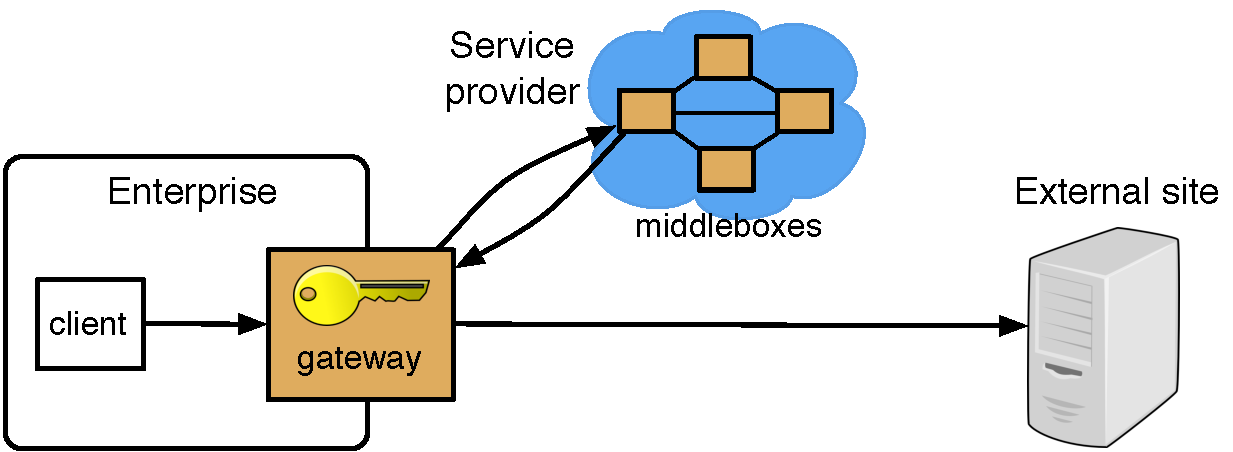
\includegraphics[width=2.8in]{fig/model_1.pdf}
  \label{fig:model1} }
%
\hfill  
\subfigure[Enterprise to enterprise communication]{
   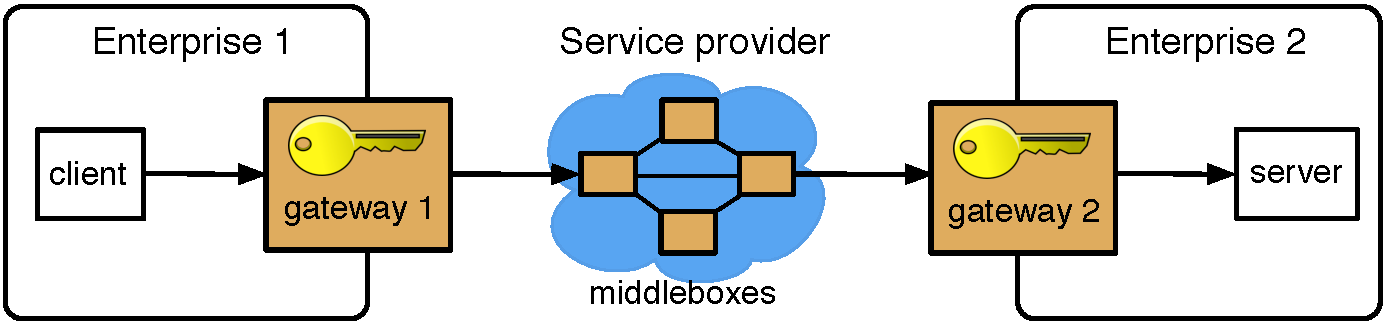
\includegraphics[width=3.2in]{fig/model_2.pdf}
     \label{fig:model2}}

     %
\caption{System architecture. APLOMB and NFV system setup with \sys encryption  at the gateway. The arrows indicate traffic from the client to the server; the response traffic follows the reverse direction. \label{fig:sys-overview}}
\end{figure*}

\section{Overview}\label{sec:overview}

In this section, we present \sys's architecture, the threat model and applications supported.


% TO CUT REMOVE: just mentino the figures and no need to explain 
\subsection{System Architecture}

\sys uses the same  architecture as APLOMB~\cite{aplomb}, a system which redirects an enterprise's traffic to the cloud for middlebox processing. \sys augments this architecture with confidentiality protection.

%The benefits of outsourcing are to delegate the burden of managing and configuring
%middleboxes (e.g., upgrading, deciding which vendor to use, monitoring), reduce costs of hardware,
%and provide elasticity and fault tolerance; hence \sys should maintain these benefits despite any changes made to to the gateway at the enterprise or middleboxes.

In the APLOMB setup, there are two parties: the enterprise(s) and the service provider (SP).
The enterprise runs a gateway (GW) which sends traffic to a set of middleboxes (MB) running in the cloud; in practice this cloud may be either a public cloud service (such as EC2), or an ISP-supported service running at a Central Office (CO).
%we already said thisThe service provider -- ISP or cloud-based -- runs a set of middleboxes. 

We illustrate the two redirection setups from APLOMB in Fig.~\ref{fig:sys-overview}.  The first setup, in Fig.~\ref{fig:model1},  occurs when the enterprise communicates with an external site: traffic goes to the cloud and back before it is sent out to the Internet. 
It is worth mentioning that APLOMB allows an optimization that saves on bandwidth and latency relative to Fig.~\ref{fig:model1}: the traffic from SP can go directly to the external site and does not have to go back through the gateway. \sys does not allow this optimization fundamentally: the traffic from SP is encrypted and cannot be understood by an external site. 
Nonetheless, as we demonstrate in \S\ref{sec:eval}, for ISP-based deployments this overhead is negligible.
For traffic within the same enterprise, where the key is known by two gateways owned by the same company, we can support the optimization as shown in Fig.~\ref{fig:model2}.

We do not delve further into the details, motivation, and gains of APLOMB's setup, and refer the reader to~\cite{aplomb} for details. 

\DIFdelbegin %DIFDELCMD < \begin{table}
%DIFDELCMD < \centering
%DIFDELCMD < \small
%DIFDELCMD < %%%
\DIFdelFL{\hspace{-2pt}
}%DIFDELCMD < \begin{tabular}{l|l|p{.45in}|p{.45in}|p{.45in}}
%DIFDELCMD < &{\bf %%%
\DIFdelFL{MB}%DIFDELCMD < }&{\bf %%%
\DIFdelFL{TCP/IP Header}%DIFDELCMD < }&{\bf %%%
\DIFdelFL{HTTP Headers}%DIFDELCMD < }&{\bf %%%
\DIFdelFL{Byte Stream}%DIFDELCMD < }\\
%DIFDELCMD < %%%
\DIFdelendFL %DIF > \eat{
%DIF > \begin{table}
%DIF > \centering
%DIF > \small
%DIF > \hspace{-2pt}
%DIF > \begin{tabular}{l|l|p{.45in}|p{.45in}|p{.45in}}
%DIF > &{\bf MB}&{\bf TCP/IP Header}&{\bf HTTP Headers}&{\bf Byte Stream}\\
%DIF > 
%DIF > \hline
%DIF > 
%DIF > \parbox[t]{1mm}{\multirow{3}{*}{\rotatebox[origin=c]{90}{Header}}}
%DIF > &IP Firewall&Range&-&-\\
%DIF > &L4 LB&Range&-&-\\
%DIF > &NAT&Exact&-&-\\
%DIF > \hline
%DIF > 
%DIF > 
%DIF > \parbox[t]{1mm}{\multirow{2}{*}{\rotatebox[origin=c]{90}{DPI}}}
%DIF > &IPS&Range&Exact&Exact\\
%DIF > &Exfiltration&Range&Exact&Exact\\
%DIF > \hline
%DIF > 
%DIF > \parbox[t]{1mm}{\multirow{3}{*}{\rotatebox[origin=c]{90}{HTTP}}}
%DIF > &Proxy&Exact&Exact&-\\
%DIF > &Parent Filter&-&Exact&-\\
%DIF > &L7 LB&Exact&Exact&-\\
%DIF > \hline
%DIF > *&VPN&-&-&-\\
%DIF > 
%DIF > \end{tabular}
%DIF > \caption[]{Middleboxes supported by \sys and categorized as Header, DPI, or HTTP middleboxes depending on what fields they access. Middleboxes are also labeled whether they perform `exact match' comparisons against rules, or `range match' comparisons against rules.\label{tbl:mbreqs}} 
%DIF > \end{table}
%DIF > }

\DIFdelbeginFL %DIFDELCMD < \hline
%DIFDELCMD < 

%DIFDELCMD < %%%
\parbox[t]{1mm}{%DIFDELCMD < \multirow{3}{*}{\rotatebox[origin=c]{90}{Header}}%%%
}
%DIFAUXCMD
%DIFDELCMD < &%%%
\DIFdelFL{IP Firewall}%DIFDELCMD < &%%%
\DIFdelFL{Range}%DIFDELCMD < &%%%
\DIFdelFL{-}%DIFDELCMD < &%%%
\DIFdelFL{-}%DIFDELCMD < \\
%DIFDELCMD < &%%%
\DIFdelFL{L4 LB}%DIFDELCMD < &%%%
\DIFdelFL{Range}%DIFDELCMD < &%%%
\DIFdelFL{-}%DIFDELCMD < &%%%
\DIFdelFL{-}%DIFDELCMD < \\
%DIFDELCMD < &%%%
\DIFdelFL{NAT}%DIFDELCMD < &%%%
\DIFdelFL{Exact}%DIFDELCMD < &%%%
\DIFdelFL{-}%DIFDELCMD < &%%%
\DIFdelFL{-}%DIFDELCMD < \\
%DIFDELCMD < \hline
%DIFDELCMD < 

%DIFDELCMD < %%%
\parbox[t]{1mm}{%DIFDELCMD < \multirow{2}{*}{\rotatebox[origin=c]{90}{DPI}}%%%
}
%DIFAUXCMD
%DIFDELCMD < &%%%
\DIFdelFL{IPS}%DIFDELCMD < &%%%
\DIFdelFL{Range}%DIFDELCMD < &%%%
\DIFdelFL{Exact}%DIFDELCMD < &%%%
\DIFdelFL{Exact}%DIFDELCMD < \\
%DIFDELCMD < &%%%
\DIFdelFL{Exfiltration}%DIFDELCMD < &%%%
\DIFdelFL{Range}%DIFDELCMD < &%%%
\DIFdelFL{Exact}%DIFDELCMD < &%%%
\DIFdelFL{Exact}%DIFDELCMD < \\
%DIFDELCMD < \hline
%DIFDELCMD < 

%DIFDELCMD < %%%
\parbox[t]{1mm}{%DIFDELCMD < \multirow{3}{*}{\rotatebox[origin=c]{90}{HTTP}}%%%
}
%DIFAUXCMD
%DIFDELCMD < &%%%
\DIFdelFL{Proxy}%DIFDELCMD < &%%%
\DIFdelFL{Exact}%DIFDELCMD < &%%%
\DIFdelFL{Exact}%DIFDELCMD < &%%%
\DIFdelFL{-}%DIFDELCMD < \\
%DIFDELCMD < &%%%
\DIFdelFL{Parent Filter}%DIFDELCMD < &%%%
\DIFdelFL{-}%DIFDELCMD < &%%%
\DIFdelFL{Exact}%DIFDELCMD < &%%%
\DIFdelFL{-}%DIFDELCMD < \\
%DIFDELCMD < &%%%
\DIFdelFL{L7 LB}%DIFDELCMD < &%%%
\DIFdelFL{Exact}%DIFDELCMD < &%%%
\DIFdelFL{Exact}%DIFDELCMD < &%%%
\DIFdelFL{-}%DIFDELCMD < \\
%DIFDELCMD < \hline
%DIFDELCMD < %%%
\DIFdelFL{*}%DIFDELCMD < &%%%
\DIFdelFL{VPN}%DIFDELCMD < &%%%
\DIFdelFL{-}%DIFDELCMD < &%%%
\DIFdelFL{-}%DIFDELCMD < &%%%
\DIFdelFL{-}%DIFDELCMD < \\
%DIFDELCMD < 

%DIFDELCMD < \end{tabular}
%DIFDELCMD < %%%
%DIFDELCMD < \caption[]{%
{%DIFAUXCMD
\DIFdelFL{Middleboxes supported by }%DIFDELCMD < \sys %%%
\DIFdelFL{and categorized as Header, DPI, or HTTP middleboxes depending on what fields they access. Middleboxes are also labeled whether they perform `exact match' comparisons against rules, or `range match' comparisons against rules.}%DIFDELCMD < \label{tbl:mbreqs}%%%
} 
%DIFAUXCMD
%DIFDELCMD < 

%DIFDELCMD < \end{table}
%DIFDELCMD < 

%DIFDELCMD < %%%
\DIFdelend \subsection{Threat Model}
%%%I know this may read superfluous to a security reader but two of the SOSP reviewers asked for this specifically -- why is a passive attacker a reasonable choice? We need this background here.
%Before defining our threat model precisely, we first provide context and background on the concerns clients have about cloud providers today.
  Clients adopt cloud services for decreased cost and ease of management. Providers are known and trusted to provide good service. 
  However, while clients trust cloud providers to perform their services correctly, there is an increasing concern that cloud providers may access or leak confidential data in the process of providing service.
  Reports in the popular press describe companies selling customer data to marketers~\cite{radioshack}, disgruntled employees snooping or exporting data~\cite{att}, and hackers gaining access to data on clouds~\cite{databreach,PrivacyRecords}.
  This type of threat is referred to as an `honest but curious' or `passive'~\cite{goodrich} attacker: a party who is trusted to handle the data and deliver service correctly, but who looks at the data, and steals or exports it.  Hence, \sys aims to stop these attackers.
  Such an attacker differs from the `active' attacker, who manipulates data or deviates from the protocol it is supposed to run~\cite{goodrich}.
%
Hence, we consider that such a passive attacker has gained access 
to {\em all the data at SP}.
This includes any traffic and communication SP receives from the 
gateway, any logged information, cloud state, and so on.  

We assume that the gateways are managed by the enterprise and hence trusted; they do not leak information.
%The goal of \sys is to protect the privacy of the traffic against an attacker at the service provider  
%cloud employee, or hacker gaining access to cloud machines). 

%The existence of this gateway is they key difference between BlindBox and \sys and not only changes our trust model, but also allows us to improve performance, privacy, and deployability relative to BlindBox, as we will discuss lated in this paper.

Some middleboxes (such as intrusion or exfiltration detection) have a threat model
of their own about the two endpoints communicating. For example, intrusion detection assumes that 
one of the endpoints could misbehave, but at most one of them misbehaves~\cite{Bro}.  
%(indeed, if both misbehave, they can send attack traffic to each other encrypted with a shared symmetric key and fundamentally
%no one can detect such an attack).  
We preserve these threat models unchanged. These applications rely
on the middlebox to detect attacks in these threat models. Since we assume the middlebox executes
its functions correctly and \sys preserves the functionality of these middleboxes, 
these threat models are irrelevant to the protocols in \sys, and we will not discuss them again. 

\subsection{Encryption Overview}

\begin{figure*}[t!]
\vspace{-10pt}
\centering
  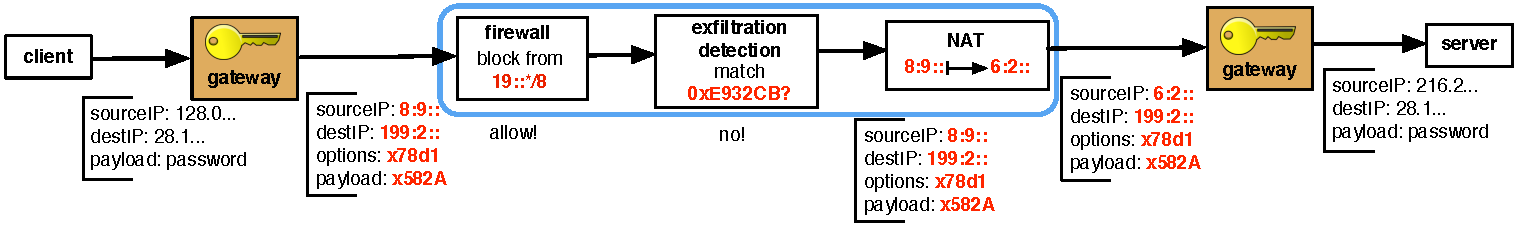
\includegraphics[width=6.7in]{fig/packetpath.pdf}
\caption{Example of packet flow through a few middleboxes. Red in bold indicates encrypted data. \label{fig:packetflow}}
\end{figure*}

To protect privacy, \sys \textit{encrypts all traffic} passing through the service provider (SP).
\sys encrypts the entire packet, including payloads and headers; the enterprise knows the contents of these packets but SP does not. \DIFaddbegin \DIFadd{One might ask why do we want to encrypt headers as well. Communication includes endpoints and contents, and both types of information should not be revealed. While contents are carried in the packet payloads, information about endpoints are mostly in the headers. 
}\DIFaddend 

\sys also provides the cloud provider with a set of {\it encrypted rules}.
Typically, header policies like firewall rules are generated by a local network administrator. Hence, the gateway knows these rules, and these rules may or may not be hidden from the cloud.
DPI and filtering policies on the other hand may be private to the enterprise (as in exfiltration policies), known by both parties (as in  public blacklists), or known only by the cloud provider (as in  patented malware signatures).
We discuss how rules are encrypted, generated and distributed given these different trust settings in \S\ref{sec:rulenc}.

As in Fig.~\ref{fig:sys-overview}, the gateway has a secret key $k$; in the setup with two gateways, they share
the same secret key. 
At setup time, the gateway generates the set of encrypted rules using $k$ and provides them to SP.
Afterwards, the gateway encrypts all traffic going to the service provider using \sys's encryption schemes.
The middleboxes at SP process  encrypted traffic, comparing the traffic against the encrypted rules. 
After the processing, the middleboxes
will produce encrypted traffic which SP sends back to the gateway. The gateway decrypts the traffic using the key $k$.

Throughout this process, middleboxes at SP handle only encrypted traffic and never access the decryption key. 
On top of \sys's encryption, the gateway can use a secure tunneling protocol, such as SSL or IPSec to secure the communication to SP.




\noindent\textbf{Packet encryption.}
The key idea is to encrypt packets {\it field-by-field}: \eg{}  an encrypted packet will contain a source address that is an encryption of the original packet's source address. We ensure that the encryption has the same size as the original data, and place any additional encrypted information or metadata in the options field of a packet. 

\sys uses three encryption schemes to protect the privacy of each field while allowing comparison against encrypted rules at the cloud: 

\begin{myitemize}
\item Traditional AES: provides strong security and no computational capabilities
\item KeywordMatch:  allows the provider to detect if an encrypted value in the packet is equal to an encrypted rule; does not allow two encrypted values to be compared to each other
\item \DIFdelbegin \DIFdel{RangeMatch}\DIFdelend \DIFaddbegin \DIFadd{PrefixMatch}\DIFaddend : allows the provider to detect whether or not an encrypted value lies in a range of rule values -- e.g. addresses in 128.0.0.0/24 or ports between 80-96.
\end{myitemize}
We discuss these cryptographic algorithms in \S\ref{sec:buildingblocks}.

For example, we encrypt IP addresses using \DIFdelbegin \DIFdel{RangeMatch}\DIFdelend \DIFaddbegin \DIFadd{PrefixMatch}\DIFaddend . This allows, e.g., a firewall to check whether the packet's source belongs to a prefix known to be controlled by a botnet -- but without learning what the actual source IP address is.
We choose which encryption scheme is appropriate for each field based on a high level classification of middlebox capabilities.
Table~\ref{tbl:mbreqs} shows a list of all middleboxes supported by typical outsourcing deployments~\cite{aplomb} and their processing requirements.
We classify these middleboxes as operating only over L3/L4 headers, operating only over L3/L4 headers and HTTP headers, or operating over all data including arbitrary fields in the connection bytestream (DPI).
We revisit them in detail in \S\ref{sec:mbs}.

All encrypted packets are converted to IPv6 because our \DIFdelbegin \DIFdel{RangeMatch }\DIFdelend \DIFaddbegin \DIFadd{PrefixMatch }\DIFaddend scheme requires 128 bits to encode an encrypted IP address  -- and because we expect more and more service providers to be moving to IPv6 by default in the future.
This is a trivial requirement as it is easy to convert from IPv4 to IPv6 (and back) at the gateway~\cite{siit}; clients may continue using IPv4 and the tunnel connecting the gateway to the provider may be either v4 or v6.

{\bf Example.} Fig.~\ref{fig:packetflow} shows the end-to-end flow of a packet through three example middleboxes in the cloud, each middlebox operating over an encrypted field.  
First,  the gateway encrypts the packet as explained above. The packet passes through the firewall which tries to match the encrypted information from the header against its encrypted rule, and decides to allow the packet. Next, the exfiltration device checks for any suspicious (encrypted) strings in data encrypted for DPI and not finding any, it allows the packet to continue to the NAT. The NAT maps the source IP address to a different IP address. Back at the gateway, the gateway decrypts the packet. 

\subsection{Architectural Implications} 
\label{sec:bbarch}
%%%End the discussion wiht BB here.
%%% DO NOT DELETE.

As mentioned, when compared to BlindBox, \sys provides new cryptography and system designs to support  more general middleboxes --  it turns out that, on top of these, the architectural setting of \sys provides additional benefits, which we can now explain.


%new encryption scheme and a new system design that enables a complete set of middleboxes, 
%So far, we have described the overall architecture of \sys without discussing how the encryption or middleboxes themselves are implemented.
%It is worth pausing here to discuss how this architecture itself can improve BlindBox, although it only supports DPI.
%
The first benefit is increased performance. In BlindBox, two arbitrary user endpoints communicate over a modified version of HTTPS. BlindBox requires 97 seconds to perform the initial handshake, which results in the encryption of the rules. 
This exchange must be performed for every new connection in BlindBox because each session is between two new endhosts with a per-connection key.
However, in the \sys context, this exchange can be performed just once at the gateway because the connection between the gateway and the cloud provider is long-lived. Consequently, there is no per-connection overhead. 
%, after which the same encrypted rules can be reused for all clients; this key is safe to re-use because it is private to the gateway.
%Most importantly, this architecture provides practical performance, where the BlindBox context imposed a prohibitive per-connection overhead.


The second benefit is increased deployability. In \sys, the gateway encrypts traffic where in BlindBox the end hosts do. Hence, deployability improves because the end hosts do not need to be modified.

Finally, security improves in the following way.
BlindBox has two security models: a stronger one to detect rules that are `exact match' substrings, and a weaker one to detect rules that are regular expressions. The more rules there are, the higher the per-connection setup cost is. 
Since there is no per-connection overhead  in \sys, we can afford having more rules. 
Hence, we convert many regular expressions to a set of exact-match strings. 
For example /hello[1-3]/ is equivalent to exact matches on "hello1", "hello2", "hello3".
Nonetheless, many regular expressions remain too complex to do so -- if the set of potential exact matches is too large, we leave it as a regular expression.
As we show in \S\ref{sec:eval}, this approach halves the number of rules that require using the weaker security model, enabling more rules in the stronger security model. 

In the rest of the paper, we do not revisit these architectural benefits, but focus  on \sys's new capabilities that allow us to outsource a {\it complete} set of middleboxes.

%!TEX root = mb.tex



\section{Cryptographic Building Blocks}
\label{sec:buildingblocks}

In this section we present the building blocks \sys relies on.
Symmetric-key encryption (based on AES) is well known, and we do not discuss it here. Instead, we briefly discuss KeywordMatch (introduced by~\cite{blindbox}, to which we refer the reader for details) and more extensively discuss \DIFdelbegin \DIFdel{RangeMatch}\DIFdelend \DIFaddbegin \DIFadd{PrefixMatch}\DIFaddend , a new cryptographic scheme we designed for this setting.
When describing these schemes we refer to the encryptor as the gateway whose secret key is $k$ and to the entity computing on the encrypted data as the service provider (SP).


\subsection{KeywordMatch}\label{s:kwmatch}


KeywordMatch allows detecting if an encrypted keyword matches an encrypted data item by equality.
For example, given an encryption of the keyword ``malicious'', and a list of encrypted strings  [$\Enc$(``alice''), $\Enc$(``malicious''), $\Enc$(``alice'')], SP can  detect that the keyword matches the second string. 
For  this, we use a searchable encryption scheme~\cite{song:search, blindbox}.
Using this scheme, the gateway can encrypt a value $v$ into $\enc(v)$ and a rule $r$ into $\encr$ and SP can detect if there is a match between $v$ \DIFdelbegin \DIFdel{an }\DIFdelend \DIFaddbegin \DIFadd{and }\DIFaddend $r$. 
 The security of searchable encryption is well studied~\cite{song:search, blindbox}: at a high level,  given a list of encrypted strings, and an encrypted keyword, SP does not learn anything about the encrypted strings, other than which strings match the keyword. 
 The encryption of the strings is {\em randomized}, so it does not leak whether two encrypted strings are equal to each other, unless, of course, they both match the encrypted keyword. 
  We use the technique from~\cite{blindbox} \DIFaddbegin \DIFadd{and hence do not elaborate on it}\DIFaddend .

%!TEX root = mb.tex

%\section{Building block: Range match}
%An important operation over an encrypted packet is to determine if an encrypted field in the packet falls in an encrypted range.
%We will use the firewall as an example. 
%Consider the following firewall rule:
%
%Constructing an encryption scheme that allows checking if an encrypted value is in an encrypted range, has been a challenge in the applied cryptography community. The reason is that ..
%
%\begin{itemize}
%\item preserve the order between Encryptd values
%\item candidate: OPE
%\item candidate: mOPE
%\item So none of the existing schemes are satisfactory. A new scheme \RM.
%\end{itemize}
%
%\RM applies to cases when we know an upper bound on the values encrypted with OPE and this is a small number of values (say, less than 10,000).
%
%The small number of values permits us to improve in two ways over mOPE [1]
%No more interaction. We store the tree in mOPE on the gateway (client) side, which means that the gateway can compute a new encryption by itself without help from service provider. The storage at the gateway will remain small.
%Rare updates to ciphertexts. We can space out the ciphertexts of the values encrypted sufficiently. 
%
%This also enjoys a stronger security than OPE! It leaks less than order.
%The reason is that, the server does not learn the order between the values in packets, and only whether they map between two values in the rules. 
%
%this one is new
%
%discuss 
%
%would be good to explain the challenge from the 
%
%\todo{a more interesting name to the scheme}
%
%prefix gets mapped into interval, at most a certain number
%
%talk about building certain data structures that all works the same
%
%firewall need not change 

\subsection{\DIFdelbegin \DIFdel{RangeMatch }\DIFdelend \DIFaddbegin \DIFadd{PrefixMatch}\DIFaddend } \label{sec:range}

\DIFaddbegin \todo{what is the size of $\slen$, $\plen$, and $\ptlen$? we need to be consistent in all the examples}


\DIFaddend Many middleboxes perform detection over \DIFdelbegin \DIFdel{a }\DIFdelend {\it \DIFdelbegin \DIFdel{range}\DIFdelend \DIFaddbegin \DIFadd{prefixes}\DIFaddend } \DIFaddbegin \DIFadd{or }{\it \DIFadd{ranges}} \DIFaddend of port numbers or IP addresses \DIFdelbegin \DIFdel{. }\DIFdelend \DIFaddbegin \DIFadd{(i.e. packet classification). }\DIFaddend For example, a network administrator might wish to block access to all servers hosted by MIT, in which case the administrator would block access to the prefix 18.0.0.0/8, \ie{}, 18.0.0.0-18.255.255.255. \DIFdelbegin \DIFdel{RangeMatch }\DIFdelend \DIFaddbegin \DIFadd{PrefixMatch }\DIFaddend enables a middlebox to tell whether an IP address $v$ \DIFdelbegin \DIFdel{lines }\DIFdelend \DIFaddbegin \DIFadd{lies }\DIFaddend in between a range $[s_1, e_1]$, where $s_1$ = 18.0.0.0 and $e_1$ = 18.255.255.255; however, the middlebox does not learn the values of $v$, $s_1$, or $e_1$. Unlike KeywordMatch\DIFdelbegin \DIFdel{(or AES), RangeMatch }\DIFdelend \DIFaddbegin \DIFadd{, PrefixMatch }\DIFaddend is a new scheme we designed specifically for our setting.

One might ask whether \DIFdelbegin \DIFdel{RangeMatch }\DIFdelend \DIFaddbegin \DIFadd{PrefixMatch }\DIFaddend is necessary, or one can instead employ KeywordMatch using the same expansion technique we used for some (but not all) regexps in \S\ref{sec:bbarch}. 
To detect whether an IP address is in a range, one could enumerate all IP addresses in that range and perform an equality check. However, the overhead of using this technique for common network ranges such as firewall rules is prohibitive.
For our own department network, doing so would convert our IPv6 and IPv4 firewall rule set of only 97 range-based rules to $2^{238}$ exact-match only rules; looking only at IPv4 rules would still lead to 38M exact-match rules.
Hence, to perform typical middlebox behaviors {\it in practice}, we require a \DIFdelbegin \DIFdel{RangeMatch }\DIFdelend \DIFaddbegin \DIFadd{PrefixMatch }\DIFaddend scheme which is more efficient.




\DIFdelbegin \subsubsection{\DIFdel{Requirements}}
%DIFAUXCMD
\addtocounter{subsubsection}{-1}%DIFAUXCMD
\DIFdel{The functionality of our RangeMatch scheme is to encrypt }\DIFdelend \DIFaddbegin \mypara{Functionality}
\DIFadd{PrefixMatch encrypts }\DIFaddend a set of ranges \DIFdelbegin \DIFdel{$[s_1, e_1]$, $\dots$, $[s_n, e_n]$ into $[\Enc(s_1)$, $\Enc(e_1)]$, $\dots$, $[\Enc(s_n)$,  $\Enc(e_n)]$, and }\DIFdelend \DIFaddbegin \DIFadd{or prefixes $P_1, \dots, P_n$ into a set of encrypted prefixes. For each $P_i$, there is one or more corresponding encrypted prefixes: $\ov{P}_{i,1} \dots, \ov{P}_{i, n_i}$.  Additionally, \pmatch{} encrypts }\DIFaddend a value $v$ into \DIFdelbegin \DIFdel{$\Enc(v)$, such that anyone with access to these encryptions can determine in which range $v$ lies, while not learning the  values of $s_1$, $e_1$,  
$\dots$, $s_n$, $e_n$, and $v$.
For concreteness, we explain our scheme by considering $v$, $e_i$ }\DIFdelend \DIFaddbegin \DIFadd{an encrypted value $\ov{v}$. These encryptions have the  property that, for all $i$,  
%DIF > 
}\[  \DIFadd{v \in P_i  \Leftrightarrow \ov{v} \in \ov{P}_{i, 1} \cup \dots \cup \ov{P}_{i, n_i}. }\]
%DIF > 
\DIFadd{In other words, the encryption preserves prefix matching.
}

\DIFadd{For example, suppose that encrypting $P$ = 18.0.0.0/8 (translated to 0::ffff:18.0.0.0/104 in IPv6) results in one encrypted prefix $\ov{P}$ = 1234::/16, encrypting $v_1$ = 18.0.0.2 (0::ffff:18.0.0.2) results in  
 $\ov{v_1}$ = 1234:db80:85a3:0:0:8a2e:37a0:7334, and encrypting $v_2$ = 19.0.0.1 (0::ffff:19.0.0.1) results in 
$\ov{v_2}$ = dc2a:108f:1e16:992e:a53b:43a3:00bb:d2c2. We can see that $\ov{v_1} \in \ov{P}$ }\DIFaddend and \DIFdelbegin \DIFdel{$s_i$ as IP addresses (although it can be used for encrypting ports too) }\DIFdelend \DIFaddbegin \DIFadd{$\ov{v_2} \notin \ov{P}$}\DIFaddend . 

\DIFaddbegin \todo{some of the below might have to move somewhere else}
\DIFaddend Our goal in designing \DIFdelbegin \DIFdel{RangeMatch }\DIFdelend \DIFaddbegin \DIFadd{PrefixMatch }\DIFaddend was for it to be both efficient/fast {\em and} to provide strong security.



In terms of performance, both encryption (performed at the gateway) and detection (performed at the middlebox) should be practical for typical middlebox line rates.
Our \DIFdelbegin \DIFdel{RangeMatch encrypts in $< 3\mu$}\DIFdelend \DIFaddbegin \DIFadd{PrefixMatch encrypts in $< 0.5\mu$}\DIFaddend s per value (we evaluate in \S\ref{sec:eval}).
Our design performs comparison between encrypted values and an encrypted rule (performed at the middlebox) using only on normal $\leq$/$\geq$ operators; hence it is compatible with existing classification algorithms such as tries, area-based quadtrees, FIS-trees, or hardware-based algorithms~\cite{packet_classif}.

For security, we require that the encryption scheme not leak $v$ to SP.
SP must not learn anything about $v$ other than \DIFdelbegin \DIFdel{what interval }\DIFdelend \DIFaddbegin \DIFadd{which encrypted rule }\DIFaddend it matches to. 
In particular, even if \DIFaddbegin \DIFadd{both tuples }\DIFaddend $v_1$ and $v_2$ match the same \DIFdelbegin \DIFdel{range}\DIFdelend \DIFaddbegin \DIFadd{rule}\DIFaddend , SP should not learn \DIFdelbegin \DIFdel{their order .
RangeMatch }\DIFdelend \DIFaddbegin \DIFadd{the order between them for each field of the tuple.
PrefixMatch }\DIFaddend also provides a level of security for the endpoints of \DIFdelbegin \DIFdel{a range :
 $e_1$, $s_1$}\DIFdelend \DIFaddbegin \DIFadd{the $j$-th range of rules:
 $s_{1j}$, $e_{1j}$}\DIFaddend , $\dots$, \DIFdelbegin \DIFdel{$e_n$, $s_n$}\DIFdelend \DIFaddbegin \DIFadd{$s_{nj}$, $e_{nj}$}\DIFaddend . SP should not learn their values, \DIFdelbegin \DIFdel{but  SP is allowed to }\DIFdelend \DIFaddbegin \DIFadd{and SP should not }\DIFaddend learn the order relation of the intervals\DIFdelbegin \DIFdel{(in fact, in many setups, the intervals are public information such as blacklists, or provided by the SP)}\DIFdelend . To the best of our knowledge, \DIFdelbegin \DIFdel{RangeMatch }\DIFdelend \DIFaddbegin \DIFadd{PrefixMatch }\DIFaddend is the only practical encryption scheme that achieves these security guarantees.

Although \DIFdelbegin \DIFdel{RangeMatch }\DIFdelend \DIFaddbegin \DIFadd{PrefixMatch }\DIFaddend has a similar functionality to order-preserving encryption such as BCLO~\cite{boldyreva:ope} or mOPE~\cite{popa:mope}, neither meets our security requirement (because they leak the ordering between encrypted values, not just whether they match a range) or provides the performance necessary for packet processing (as we show in \S\ref{sec:eval}).

%DIF < \begin{CompactEnumerate}[leftmargin=*]
%DIF < \item  {\em be fast}: the throughput of encryption should be not much lower than network throughput. In particular, the scheme should preserve the ability to use {\em existing fast packet matching algorithms}, such as  various kinds of tries, area-based quadtrees, FIS-trees, or hardware-based algorithms~\cite{packet_classif}.  All of these rely on the ability of SP  to compute ``>'' between $v$ and the endpoints of an interval,
%DIF < hence the encryption scheme should preserve this property. 
\DIFdelbegin %DIFDELCMD < 

%DIFDELCMD < %%%
%DIF < \item {\em provide strong security}: The encryption scheme should not leak $v$, $e_1$, $s_1$, $\dots$, $e_n$, $s_n$ to SP.
%DIF < Ideally, SP does not learn anything about $v$ other than what interval it matches to. In  particular, even if $v_1$ and $v_2$ match the same range, SP should not learn their order. SP is allowed to learn the order relation of the intervals (in fact, in many setups, SP provides the intervals). \label{req:sec}
%DIFDELCMD < 

%DIFDELCMD < %%%
%DIF < \item {\em be deterministic}: To integrate with NAT and to enable middleboxes to piece together packets from the same flow, each value should get  consistently  the same encryption. Any changes in the encryption assigned should happen rarely.  \label{req:injective}
%DIFDELCMD < 

%DIFDELCMD < %%%
%DIF < \item {\em be format-preserving}: The encryption should have the same format as the data. Concretely, an encrypted IP address should look like an IP address.  This property is important to avoid changing the packet header structure, which would be a hurdle to adoption. 
%DIF < \end{CompactEnumerate}
%DIFDELCMD < 

%DIFDELCMD < %%%
\DIFdelend \subsubsection{Scheme} 
\label{sec:rmscheme}
%DIF < We explain the scheme based on encryption IP addresses for a firewall and source IP addresses in packets, although the scheme is used in encryption other fields too, as explained in Sec.~\ref{xx}.

\DIFdelbegin \DIFdel{To encrypt the endpoints of intervals, we sort them, and choose as their encryptions values equally distributed in the domain space in a way that preserves the order of the endpoints . }\DIFdelend \DIFaddbegin \begin{figure}[t]
  \centering
  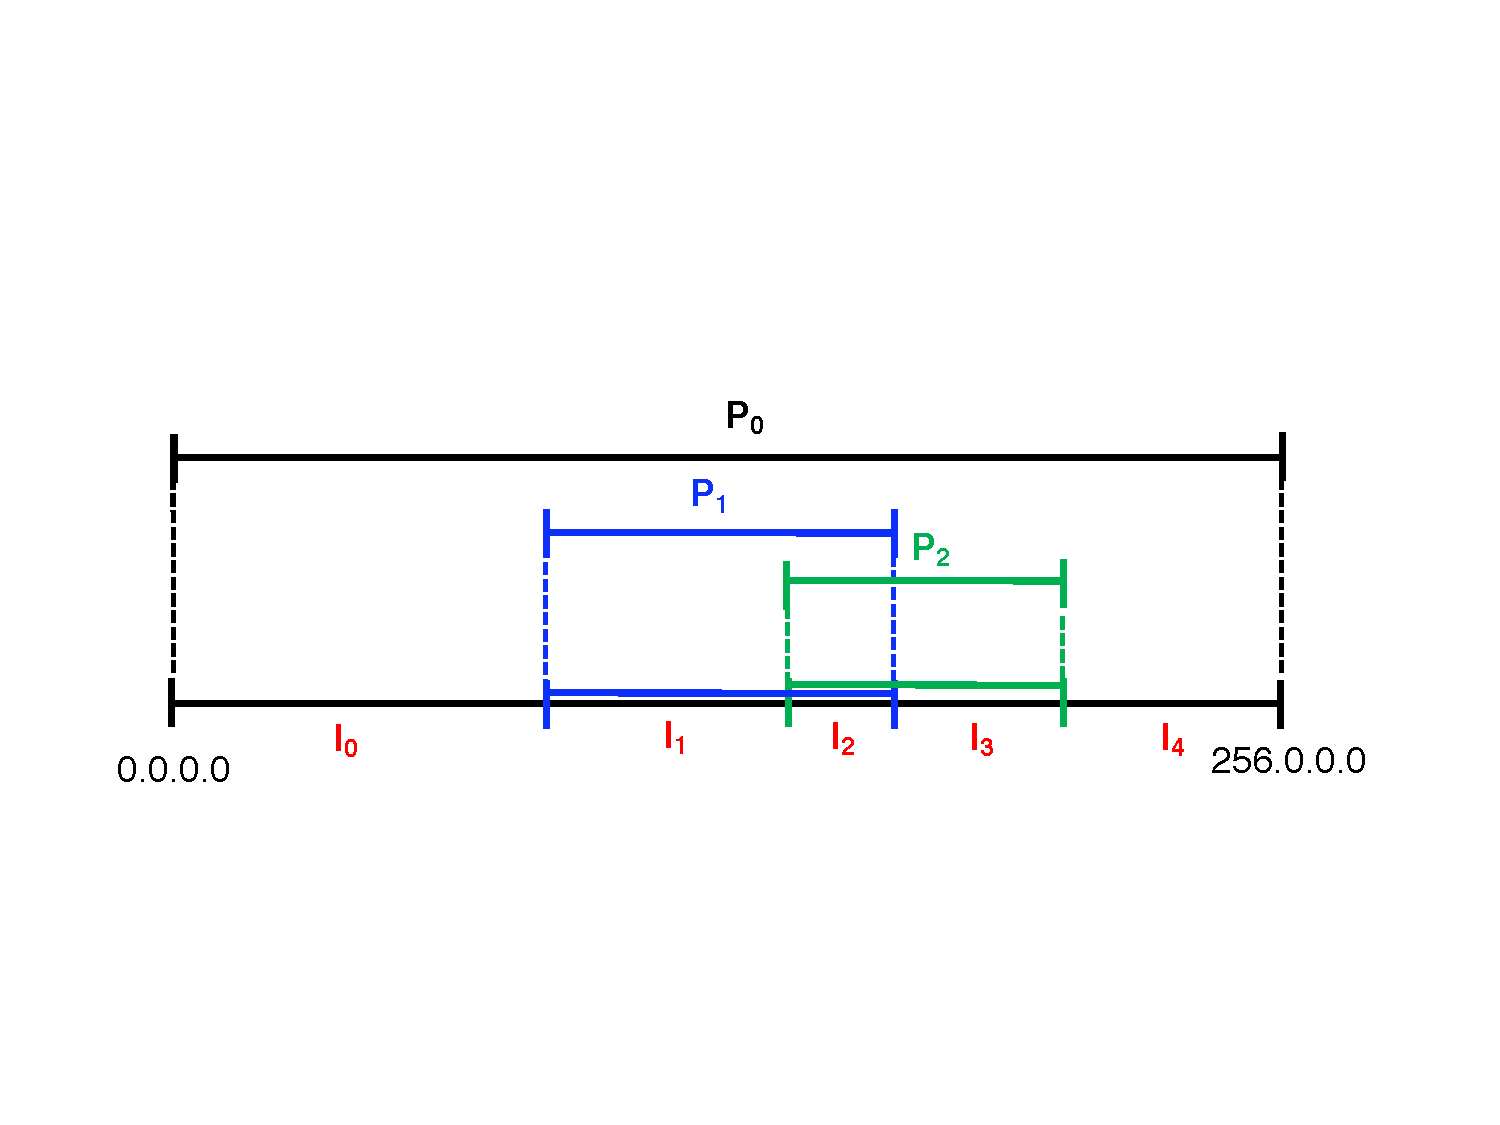
\includegraphics[width=3in]{fig/rangeopts3.pdf}
  \caption[]{\DIFaddFL{Example of prefix encryption with PrefixMatch.}\label{fig:rangeopts3}}
\end{figure}

\DIFadd{We now explain how PrefixMatch works. To illustrate the protocol, we use IP addresses, but the scheme works with 
ports and other value domains too.
}



\mypara{Prefixes/ranges encryption} \DIFadd{\pmatch{} takes as input a set of prefixes or ranges $P_1 = [s_1, e_1], \dots, P_n$, 
whose endpoints have size $\ptlen$ bits. \pmatch{} encrypts each prefix or range into a set of encrypted prefixes: these prefixes are $\plen$ bits long with a suffix of $\slen = \ptlen - \plen$. The selection of $\plen$ depends on the number of intervals (introduced below). }\DIFaddend For example, \DIFdelbegin \DIFdel{the encryption of the intervals 127.0.0.0/8 }\DIFdelend \DIFaddbegin \DIFadd{when $\plen = 16$, the maximum number of intervals can be 65536, which is sufficient for a typical rule set.
}

\DIFadd{Consider all the endpoints $s_i$ }\DIFaddend and \DIFdelbegin \DIFdel{172.16.0.0/16, is }%DIFDELCMD < [%%%
\DIFdel{51.0.0.0, 102.0.0.0}%DIFDELCMD < ] %%%
\DIFdel{and }%DIFDELCMD < [%%%
\DIFdel{153.0.0.0, 204.0.0.0}%DIFDELCMD < ]%%%
\DIFdel{.
This preserves the order of intervals but does not leak anything else}\DIFdelend \DIFaddbegin \DIFadd{$e_i$ laid out on an axis in increasing order as in Fig.~\ref{fig:rangeopts3}.
Add on this axis the endpoints of $P_0$, the smallest and largest possible values, $0$ and $2^{\ptlen}-1$.
Consider all the intervals formed by each consecutive pair of such endpoints}\DIFaddend . 

For \DIFdelbegin \DIFdel{now, consider that the gateway  maintains a mapping of each interval endpoint  to its encryption, called the }\DIFdelend \DIFaddbegin \DIFadd{example, consider Fig.~\ref{fig:rangeopts3}.  There are two prefixes to encrypt: $P_1$ and $P_2$. PrefixMatch computes intervals $I_0, \dots, I_4$.
}

\DIFadd{PrefixMatch now assigns an encrypted prefix to each interval. Note that each interval belongs to a set of prefixes. Let $\prefixes(I)$ denote the prefix of interval $I$. For example, $\prefixes(I_2) = \{P_0, P_1, P_2\}$. The encrypted prefix is simply a }\DIFaddend {\em \DIFdelbegin \DIFdel{interval map}\DIFdelend \DIFaddbegin \DIFadd{random}\DIFaddend } \DIFdelbegin \DIFdel{.  The interval map also contains the points $- \infty$ and $+ \infty$, encrypted with 0.0.0.0 and 255.255.255.255. }\DIFdelend \DIFaddbegin \DIFadd{number of size $\plen$. Each interval gets a different random value, except for the intervals that belong to the same prefixes. For example, in Fig.~\ref{fig:rangeopts3}, intervals $I_0$ and $I_4$ receive the same random number.
}\DIFaddend 

\DIFdelbegin \DIFdel{When the gateway needs to encrypt an }\DIFdelend \DIFaddbegin \DIFadd{When an interval overlaps partially with another interval, it will have more than one encrypted prefix. For example, consider that $\plen = 16$, $I_1$ was assigned a random number of $0x123c$ and $I_2$ of $0xabcc$. The encryption of the prefix $P_1$ in Fig.~\ref{fig:rangeopts3} will be the pair ($123c::/14$, $abcc::/14$).
}

\DIFadd{Since the encryption is a random prefix, the encryption does not reveal the original prefix. Moreover, the fact that intervals pertaining to the same set of prefixes receive the same encrypted number hides where an encrypted value matches, as we discuss below. For example, for an }\DIFaddend IP address $v$ \DIFdelbegin \DIFdel{, the gateway first determines what  is the interval  }\DIFdelend \DIFaddbegin \DIFadd{that does not match either $P_1$ or $P_2$, the cloud provider will not learn whether it matches to the left or right of $P_1$ and $P_2$ because $I_0$ and $I_4$ receive the same encryption. The only information it learns about $v$ is that }\DIFaddend $v$ \DIFdelbegin \DIFdel{falls in (we discuss below what happens when more than one interval matches). It uses the interval map to determine the encryptions of the endpoints of this interval. Then, to encrypt }\DIFdelend \DIFaddbegin \DIFadd{does not match either $P_1$ or $P_2$. 
}

\DIFadd{We now present the EncryptPrefixes procedure, which works the same for prefixes or ranges.
}



\begin{framed}
\ALGORITHM{EncryptPrefixes}{proc:enc_prefixes}{$P_1$, $\dots$, $P_n$, $\plen$, $\ptlen$, $\slen$}{
\item Let $s_i$ and $e_i$ be the endpoints of $P_i$. \comment{$P_i = [s_i, e_i]$}
	\item Assign $P_0 \gets [0, 2^{\ptlen}-1]$
	\item Sort all endpoints in increasing order
	\item  Construct intervals $I_0, \dots, I_m$ from each pair of consecutive endpoints. Multiple equal endpoints form a unit interval. For each interval $I_i$, compute $\prefixes(I_i)$, the list of prefixes $P_{1}, \dots, P_{m_i}$ that contain   $I_i$. 
	\item Assign a distinct random value of size $\plen$ to each of $\ov{I_0}, \dots, \ov{I_m}$  
	\item For all $i, j$ with $i<j$ if the prefixes containing $I_i$ and $I_j$ are the same, set $\ov{I_j} \gets \ov{I_i}$
	\item The encryption of $P_i$ is $\ov{P_i} = \{\ov{I_j}/\plen, I_j \in \prefixes(P_i) \}$. The encrypted prefixes are output sorted by value (as a means of randomization).
	\item Output $\ov{P_1}, \dots,\ \ov{P_n}$ and the {\em interval map} [$I_i \rightarrow \ov{I_i}$] 
}
\end{framed}

\mypara{Value encryption}
\DIFadd{To encrypt a value }\DIFaddend $v$\DIFaddbegin \DIFadd{, PrefixMatch locates the one interval $I$ such that $v \in I$. $\ov{I}$ becomes the prefix of the encryption of $v$. This ensures that the encrypted $v$}\DIFaddend , \DIFdelbegin \DIFdel{it chooses a random value in this interval.  
}\DIFdelend \DIFaddbegin \DIFadd{$\ov{v}$, matches $\ov{I}/\plen$. The suffix of $v$ is chosen at random. The only requirement is that it is deterministic. }\todo{link}
\DIFadd{Hence, the suffix is chosen based on a pseudorandom function that $\prf^{\slen}$ seeded in a given seed  $\seed$.  
}



\DIFaddend For example, if $v$ is 127.0.0.1 \DIFaddbegin \DIFadd{(0::ffff:127.0.0.1), and the assigned prefix for the matched interval is $abcd::/16$}\DIFaddend , a possible encryption given the ranges encrypted above is \DIFdelbegin \DIFdel{78.124.24.85. The encryption }\DIFdelend \DIFaddbegin \DIFadd{$Enc(v) = abcd:ef01:2345:6789:abcd:ef01:2345:6789$. Note that the ecryption }\DIFaddend does not retain any information about $v$ other than the \DIFdelbegin \DIFdel{range it is }\DIFdelend \DIFaddbegin \DIFadd{interval it matches }\DIFaddend in. In particular, \DIFdelbegin \DIFdel{for }\DIFdelend two values $v_1$ and $v_2$ that match the same interval, their order can be arbitrary. Thus, \DIFdelbegin \DIFdel{this satisfies the security requirement above}\DIFdelend \DIFaddbegin \DIFadd{PrefixMatch does not reveal order}\DIFaddend .

\DIFdelbegin %DIFDELCMD < \begin{figure}[t]
%DIFDELCMD <   \centering
%DIFDELCMD <   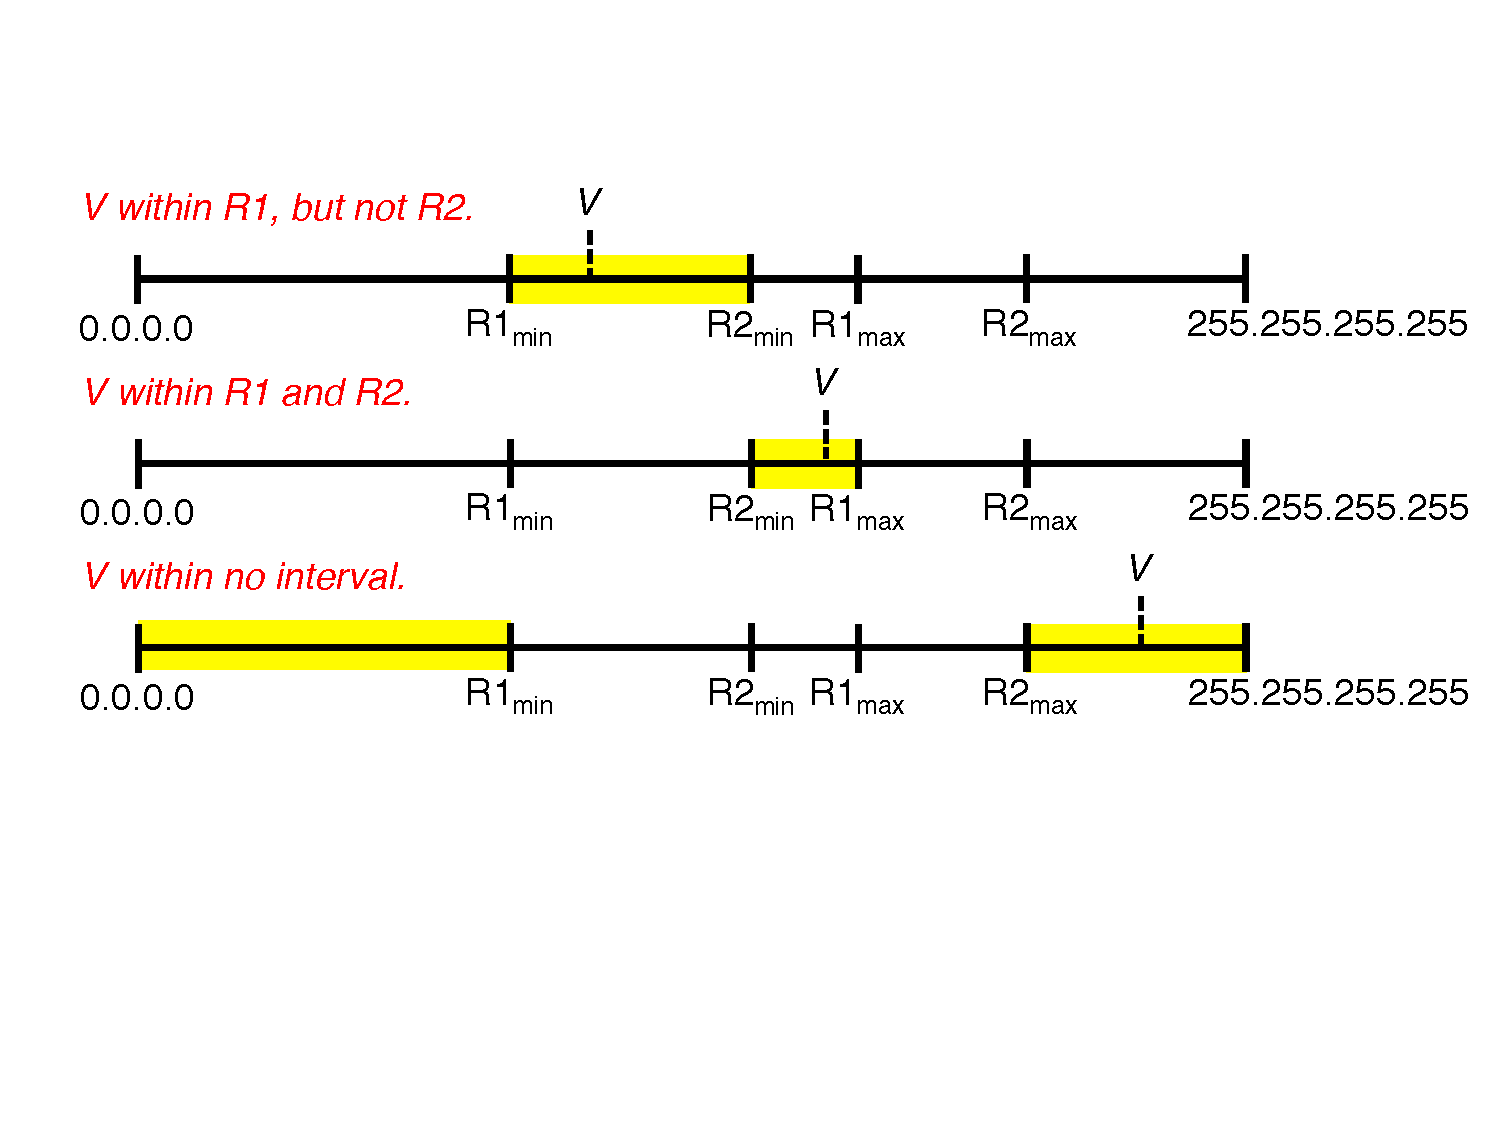
\includegraphics[width=3in]{fig/rangeopts.pdf}
%DIFDELCMD <   %%%
%DIFDELCMD < \caption[]{%
{%DIFAUXCMD
\DIFdelFL{Possible RangeMatch encryption values: the yellow areas indicate the intervals from which $v$ is sampled at random.}%DIFDELCMD < \label{fig:rangeopts}%%%
}
%DIFAUXCMD
%DIFDELCMD < \end{figure}
%DIFDELCMD < %%%
\DIFdel{To generalize this insight, we need to specify how to encrypt $v$ when $v$ fits in multiple intervals or in no interval at all. Figure~\ref{fig:rangeopts} illustrates how $v$ is mapped depending on whether it maps to zero, one, or both of ranges $R1$ and $R2$; we formalize this as follows. 
}\DIFdelend \DIFaddbegin \begin{framed}
\ALGORITHM{EncryptValue}{proc:enc_value}{$\seed$, $v$, $\slen$, interval map}{
\item Run binary search on interval map to locate the interval $I$ such that $v \in I$.
\item Lookup $\ov{I}$ in the interval map.
\item Output 
\begin{equation}
\Enc(v) = \ov{I} \Vert \prf_\seed^\slen(v)
\end{equation}
}
\end{framed}
\DIFaddend 


\DIFdelbegin \DIFdel{To achieve the desired security, we find the interval $I$ (which may consist of many sub-intervals, }%DIFDELCMD < \eg{} %%%
\DIFdel{when $v$ matches neither $R1$ or $R2$ in Fig.
~\ref{fig:rangeopts}) inside which $v$ should be mapped at random. The equation for $I$ is as follows. Consider the intervals }%DIFDELCMD < {\em %%%
\DIFdel{inside}%DIFDELCMD < } %%%
\DIFdel{which $v$ falls, and let $I_0, I_1, \dots, I_{n_I}$ be their encryptions.
We always include the interval $I_0 = [0.0.0.0, 255.255.255.255]$. Now consider the intervals }%DIFDELCMD < {\em %%%
\DIFdel{outside}%DIFDELCMD < } %%%
\DIFdel{of which $v$ falls and let $O_1, \dots, O_{n_O}$ be their encryptions. Then, to provide our desired security goal, $v$ should be chosen at random from the interval  
}\begin{displaymath}
 \DIFdel{I = I_0 \cap I_1 \cap ... \cap I_{n_I} - (O_1 \cup \dots \cup O_2). \label{eq:randominterval}
 }\end{displaymath}
%DIFAUXCMD
\DIFdelend %DIF > \begin{figure}
%DIF >   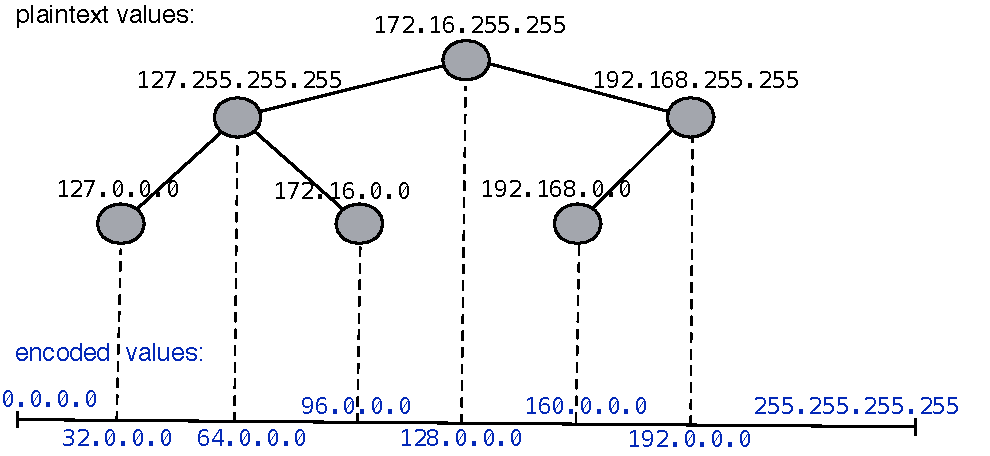
\includegraphics[width=3.25in]{fig/tree}
%DIF >   \caption{\label{fig:tree} PrefixMatch tree. The values of nodes in the tree are the %unencrypted IP addresses, and the blue values on the horizontal axis are their encryptions. }
%DIF > \end{figure}

\DIFdelbegin \DIFdel{To support middleboxes like NATs -- which require that every time a value for the same connection is encrypted, it returns the same value -- we need to generate the random encryptions using a deterministic function. Importantly, this value should always be the same }%DIFDELCMD < {\it %%%
\DIFdel{within}%DIFDELCMD < } %%%
\DIFdel{the same connection, but across unique connections it should be different. For this, we use a pseudorandom function~\mbox{%DIFAUXCMD
\cite{GoldreichVol1}}%DIFAUXCMD
, $\prf$. 
Let $\prf$ be a function $\prf^{n}(v)$, mapping }\DIFdelend \DIFaddbegin \mypara{Comparing encrypted values against rules}
\DIFadd{Determining if an encrypted value matches an encrypted prefix is straightforward: the encryption preserves the prefix.
Hence, a regular packet classification can be run at the firewall with no modification. Comparing different encrypted values for order that match the same prefix is meaningless, and returns a random value.
}




\subsubsection{\DIFadd{Security Guarantees}}

\DIFadd{\pmatch{} hides the endpoints of ranges or the prefixes encrypted with EncryptPrefixes and it does not reveal the values encrypted with EncryptValue. \pmatch{} reveals only matching information between values and prefixes to enable functionality at the cloud provider.  For every subset of prefixes out of $P_1, \dots, P_m$, the cloud provider learns if these overlap and whether an encrypted value }\DIFaddend $v$ \DIFdelbegin \DIFdel{to a random value in }\DIFdelend \DIFaddbegin \DIFadd{matches them. In particular, }\DIFaddend the \DIFdelbegin \DIFdel{interval 1\ldots n.
}\DIFdelend \DIFaddbegin \DIFadd{cloud provider does not learn the order of encrypted values $\Enc(v)$ or the order of the prefixes. Hence, PrefixMatch is significantly more secure than order-preserving encryption.
}\DIFaddend 

%DIF > 
\DIFaddbegin \DIFadd{Since the encryption is seeded in a per-connection identifier, correlation attacks between different flows are not possible. 
In particular, even though EncryptValue is deterministic, the encryption of the same IP address in different flows will be different because the seed differs per flow.
}\todo{the above sentence needs some context}

\DIFaddend We \DIFaddbegin \DIFadd{formalize and prove the security guarantees of \pmatch{} in our extended paper. 
}

\subsubsection{\DIFadd{Implementing PrefixMatch in the Gateway}}
\label{sec:tree}

\todo{THIS  SUBSECTION IS WORK IN PROGRESS}


\DIFadd{To encrypt a value with EncryptValue, we }\DIFaddend seed $\prf$ in \DIFdelbegin \DIFdel{$q$}\DIFdelend \DIFaddbegin \DIFadd{$\seed$}\DIFaddend , a function of both the key and hash of the \DIFdelbegin \DIFdel{5-tuple connection header ($q = \prf_k(\text{conn})$). Let $|I|$ be the size of the interval $I$. 
Then, the encryption of $v$ is the $\mathsf{index}$-th element in $I$, where $\mathsf{index}$ is 
}\begin{displaymath}
\DIFdel{\mathsf{index}(v) = \prf_{q}^{|I|}(v) 
}\end{displaymath}
  %DIFAUXCMD
\DIFdelend \DIFaddbegin \DIFadd{tuple being encrypted ($\seed = \prf_k(\text{(u, v)})$). }\DIFaddend Note that, in the system setup with two gateways, the gateways generate the same encryption because they share $k$.  

\DIFaddbegin \DIFadd{The scheme supports NATs -- which require that every time a value for the same connection is encrypted, it returns the same value. It generates a random encryption using a deterministic function. 
}

\DIFaddend When encrypting IP addresses, we do not want two different IP addresses to map to the same encryption (which would break the NAT). Fortunately, the probability that two IP addresses get assigned to the same encryption is negligibly low for IPv6.  The reason is that each interval of \DIFdelbegin \DIFdel{encryptions }\DIFdelend \DIFaddbegin \DIFadd{prefixes }\DIFaddend is large because we distributed the \DIFdelbegin \DIFdel{endpoint encryptions }\DIFdelend \DIFaddbegin \DIFadd{endpoints }\DIFaddend evenly and because there is a small number of such endpoints in a realistic setting (e.g., a firewall has less than 100,000 rules). Suppose we have $n$ distinct rules, $m$ flows and a $w$-bit space, \DIFdelbegin \DIFdel{the }\DIFdelend \DIFaddbegin \DIFadd{with the assumption of uniformly distributed flows, the }\DIFaddend probability of getting collision is approximately 
\DIFdelbegin \DIFdel{$1-e^\frac{-m^2 (n+1)}{2^{w+1}}$. }\DIFdelend \DIFaddbegin 

\begin{equation}
\DIFadd{1 - e^\frac{-m^2 (2n+1)}{2^{w+1}}
}\end{equation}

\todo{discuss how the gateway gives the seed -- is the choice of seed outside of the prefixmatch alg or inside?}
\todo{discuss security of ports clearly}

\DIFaddend Therefore, if $w=128$ (which is the case when we use IPv6), the probability is negligible in a normal setting. \DIFdelbegin \DIFdel{This probability is very low for IPv4, but not low enough that a collision will not happen in a large interval of time, so RangeMatch requires IPv6.
}\DIFdelend \DIFaddbegin \DIFadd{When encrypting ports, it is possible to get collisions since the port field is only 16-bit. However, this will not cause problem as long as the IP address does not collide, because NATs (and other middleboxes that require injectivity) considers both IP addresses and ports.
}\DIFaddend 

\DIFdelbegin %DIFDELCMD < \begin{figure}
%DIFDELCMD <   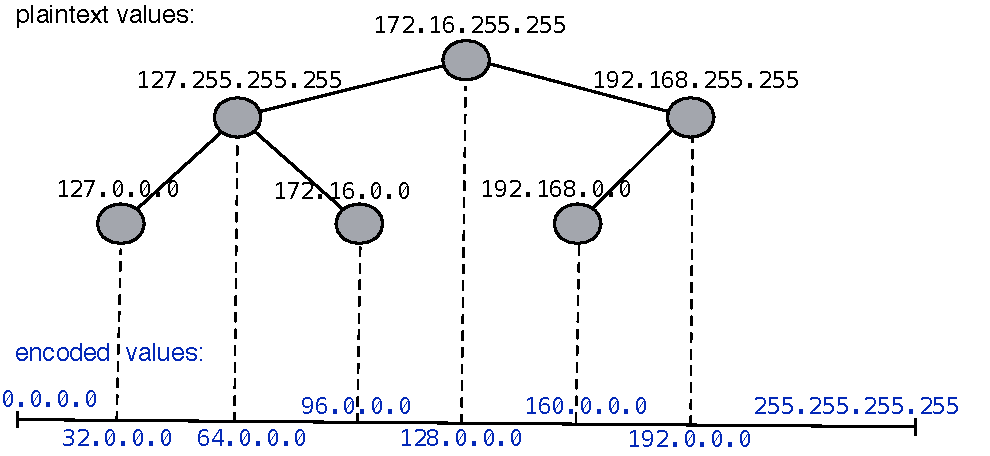
\includegraphics[width=3.25in]{fig/tree}
%DIFDELCMD <   %%%
%DIFDELCMD < \caption{%
{%DIFAUXCMD
%DIFDELCMD < \label{fig:tree} %%%
\DIFdelFL{Range match tree. The values of nodes in the tree are the unencrypted IP addresses, and the blue values on the horizontal axis are their encryptions. }}
%DIFAUXCMD
%DIFDELCMD < \end{figure}
%DIFDELCMD < %%%
\DIFdelend \DIFaddbegin \todo{make clear that it is seeded in this so IPs do not collide}
\DIFaddend 


\DIFdelbegin %DIFDELCMD < \noindent %%%
\textbf{\DIFdel{Comparing Encrypted Values against Rules.}}
%DIFAUXCMD
\DIFdel{The cloud can run ``$\ge$'' and ``$\le$" between any encrypted value $\enc(v)$ and an encrypted range endpoint $\enc(s)$ or $\enc(e)$, and will obtain a correct answer.
Computing $\enc(v_1) < \enc(v_2)$  between two encrypted values in the same range is meaningless, and returns a random value.
}\DIFdelend \DIFaddbegin \todo{need to discuss how the firewall puts prefix match in the prefix form, and adds /*}
\DIFaddend 

\DIFaddbegin \todo{remark for perfect security and tradeoff with work at the gateway}
\todo{does each rule become multiple rules?? explain who FW does with this, explain how many there are, need eval of this}
\todo{then in func you also need to clarfiy that it becomes more than one; this will leak about the prefixes what intersections they have!! even without fields matching}
\todo{and what does the firewall do?}


\todo{ I wonder how much of this section actually needs to move to the gateway section}

\todo{ need to discuss how the gateway chooses k for the encryptvalue -- the seed}

\DIFaddend \noindent \textbf{\DIFdelbegin \DIFdel{Adding new }\DIFdelend \DIFaddbegin \DIFadd{Updating }\DIFaddend ranges.}
Adding a new range \DIFdelbegin \DIFdel{could cause all the other ranges to shift. This might require middlebox rulesets to be entirely reconfigured. To avoid this, instead of assigning endpoints to evenly distributed encrypted values, we insert endpoints in a balanced search tree and assign encryptions based on the position in the tree as in Fig.~\ref{fig:tree}. When a new range is added, a tree rebalance operation may happen, which changes the encrypted values of a few endpoints. By using a scapegoat tree, the number of nodes that change position during rebalancing is amortized worst-case $O(\log n)$ where $n$ is the total number of nodes in the scapegoat tree}\DIFdelend \DIFaddbegin \DIFadd{or removing an existing range would affect the intervals it covers. Therefore, in the worst case $O(N)$ rules needs to be updated}\DIFaddend . 

\DIFdelbegin \subsubsection{\DIFdel{Implementing RangeMatch in the Gateway}}
%DIFAUXCMD
\addtocounter{subsubsection}{-1}%DIFAUXCMD
%DIFDELCMD < \label{sec:tree}
%DIFDELCMD < %%%
\DIFdelend \DIFaddbegin \todo{ and it has to be clear that to encrypt firewall rules at the gateway using the Prefix match, you need to go through each part of the rule and encrypt that; 
The gateway will use an instance of PrefixMatch for every field, destination IP, etc.
}
\todo{and need to discuss the prefix part}
\DIFaddend 

%DIF < Most encryption operations are relatively stateless -- they rely only on the key and the data. Using RangeMatch requires that the Rule Encryption component manage a tree of values for use at encryption time; we discuss how this tree is generated now.
%DIF < 
 \DIFaddbegin \todo{need to discuss the fact that they blowup here}


\DIFaddend The gateway stores the \DIFdelbegin \DIFdel{tree in Fig.~\ref{fig:tree}: for each node, it stores the unencrypted endpoint, whether it is the left or  right margin of an interval, and the other endpoint of the interval it is part of. It does not need to store the encryption of the endpoint because this is easy to derive from the position in the tree. 
The gateway keeps a small amount of state (in our implementation, about 200 bytes/range), %DIF < encryption the intervals
}\DIFdelend \DIFaddbegin \DIFadd{intervals and the mapping from intervals to prefixes for each field of the rules, }\DIFaddend and it maintains no state per IP address encrypted or per connection.

The gateway can use the following functions. \DIFdelbegin \DIFdel{EncryptRanges }\DIFdelend \DIFaddbegin \DIFadd{EncryptRules }\DIFaddend encrypts the initial \DIFdelbegin \DIFdel{ranges. Note that some ranges could consist of
one point only, namely $s = e$. 
}%DIFDELCMD < 

%DIFDELCMD < %%%
%DIF <  TO CUT TO REDUCE: put all these algorithms into one box
%DIF <  framed takes space around it, above it, below it 
%DIFDELCMD < 

%DIFDELCMD < \begin{framed}
%DIFDELCMD < \begin{algorithmic}[1]
%DIFDELCMD < 

%DIFDELCMD < \Procedure{EncryptRanges}{[$s_1$, $e_1$], $\dots$, [$s_n$, $e_n$]}
%DIFDELCMD <   \State %%%
\DIFdel{Build scapegoat tree on the values 
              $\{s_1, \dots, s_n\}$ 
              $\cup$ $\{e_1, \dots, e_n\}$ 
              $\cup$ $\{-\infty, \infty\}$.
  }%DIFDELCMD < \State %%%
\DIFdel{Assign an encryption $\enc(x)$ to each node $x$ in the tree:
  }%DIFDELCMD < \begin{itemize}
%DIFDELCMD <   \item %%%
\DIFdel{the root gets the middle of the IP range, $e$, 
  }%DIFDELCMD < \item %%%
\DIFdel{the node to the left of the root gets the middle of the interval to the left of $e$: ($e/2$),
  }%DIFDELCMD < \item %%%
\DIFdel{the right node gets the middle of the range
  to the right of $e$: ($3e/2$), and so on.
  }%DIFDELCMD < \end{itemize}
%DIFDELCMD < 

%DIFDELCMD <   \State \Return{[$\enc(s_1)$, $\enc(e_1)$], $\dots$, [$\enc(s_n)$, $\enc(e_n)$]}
%DIFDELCMD < \EndProcedure
%DIFDELCMD < 

%DIFDELCMD < \end{algorithmic}
%DIFDELCMD < \end{framed}
%DIFDELCMD < 

%DIFDELCMD < %%%
%DIF < EncryptValue encrypts the values to be matched against ranges.
%DIF < \begin{framed}
%DIF < \begin{algorithmic}[1]
%DIF < \Procedure{EncryptValue}{$v$}
%DIF <   \State Search the tree for $v$ to compute efficiently I as in Eq.~\ref{eq:randominterval}.
%DIF <   \State Compute $\mathsf{index}(v) = \prf_k(v)\ \mod\ |I|.$ 
%DIF <   \State Let $\enc(v)$ to be the $\mathsf{index}$-th element of $I$. 
%DIF <   \State \Return $\left(\enc(v), \IV, \aes_k(\IV, v)\right)$ for random $\IV$. 
%DIF < \EndProcedure
%DIF < \end{algorithmic}
%DIF < \end{framed}
%DIFDELCMD < 

%DIFDELCMD < %%%
\DIFdel{We described how to encrypt values matched against ranges in \S\ref{sec:rmscheme}}\DIFdelend \DIFaddbegin \DIFadd{rules. EncryptTuple encrypts packet header fields which are represented as a tuple}\DIFaddend ; it requires identifying \DIFdelbegin \DIFdel{set }\DIFdelend \DIFaddbegin \DIFadd{the interval }\DIFaddend $I$ \DIFdelbegin \DIFdel{of possible encryption values for each value. Here is how to }\DIFdelend \DIFaddbegin \DIFadd{for each field. We can }\DIFaddend compute $I$ efficiently \DIFdelbegin \DIFdel{. When searching for $v$ in the tree, the gateway
can identify the tightest enclosing interval }%DIFDELCMD < [%%%
\DIFdel{$p_1$, $p_2$}%DIFDELCMD < ] %%%
\DIFdel{in logarithmic time . 
 If $[p_1, p_2]$ are endpoints of the
same interval, then I = }%DIFDELCMD < [%%%
\DIFdel{$p_1$, $p_2$}%DIFDELCMD < ]%%%
\DIFdel{. Otherwise, move towards the left in the tree until you identify the first endpoint
$\ell_1$
that belongs to an interval $[\ell_1, \ell_2]$ enclosing $v$. Then, using the tree, scan $[\ell_1, \ell_2]$ and eliminate
any intervals not containing $v$. The gateway can precompute and store this interval for every two consecutive nodes in the tree.
}\DIFdelend \DIFaddbegin \DIFadd{in logarithmic time by doing a binary search. 
}\DIFaddend 




\DIFdelbegin \DIFdel{We now describe the procedure for AddRange which adds an interval (deleting an interval is similar).
These procedures modify the state at the gateway.
To add a range }%DIFDELCMD < [%%%
\DIFdel{$s$, $e$}%DIFDELCMD < ]%%%
\DIFdel{, the gateway inserts these values in the tree. 
If the tree needs to be rebalanced, for each endpoint that changed location in the tree, the gateway records the old and new encrypted value based
on the tree in a list $L$. Note that  the number of endpoints that change encryption is $O(\log n)$ amortized worst-case. 
The gateway then computes the encryption of $s$ and $e$ based on their location in the tree. 
It sends to SP $\enc(s)$ and $\enc(e)$ along with $L$. 
}\DIFdelend %DIF >  We now describe the procedure for AddRange which adds an interval (deleting an interval is similar). These procedures modify the state at the gateway. To add a range [$s$, $e$], the gateway inserts these values in the tree. If the tree needs to be rebalanced, for each endpoint that changed location in the tree, the gateway records the old and new encrypted value based on the tree in a list $L$. Note that  the number of endpoints that change encryption is $O(\log n)$ amortized worst-case. The gateway then computes the encryption of $s$ and $e$ based on their location in the tree. It sends to SP $\enc(s)$ and $\enc(e)$ along with $L$. 

%Besides the interval added or deleted, a small number
%of other intervals may be moved -- at worst, $O(\log n)$. 
%For these, the algorithm returns the old and new encryption of the interval. 

%
%\begin{framed}
%\begin{algorithmic}[1]
%
%\Procedure{AddRange}{$[s, e]$}
%  \State Insert $s$ and $e$ into the scapegoat tree. If $s=e$, insert the value only once.
%  %	
%  \State Initialize $L$ to be the empty list.
%  \If{tree needs to be rebalanced}
%  	\State Record which nodes change position in the tree during rebalancing, together with 
%	their old and new encryptions. Namely, record	\[L = \{ \en_1 \leftarrow \en^*_1, \dots, \en_m \rightarrow \en^*_m\},\] where $m$ is the number of nodes who changed position in the tree, and $\en_i$ and $\en^*_i$ are the old and new encryption of the $i$-th node that changed position. 
%  \EndIf
%  \State Compute  $\enc(s)$ and $\enc(e)$, the encryptions of $s$ and $e$, as in EncryptRanges.
%   \State \Return{$[\enc(s), \enc(e)], L$}
%\EndProcedure
%
%\end{algorithmic}
%\end{framed}

%  \State Determing the smallest and the largest encryption in the values $[\enc(s), \enc(e)]$ and $L$, and call this $\dirtyrange$.



\subsubsection{Rule Updates at the Cloud}
\label{sec:updates}
At the cloud, \DIFdelbegin \DIFdel{RangeMatch }\DIFdelend \DIFaddbegin \DIFadd{PrefixMatch }\DIFaddend poses two additional challenges to updating rules, both stemming from the fact that a rule update can also change encrypted values within packets.
The first challenge is middlebox state. Consider a NAT with a translation table containing ports and IP addresses for active connections
Adding or removing a rule will modify \DIFdelbegin \DIFdel{some $\log(n)$ of }\DIFdelend these values in the \DIFdelbegin \DIFdel{RangeMatch }\DIFdelend \DIFaddbegin \DIFadd{PrefixMatch }\DIFaddend tree, and thus to continue correct processing the NAT state must be updated.
The second challenge is a race condition: when the middlebox adopts a new ruleset while packets encrypted under the old tree are still flowing, these packets will be misclassified as their encryption values are inconsistent with the ruleset being applied. 
The same problem occurs if packets encrypted under the new tree arrive before the new ruleset.

To avoid these problems the gateway and cloud provider do the following. 
When the gateway updates the \DIFdelbegin \DIFdel{RangeMatch }\DIFdelend \DIFaddbegin \DIFadd{PrefixMatch }\DIFaddend tree, it announces to the cloud provider of the pending update, and the middleboxes ship their current state to the gateway to receive the new encryption values.
The gateway then sends a signal to the cloud provider that it is about to `swap in' the new \DIFdelbegin \DIFdel{tree}\DIFdelend \DIFaddbegin \DIFadd{map}\DIFaddend . 
The cloud provider buffers traffic for a few hundred milliseconds after this signal to allow all old traffic to complete processing at the cloud; it signals to all middleboxes to `swap in' the new rules and state; and finally it releases the new traffic.
Note that all changes to middleboxes are in the {\it control plane} of the middlebox, and require no modifications to the algorithms and operations performed in per-packet processing. 


\DIFdelbegin \subsubsection{\DIFdel{Security Guarantees}}
%DIFAUXCMD
\addtocounter{subsubsection}{-1}%DIFAUXCMD
\DIFdel{The scheme achieves our desired security goal: the only information leaked about a value $v$ encrypted is which ranges it matches. 
In particular, the scheme is not order preserving because it does not leak the order of two encrypted values that match the same range. It is easy to check that the scheme is secure: since the encryption of $v$ is random in $I$ (Eq.~\ref{eq:randominterval}), the scheme only leaks the fact that $v$ is in $I$. $I$ is chosen in such a way that the only information about $v$ it encodes is which intervals $v$ matches and which it does not match. 
%DIF < 
Since the encryption is seeded in a per-connection identifier, correlation attacks between different flows are not possible. 
}%DIFDELCMD < 

%DIFDELCMD < %%%
\DIFdelend %!TEX root = mb.tex

\section{Enterprise Gateway}

\label{sec:gateway}

\begin{figure}[t]
  \centering
  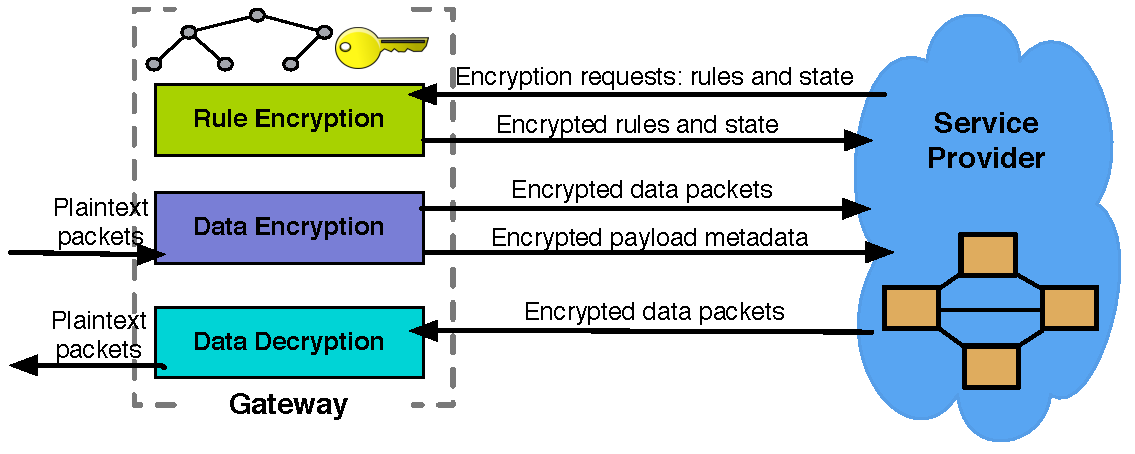
\includegraphics[width=3.25in]{fig/gateway2cloud}
  \caption[]{\label{fig:gatewaymeta} Communication between the cloud and gateway services: rule encryption, data encryption, and data decryption.} 
\end{figure}


%DIF > \eat{
%\begin{figure}[t]
%  \centering
%  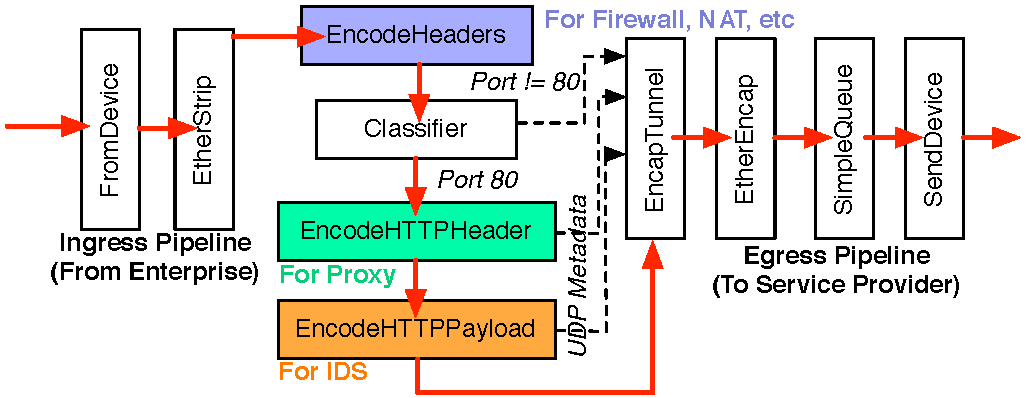
\includegraphics[width=3.25in]{fig/gatewaydiag}
%  \caption[]{\label{fig:gateway} Data encryption (enterprise to cloud) click module.}
%\end{figure}
%DIF > }




The gateway serves two purposes. First, it redirects traffic to/from the cloud for middlebox processing. Second, it provides the cloud with encryptions of rulesets and updates to the \DIFdelbegin \DIFdel{RangeMatch }\DIFdelend \DIFaddbegin \DIFadd{PrefixMatch }\DIFaddend tree.
Every gateway is configured statically to tunnel traffic to a fixed IP address at a single service provider point of presence.
A gateway can be logically thought of as three services: the rule encryption service, the pipeline from the enterprise to the cloud (Data encryption), and the pipeline from the cloud to the enterprise (Data decryption). 
All three services share access to the \DIFdelbegin \DIFdel{RangeMatch }\DIFdelend \DIFaddbegin \DIFadd{PrefixMatch }\DIFaddend tree and the private key $k$.
Figure~\ref{fig:gatewaymeta} illustrates  these three services and the data they send to and from the cloud provider.

We design the gateway with two goals in mind: 

\noindent{\bf Format-compatibility}: in converting plaintext traffic to encrypted traffic, the encrypted data should be structured in such a way that the traffic {\it appears as normal IPv6 traffic} to middleboxes performing the processing. Format-compatibility allows us to leave fast-path operations unmodified not only in middlebox software, but also in hardware components like NICs and switches; this results in good performance at the cloud.

\noindent{\bf Scalability and Low Complexity}: the gateway should perform only inexpensive per-packet operations and should be parallelizable. The gateway should not require configuration other than to generate a key and establish a session with the cloud provider. If the gateway were as expensive and complex as the middleboxes, there would be no cost or management benefits from outsourcing. 

%We now discuss how the gateway performs encryption and decryption (\S\ref{sec:dataenc}) and how rules are encrypted (\S\ref{sec:rulenc}) with these design goals in mind.

\subsection{Data Encryption and Decryption}
\label{sec:dataenc}

As shown in Table~\ref{tbl:mbreqs}, we categorize middleboxes as Header middleboxes, which operate only on IP and transport headers; \DIFdelbegin \DIFdel{HTTP middleboxes, which operate on HTTP headers and may operate on IP and transport headers; and }\DIFdelend \DIFaddbegin \DIFadd{and }\DIFaddend DPI middleboxes, which operate on arbitrary fields in a connection bytestream. We discuss how each category of data is encrypted/decrypted in order to meet middlebox requirements as follows.

\subsubsection{IP and Transport Headers}
IP and Transport Headers are encrypted field by field (\eg{}, a source address in an input packet results in an encrypted source address field in the output packet) with \DIFdelbegin \DIFdel{RangeMatch}\DIFdelend \DIFaddbegin \DIFadd{PrefixMatch}\DIFaddend .
We use \DIFdelbegin \DIFdel{RangeMatch }\DIFdelend \DIFaddbegin \DIFadd{PrefixMatch }\DIFaddend for these fields because many middleboxes perform analysis over prefixes and ranges of values -- e.g., a firewall may block all connections from a restricted IP prefix.

\noindent{\bf Decryption.} \DIFdelbegin \DIFdel{RangeMatch }\DIFdelend \DIFaddbegin \DIFadd{PrefixMatch }\DIFaddend is not reversible. To enable packet decryption, we store the \DIFdelbegin \DIFdel{AES encrypted }\DIFdelend \DIFaddbegin \DIFadd{AES-encrypted }\DIFaddend values for the header fields in the \DIFdelbegin \DIFdel{IP }\DIFdelend \DIFaddbegin \DIFadd{IPv6 }\DIFaddend options header. When the gateway receives a packet to decrypt, it decrypts the values from the options header and restores them.% to the IP or transport header.

\noindent{\bf Format-compatibility.} 
Our modifications to the IP and transport headers place the encrypted \DIFdelbegin \DIFdel{range }\DIFdelend \DIFaddbegin \DIFadd{prefix }\DIFaddend match data back in to the same fields as the unencrypted data was originally stored; because comparisons between rules and encrypted data rely on $\leq$ $\geq$, just as unencrypted data, this means that operations performing comparisons on IP and transport headers {\it remain entirely unchanged at the middlebox.}
This ensures backwards-compatibility with existing software {\it and hardware} fast-path operations.
Because per-packet operations are tightly optimized in production middleboxes, this compatibility ensures good performance at the cloud despite our changes.

An additional challenge for format compatibility is where to place the decryptable AES data; one option would be to define our own packet format, but this could potentially lead to incompatibilities with existing implementations. By placing it in the IPv6 options header, middleboxes can be configured to ignore this data.\footnote{It is a common misconception that middleboxes are incompatible with IP options. Commercial middleboxes are usually aware of IP options but many administrators {\it configure} the devices to filter or drop packets with certain kinds of options enabled.}


\subsubsection{Payload Data} 
The connection bytestream is encrypted with KeywordMatch.
This allows \sys to support DPI middleboxes, such as intrusion detection or exfiltration prevention.
These devices must detect whether or not there exists an exact match for an encrypted rule string {\it anywhere} in the connection bytestream.
Because this encrypted payload data is over the {\it bytestream}, we need to generate encrypted values which span `between' packet payloads. 
Searchable Encryption schemes, which we use for encrypted DPI, require that traffic be {\it tokenized} and that a set of fixed length substrings of traffic be encrypted along a sliding window -- e.g., the word malicious might be tokenized into {'malici', 'alicio', 'liciou', 'icious'}.
If the term 'malicious' is divided across two packets, we may not be able to tokenize it properly unless we reconstruct the TCP bytestream at the gateway. Hence, if DPI is enabled at the cloud, we do exactly this.

\DIFdelbegin \DIFdel{The }\DIFdelend \DIFaddbegin \DIFadd{After reconstructing and encrypting the TCP bytestream, the }\DIFaddend gateway transmits the encrypted bytestream over an `extension', secondary channel that only those middleboxes which perform DPI operations inspect. This channel is not routed to other middleboxes. \DIFaddbegin \DIFadd{We implement this channel as a persistent TCP connection between the gateway and middleboxes. The bytestream in transmission is associated with its flow identifier, so that the DPI middleboxes can distinguish between bytestreams in different flows.
}\DIFaddend 

\DIFaddbegin \DIFadd{Besides, the gateway still forward the packets to the cloud, with the payload data encrypted with AES and checksums recomputed. The DPI middleboxes handle the packets based on the bytestream received from the extension channel.
}

\DIFaddend \noindent{\bf Decryption.} The payload data is encrypted with AES and placed back into the packet payload -- like \DIFdelbegin \DIFdel{RangeMatch}\DIFdelend \DIFaddbegin \DIFadd{PrefixMatch}\DIFaddend , KeywordMatch is not reversible and we require this data for decryption at the gateway.
Because the extension channel is not necessary for decryption, it is not transmitted back to the gateway.

\noindent{\bf Format-compatibility.} To middleboxes which only inspect/modify packet headers, encrypting payloads has no impact. 
By placing \DIFdelbegin \DIFdel{this data }\DIFdelend \DIFaddbegin \DIFadd{the encrypted bytestreams }\DIFaddend in the extension channel, the extra traffic can be routed past and ignored by middleboxes which do not need this data. % hence it will not interfere with normal processing. 

DPI middleboxes which do inspect payloads must be modified to inspect the extension channel alongside the primary channel, as described in~\cite{blindbox}; DPI devices are typically implemented in software and and these modifications are both straightforward and introduce limited overhead (as we will see in \S\ref{sec:eval}). 

\subsubsection{HTTP Headers} 

HTTP Headers are a special case of payload data. Middleboxes such as web proxies do not read arbitrary values from packet payloads: the only values they read are the HTTP headers. \DIFdelbegin \DIFdel{We }\DIFdelend \DIFaddbegin \DIFadd{They can be categorized as DPI middleboxes since they need to examine the TCP bytesteam. However, due to the limitation of full DPI support, we }\DIFaddend treat these values specially compared to other payload data: we encrypt the entire (untokenized) HTTP URI using a deterministic form of KeywordMatch.

Normal KeywordMatch permits comparison between encrypted values and rules, but not between one value and another value; deterministic KeywordMatch permits two values to be compared as well.
Although this is a weaker security guarantee relative to KeywordMatch, it is necessary to support web caching which requires comparisons between different URIs.
The cache hence learns the frequency of different URIs, but cannot immediately learn the URI values.
 This is the only field which we encrypt in the weaker setting.
We place this encrypted value in the extension channel; hence our HTTP encryption has the same format-compatibility properties as other DPI devices.

Like other DPI tasks, this requires parsing the entire TCP bytestream. However, in some circumstances we can extract and store the HTTP headers statelessly; so long as HTTP pipelining is disabled and packet MTUs are standard-sized (>1KB), the required fields will always appear contiguously within a single packet. \DIFaddbegin \DIFadd{Given that SPDY uses persistent connections and pipelined requests, this stateless approach does not apply to SPDY.
}\DIFaddend %Hence, if DPI is disabled we can avoid reconstructing the TCP bytestream at the middlebox.
%When DPI is enabled, the gateway scans through every byte of data in the connection already;  extracting these headers allows the middlebox to avoid re-doing work which has already been done at the gateway.

\noindent{\bf Decryption.} The packet is decrypted as normal using the data stored in the payload; \DIFaddbegin \DIFadd{IP }\DIFaddend options are removed.


%DIF > \eat{
%JS: I vote to cut this. Here's why -- we are going to be basically hosed when it comes to bandwidth, whether or not we have this. And adding this in adds a huge amount of complexity to the gateway! So way sacrifice our primary goal (cheap, less complex) to only partially fix another problem??
%\subsubsection{Optimizing Decryption}
%DIF < To reduce bandwidth usage, the gateway temporarily caches the packets destined to the service provider indexed by their hashes for a short time. If the middleboxes on the cloud do not change the packet content, instead of sending the whole packet back, the service provider sends a control packet %containing the hash of the original packet. The gateway then retrieves the local packet by looking up the hash in the cache.
%DIF > To reduce bandwidth usage, the gateway temporarily caches the packets destined to the service provider indexed by their hashes for a short time. If the middleboxes on the cloud do not change the packet content, instead of sending the whole packet back, the service provider sends a control packet containing the hash of the original packet. The gateway then retrieves the local packet by looking up the hash in the cache.
%DIF > }

\subsection{Rule Encryption}
\label{sec:rulenc}

Rules for firewalls and DPI services come from a variety of sources and can have different policies regarding who is or isn't allowed to know the rules. 
For example, exfiltration detection rules may include keywords for company products or unreleased projects which the client may wish to keep secret from the cloud provider. 
On the other hand, many DPI rules are proprietary features of DPI vendors, who may allow the provider to learn the rules, but not the client.
\sys supports three different models for KeywordMatch rules which allow clients and providers to share rules as they are comfortable: (a) the client knows the rules, and the provider does not; (b) the provider knows the rule, and the client does not; or (c) both parties know the rules.
\DIFdelbegin \DIFdel{RangeMatch }\DIFdelend \DIFaddbegin \DIFadd{PrefixMatch }\DIFaddend rules only supports (a) and (c) -- the gateway who maintains the rule tree {\it must} know the rules to perform encryption properly.

If the client is permitted to know the rules, they encrypt them -- either generating a KeywordMatch, AES, or \DIFdelbegin \DIFdel{RangeMatch }\DIFdelend \DIFaddbegin \DIFadd{PrefixMatch }\DIFaddend rule -- and send them to the cloud provider. If the cloud provider is permitted to know the rules as well, the client will send these annotated with the plaintext for each encryption; if the cloud provider is not allowed, the client sends only the encrypted rules in random order.

If the client is not permitted to know the rules, we must somehow allow the cloud provider to learn the encryption of each rule with the client's key. This is achieved using a classical combination of Yao's garbled circuits~\cite{Yao86} with oblivious transfer~\cite{Naor-Pinkas}, as originally applied by BlindBox~\cite{blindbox}.
As in BlindBox, this exchange only succeeds if the rules are signed by a trusted third party (such as McAffee, Symantec, or EmergingThreats) -- the cloud provider should not be able to generate their own rules without such a signature as it would allow the cloud provider to read arbitrary data from the clients' traffic.
Unlike BlindBox, this rule exchange occurs exactly once -- when the gateway initializes the rule. 
After this setup, all connections from the enterprise are encrypted with the same key at the gateway.
%This is important because for a typical industry ruleset, a garbled circuit + oblivious transfer exchange takes 97 seconds~\cite{blindbox}; with BlindBox this exchange must be performed for every connection and thus is prohibitive for practicality.
%For \sys, on the otherhand, this amounts to a relatively cheap one-time setup cost.

%DIF > \eat{
%\subsection{Discussion}
%\label{sec:gwimpl}
%DIF < We built our gateway as described above using Click over DPDK on an off-the-shelf 16-core server with 2.6GHz Xeon E5-2650 cores and 128GB RAM; the network hardware is a single 10GbE Intel 82599 compatible network card. 
%DIF > We built our gateway as described above using BESS~\cite{bess} on an off-the-shelf 16-core server with 2.6GHz Xeon E5-2650 cores and 128GB RAM; the network hardware is a single 10GbE Intel 82599 compatible network card. 
%We discuss a few systems properties of our gateway as follows before discussing middlebox implementations in \S\ref{sec:mbimpl}.
%
%DIF > \eat{
%Our gateway datapath implementation has 3 major components: Header Rewrite, Stream Reconstruction, and Packet Cache. We primarily introduce the dataflow from the client to the gateway below:
%
%DIF < \noindent\textbf{Header Rewrite.} At this stage, the gateway rewrites the header fields in the packets using the RangeMatch scheme using in algorithm in Section \ref{sec:dataenc}. It consists of multiple Click elements: ProtocolTranslator46 that translates an IPv4 packet to an IPv6 packet, AppendIP6Option that populates DET-encrypted header fields into the IPv6 options, HeaderEncrypt that performs the encryption, and SetTCPChecksum that sets the checksum.
%DIF > \noindent\textbf{Header Rewrite.} At this stage, the gateway rewrites the header fields in the packets using the PrefixMatch scheme using in algorithm in Section \ref{sec:dataenc}. It consists of multiple Click elements: ProtocolTranslator46 that translates an IPv4 packet to an IPv6 packet, AppendIP6Option that populates DET-encrypted header fields into the IPv6 options, HeaderEncrypt that performs the encryption, and SetTCPChecksum that sets the checksum.
%
%\noindent\textbf{Stream Reconstruction.} This component acts as a TCP transparent proxy by terminating incoming TCP connections from clients. It encrypts the reconstructed bytestreams using the stream cipher, and relays them in new connections. Note that the IP options are preserved during this phase. It also pushes bytestreams into the secondary channel, where middleboxes can perform DPI operations. Meanwhile, it extracts HTTP headers from the stream and puts the deterministically encrypted HTTP header fields into the IP options.
%
%\noindent\textbf{Packet Cache.} The dataflow from the service provider back to the gateway is relatively simple. The Packet Cache restores the packets, the Stream Reconstruction component decrypts the streams into plaintext, then the Header Rewrite component decrypts the header fields and performs 6to4 translation (if the client uses IPv4).
%
%Having discussed the design and implementation of the gateway, we now revisit a few of its system properties before moving on to the design and implementation of the middleboxes in \S\ref{sec:mbimpl}.
%DIF > }
%
%\noindent\textbf{Scalability.}
%Encryption and decryption are entirely parallel: they require no synchronization or communication between threads. We show in \S\ref{sec:eval} that we achieve almost linear improvements from adding additional processing cores.
%However, per-packet operations rely only on relatively inexpensive techniques; the most expensive operation performed is AES encryption with is supported in hardware through the AES-NI instructions. 
%Consequently, the gateway can support 10Gbps of traffic with only 8 cores enabled.
%
%\noindent\textbf{Complexity.}
%An administrator only supplies the gateway with the IP address of the cloud and the secret key $k$.
%The administrator places the gateway at the border of their enterprise network to the Internet.
%The administrator supplies any rules/policies to the cloud provider and the gateway is then configured by the cloud provider.
%
%\noindent\textbf{Fault Tolerance.}
%DIF < When DPI is disabled, the gateway keeps no per-connection state. Hence, a cold standby can take over correctly for the gateway so long as it has the `static' state of the RangeMatch tree, key $k$, and IP address of SP.
%DIF > When DPI is disabled, the gateway keeps no per-connection state. Hence, a cold standby can take over correctly for the gateway so long as it has the `static' state of the PrefixMatch tree, key $k$, and IP address of SP.
%When DPI is enabled, the gateway maintains the last few packets from each connection (window-length) to perform tokenization; under these conditions the gateway can use standard techniques for backup including an active standby~\cite{colo}.
%DIF > }

%DIF > !TEX root = mb.tex
\DIFaddbegin 


\DIFaddend \section{Middleboxes: Design \& Implementation}
\label{sec:mbs}

In Table~\ref{tbl:mbreqs}, we introduced the set of middleboxes typically supported by outsourcing approaches\DIFdelbegin \DIFdel{and divided them in to Header, HTTP, and DPI middleboxes}\DIFdelend . We now revisit these middleboxes individually. %and discuss how they operate over the encrypted data.

\subsection{Header Middleboxes}
Middleboxes which operate on IP and transport headers only include firewalls, NATs, and \DIFaddbegin \DIFadd{L3/}\DIFaddend L4 load balancers.
Firewalls are read-only, but NATs and L4 load balancers may rewrite IP addresses or port values. 
For header middleboxes, per-packet operations remain unchanged for both read and write operations.

For read operations, the firewall receives a set of encrypted rules from the gateway and compares them directly against the encrypted packets just as normal traffic. Because \DIFdelbegin \DIFdel{RangeMatch }\DIFdelend \DIFaddbegin \DIFadd{PrefixMatch }\DIFaddend supports $\leq$ and $\geq$, the firewall may use any of the standard classification algorithms~\cite{packet_classif}.

For write operations, the middleboxes assign values from an address pool; it receives these encrypted pool values from the gateway during the rule generation phase.
These encrypted rules are marked with a special suffix reserved for rewritten values.
When the gateway receives a packet with such a rewritten value, it restores the plaintext value from the pool rather than decrypting the value from the options header.

\DIFaddbegin \DIFadd{Middleboxes can recompute checksums as usual after they write.
}

\DIFaddend \subsection{DPI Middleboxes}
We modify middleboxes which perform DPI operations as described by BlindBox~\cite{blindbox}. 
The middleboxes search through the encrypted extension channel -- not the packet payloads themselves -- and block \DIFaddbegin \DIFadd{or log }\DIFaddend the connection if a blacklisted term is observed in the extension.
Much of the BlindBox paper is devoted to designing new fast-path algorithms which provide high throughput and cryptographic compatibility; as we showed \sys sidesteps this problem for header middleboxes since it can re-use existing algorithms.

\subsection{HTTP Middleboxes}
Parental filters and \DIFdelbegin \DIFdel{L7 Load Balancers }\DIFdelend \DIFaddbegin \DIFadd{HTTP proxies }\DIFaddend read the HTTP URI from the \DIFdelbegin \DIFdel{options header}\DIFdelend \DIFaddbegin \DIFadd{extension channel}\DIFaddend . 
If the parental filter observes a blacklisted URI, it drops \DIFaddbegin \DIFadd{packets that belong to }\DIFaddend the connection.
\DIFdelbegin \DIFdel{The L7 load balancer uses the URI to rewrite the IP header, and operates exactly like a NAT or L4 LB, except that it uses the URI to select which destination address to assign new connections.
}\DIFdelend %DIF > The L7 load balancer uses the URI to rewrite the IP header, and operates exactly like a NAT or L4 LB, except that it uses the URI to select which destination address to assign new connections.

The web proxy required the most modification of any middlebox \sys supports; nonetheless, our proxy achieves good performance as we will discuss in \S\ref{sec:eval}.
The proxy caches HTTP static content (e.g., images) in order to improve client-side performance. 
When a client opens a new HTTP connection, a typical proxy will capture the client's SYN packet and open a new connection to the client, as if the proxy were the web server. The proxy then opens a second connection in the background to the original web server, as if it were the client. 
When a client sends a request for new content, if the content is in the proxy's cache, the proxy will serve it from there. Otherwise, the proxy will forward this request to the web server and cache the new content. 

The proxy has a map of encrypted file path to encrypted file content. When the proxy \DIFdelbegin \DIFdel{receives a packet}\DIFdelend \DIFaddbegin \DIFadd{accepts a new TCP connection on port 80}\DIFaddend , the proxy extracts the encrypted URI \DIFdelbegin \DIFdel{from the options header }\DIFdelend \DIFaddbegin \DIFadd{for that connection from the extension channel }\DIFaddend and looks it up in the cache. The use of deterministic encryption enables the proxy to use a fast search data structure/index, such as a hash map, unchanged. We have two \DIFaddbegin \DIFadd{possible }\DIFaddend cases: there is a hit or a miss. \DIFdelbegin \DIFdel{For }\DIFdelend \DIFaddbegin \DIFadd{If there is a cache }\DIFaddend hit, the proxy \DIFdelbegin \DIFdel{assembles a packet header for reverse traffic and attaches to it }\DIFdelend \DIFaddbegin \DIFadd{sends }\DIFaddend the encrypted file content from the cache \DIFaddbegin \DIFadd{via the existing TCP connection}\DIFaddend . Even without being able to \DIFdelbegin \DIFdel{encrypt }\DIFdelend \DIFaddbegin \DIFadd{decrypt }\DIFaddend IP addresses or ports, the proxy can \DIFdelbegin \DIFdel{create the header by reversing the encrypted information in the original header .
For a }\DIFdelend \DIFaddbegin \DIFadd{still accept the connection, as the gateway encrypts/decrypts the header fields transparently.
If there is a cache }\DIFaddend miss, the proxy \DIFdelbegin \DIFdel{forwards the }\DIFdelend \DIFaddbegin \DIFadd{opens a new connection and forwards the encrypted }\DIFaddend request to the web server\DIFdelbegin \DIFdel{, once again copying the IP address, ports, and options. When receiving the response , the proxy caches it to serve future requests. }\DIFdelend \DIFaddbegin \DIFadd{. Recall that the traffic bounces back to gateway before being forwarded to the web server, so that the gateway can decrypt the header fields and payloads. Conversely, the response packets from the web server are encrypted by the gateway and received by the proxy. The proxy then caches and sends the encrypted content back. The content is separated by packets. Packet payloads are encrypted on a per-packet basis. Hence, the gateway can decrypt them correctly.
}\DIFaddend 




%DIF < input{headerMB}
%DIF < %!TEX root = mb.tex



\section{Middlebox: IDS and exfiltration detection}\label{sec:ids}

In intrusion detection or prevention~\cite{Snort}, a middlebox (IDS or IPS) attempts to detect intrusion attacks by looking to match attack signatures against the traffic.
In data exfiltration prevention~\cite{CMU_exfiltration_report}, a middlebox attempts to detect if a malicious employee of an organization 
attempts to exfiltrate confidential data, as follows.  The confidential data has watermarks in it, the middlebox knows these watermarks and tries to find them
in the traffic. 

Unlike the previously presented middleboxes, these middleboxes are bytestream aware:  they operate over the TCP bytestream, as opposed to over each packet individually. Hence, deploying an IDS at the cloud requires a stateful gateway at the enterprise.

\sys's IDS builds on top of BlindBox~\cite{blindbox}, an IDS which uses searchable encryption to detect malicious signatures within encrypted HTTPS connections. We now  summarize, but exclude many important details all of which are presented in~\cite{blindbox}.

\mypara{BlindBox}
To encrypt a stream of traffic from a sender, BlindBox first generates tokens from the stream.  
For simplicity, consider that BlindBox generates a token for  every byte offset in the unencrypted payload (for a more efficient technique, see~\cite{blindbox}). 
The  token encodes the first N = 8 bytes starting at the byte offset. Then, it encrypts the tokens with KeywordMatch, which we discussed in \S\ref{s:kwmatch}.
For example, a sender transmitting the word `malicious' would transmit the encrypted tokens for [$\enc$(`maliciou'), $\enc$(`alicious')].

 {\em Model 1.} BlindBox adds these encrypted tokens to the  regular HTTPS traffic, on  a secondary channel.
An IDS looking for the word `malicious' would declare a match if it observes both these tokens consecutively.
For data exfiltration detection and for IDS signatures which consist {\it only} of exact match signatures, KeywordMatch is sufficient to detect attacks.
The security guarantee it gives is as in KeywordMatch (\S\ref{s:kwmatch}): for every suspicious $N$-byte string part of the suspicious signatures at the IDS, the IDS learns if the string matches at a certain offset in the packet, but it does not learn anything else. In particular, if the stream contains no suspicious strings, the middlebox learns virtually nothing about the stream. 

 {\em Model 2.}  While this covers the case of data exfiltration and a significant number of IDS signatures, it does not support  IDS signatures with regular expressions.
 In fact, there exists no encryption scheme that can support such generic computation over encrypted data in a practical way in the literature. 
  Hence, to support regular expressions, BlindBox -- and hence \sys -- provide a secondary protocol with a different security guarantee. 
  Based on Snort's manual~\cite{Snort_manual}, all  IDS signatures must include exact match strings that filter a lot of the traffic -- for performance reasons, an IDS like Snort~\cite{Snort} performs regular expression detection after all exact match strings have been matched first.
  Inspired by this, BlindBox allows the middlebox to decrypt all the packets in the session if and {\it only} if a suspicious exact match strings matches a packet in this session.
  Namely, if there is a reason to suspect the session is malicious, the middlebox will be able to decrypt it and see its contents, but if there is no suspicious content, the middlebox cannot physically decrypt the traffic.  This model is called `probable cause decryption'.
  The client encodes the key with the tokens such that if a match occurs, the middlebox can automatically decrypt the key (once again, details are in~\cite{blindbox}).
  Now, if there is a match and the packet gets decrypted, the middlebox can run the regular expressions on the unencrypted traffic as before. 
  
  
  In summary, the first model is more secure but less expressive: 
  the first model allows the middlebox to {\it detect a substring}, only if that substring is suspicious;
  the second model allows the middlebox to {\it decrypt the entire stream} if a substring is suspicious.
  
\mypara{\sys's IDS}  
  Everything we have described so far is identical between BlindBox and \sys. We now describe how they are different, and how \sys improves performance and security.

The key difference between BlindBox and \sys's IDS comes from the cost to setup signatures at the IDS. 
With \sys, the gateway can simply encrypt rules with its key $k$ and transmit them to the IDS, who then applies them over the enterprise's traffic.
With BlindBox, this is not appropriate.
BlindBox aims to allow a client (\eg{} laptop) connecting to {\em any} receiver to receive IDS processing over their HTTP traffic, even if the IDS is unknown or untrusted to them.
Hence, the middlebox cannot give the signatures to the client both to prevent the client from avoiding detection~\cite{Bro} and to prevent the client from leaking these expensive signatures. 
In this scenario, the IDS wants to {\it enforce} that all traffic be scanned for malicious behavior, but the client wants to maintain {\it privacy} from the untrusted IDS.
As a result, the middlebox will not give its rules to the client, and the client will not give its key to the middlebox.
Hence,  to generate the encrypted rules that the IDS can use for detection requires BlindBox to perform
a sophisticated cryptographic computation (based on a primitive called garbled circuits~\cite{Yao82}) at the start of each connection, which makes the connection
startup time slow. 
Further, this computation scales with the number of exact-match rules the IDS needs to learn: the more rules, the longer the startup time.
%\sys does not have such overhead.

Fortunately, the setup in \sys is different: even though the client is untrusted, the gateway is trusted. Hence, the middlebox can give the signatures to the gateway which can encrypt them using simple AES. Moreover, the gateway can perform this encryption once and does not need to repeat it for every user session. 
There are two implications of this: better performance and better security.

\textit{Better performance.}
The first implication is performance: this startup time is eliminated, as the signatures are generated once, at the gateway, and transmitted to the IDS. After this there is no more setup cost. This improves the overall time to setup a connection by orders of magnitude, as discussed in \S\ref{sec:eval}. 

\textit{Better security.}
The second implication is improved security. We made the observation that, since setting up a signature is cheaper, we can generate more signatures and hopefully reduce some regular expression signatures to a set of exact matches.  
For example, the regular expression 'alice[1-3]' is equivalent to any of the exact matches [`alice1', `alice2', `alice3']. 
Not all rules are amenable to this -- \eg{} `bob[a-z]+' would result in a prohibitively large (and also far too general) number of expansions, even for \sys. 
Hence, we try to expand each regular expression that has a modest expansion into exact match signatures. 
%To do this expansion with BlindBox would be prohibitively expensive, as each additional exact match rules increases the already lengthy setup time.
%However, as \sys has no such cost, we can expand many regular expressions and thus detect them using the stronger security model.
For the signatures that we could expand, \sys provides the security of Model 1 whereas BlindBox provides Model 2, and hence \sys improves security. 
The more signatures we can support this way, the less often the middlebox is able to perform stream decryption. 
In \S\ref{sec:eval}, we evaluate existing signature sets, and find that regular expression expansion almost doubles the number of signatures that can be detected using the stronger security model.


%Like proxies, Intrusion Detection/Prevention systems operate over packet payloads, not just the IP/TCP/UDP headers.
%IDS/IPS are canonical examples of DPI devices.



%DIF < %!TEX root = mb.tex

\section{Other middleboxes}\label{sec:vpn} \label{sec:other_apps} \label{sec:not_supp}\label{sec:loadb}

In this section, we discuss briefly other middleboxes \sys supports, which are straightforward extensions of the ones presented so far. 

\bpara{L4 and L7 Load balancer} 
The L4 load balancer spreads the load from packets destined to the same IP address across different servers. \sys supports this middlebox in a 
very similar way to the NAT presented in \S\ref{sec:nat}. The L7 load balancer spreads the load destined for the same URL or path across 
different servers. \sys supports this middlebox in a very similar way to the web proxy presented in \S\ref{s:proxy}. 


\bpara{IP forwarding} This middlebox is implemented similarly to a NAT and firewall. 


\bpara{VPN} The APLOMB~\cite{aplomb} model supports the VPN by installing an APLOMB client at the user endpoint, as part of the VPN client.
\sys also installs a \sys client as part of the VPN client which does the encryption and decryption work of the gateway. The VPN middlebox remains
largely the same because it does not compute on the traffic. 


\bpara{Application firewall} This middlebox is a simple version of an IDS combined with a firewall. 


\bpara{WAN optimizers} WAN optimizers compress network traffic. APLOMB~\cite{aplomb} requires the compression to happen
at the gateway, because otherwise, it loses the bandwidth benefits of the compression. Hence, this middlebox does not benefit much 
 from the cloud outsourcing. 
Nevertheless, we can still support it. 
If the other middleboxes used are only header middleboxes, WAN optimizers can be  supported without modification.
If one uses an IDS middlebox too, \sys  requires  the IDS tokenization  to run before the compression so it can tokenize
the traffic; in this case, unfortunately, \sys  reduces the compression benefit of the WAN optimizer because the encrypted tokens 
are not compressible. 




% some potentially useful things
%\section{Discussion}
%
%No one will put a firewall behind a NAT
%
%since we are giving primitives, one might be able to add later applications that can also be supported with the same primitives, although one has to add encryption at the gateway for the specific fields 
%
%What do we do about these issues?
%
%Checksum Many middleboxes change packet contents, and thus packet check-
%sums. However, it is not clear that if we can compute correct checksums based
%
%on encrypted packet contents.
%
%IP Fragmentation Middleboxes working above L3 may need to reassemble
%
%IP fragments, our encryption scheme need to be carefully designed to avoid any
%
%issues.



%DIF < %!TEX root = mb.tex

\section{System implementation} \label{sec:impl}
\eat{
\todo{this is important to write properly because it is a systems paper and there were some nontrivial decisions}.

Things to cover:

- gateway and middlebox implementation

- explain why the firewall hardware does not change (or was that above?)

- second flow udp/tcp

- might want to explain these points made in intro: "
Sylvia, it would be great if you could read and revise the paper. Feel free to edit directly in tex!
We really need your feedback at this stage."

- new packet structure and headers -- multiple layers of headers? graph? (there is some text and a figure in a google doc about this)

- some things are specific to web proxy from what I remember
}

We now describe the \sys architecture and implementation. 
As discussed in \S\ref{sec:overview}, \sys redirects traffic to the cloud and back for {\it middlebox processing} using a {\it redirection gateway}.
%\todo{Put a little overview aout gateway, metadata channel, mbs here???}
We now present the implementation and architecture of the redirection gateway (\S\ref{sec:gateway}), followed by the modifications we made to middleboxes to support \sys (\S\ref{sec:middleboxes}).
%Finally, we discuss our EC2 deployment of these components (\S\ref{sec:deployment}).


\subsection{Redirection \& gateway implementation}
\label{sec:gateway}

\begin{figure}[t]
  \centering
  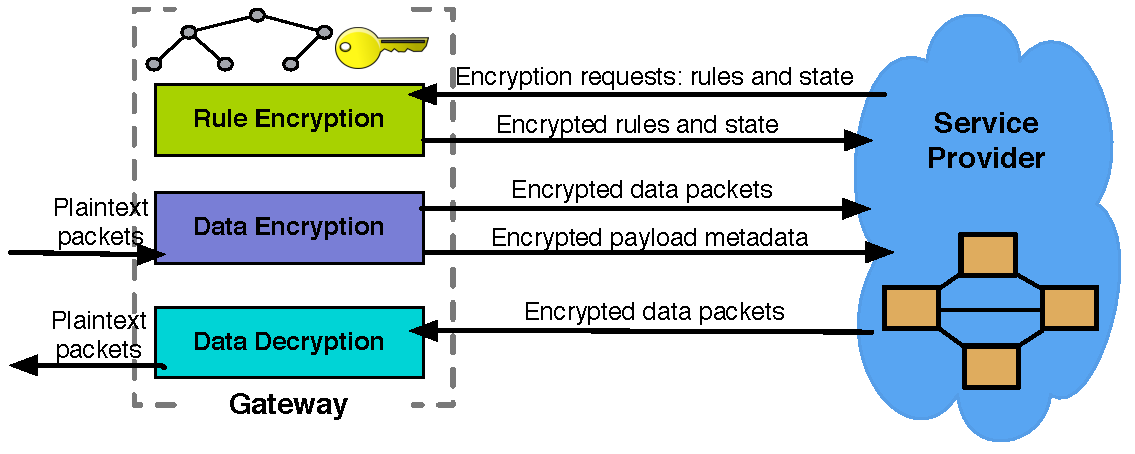
\includegraphics[width=3.25in]{fig/gateway2cloud}
  \caption[]{\label{fig:gatewaymeta} Communication between the cloud and gateway services: rule encryption, data encryption, and data decryption}
\end{figure}



\begin{figure}[t]
  \centering
  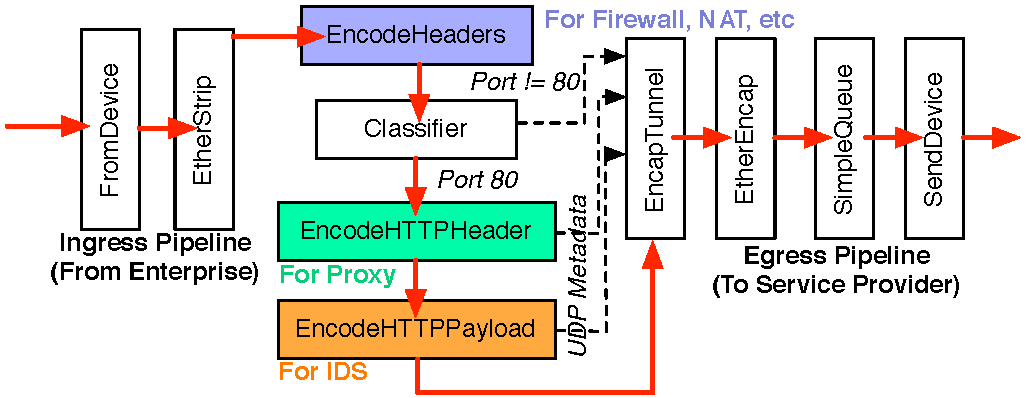
\includegraphics[width=3.25in]{fig/gatewaydiag}
  \caption[]{\label{fig:gateway} Data encryption (enterprise to cloud) click module.}
\end{figure}

The gateway serves two purposes. First, it redirects traffic to/from the cloud for middlebox processing. Second, it provides the cloud with encryptions of IDS/FW rulesets and updates to the RangeMatch tree.
Every gateway is configured statically to tunnel traffic to a fixed IP address at a single service provider point of presence.
A gateway can be logically thought of as three services: the rule encryption service, the pipeline from the enterprise to the cloud (Data encryption), and the pipeline from the cloud to the enterprise (Data decryption). 
All three services share access to the RangeMatch tree and the private key $k$.
Figure~\ref{fig:gatewaymeta} illustrates  these three services and the data they send to and from the cloud provider.

\noindent{\bf Rule Encryption.} The rule encryption component provides the cloud provider with encrypted rules/policies to use at the middlebox. 
There are two possible ways rules can be generated. First, an enterprise may choose to generate their own rules, in which case, they send encrypted versions of the rules directly to the cloud.
Rules can contain IP addresses, port numbers, and substrings of attack signatures; the first two must be encrypted with both keyword match and range match, the last needs only to be encrypted with keyword match.
Alternately, the enterprise may opt in to a `default' set of rules from the cloud provider, in which case the cloud provider sends the rules to the gateway which encrypts them and sends them back.
The rule encryption component also sends rule updates. Whenever an adjustment is made to the RangeMatch table, it sends an update to the cloud provider with the adjusted mappings/rules.
If the gateway ever changes its key, the encryption component must also signal to the cloud provider and re-encrypt all rules.
%\todo{too high level? Details about how updates work?}

\noindent{\bf Data Encryption.} In Figure~\ref{fig:gateway}, we show the DPDK-Click~\cite{click} packet processing pipeline that implements data encryption and transmits packets from the enterprise to the cloud.
Traffic that is returning from the Internet and traffic that is about to be sent to the Internet are both sent along this pipeline.
This figure assumes the enterprise is already using IPv6, if it is not, the pipeline would also include a `4to6' element.
In \S\ref{sec:overview}, we described how \sys encodes packet content using the AES, Keyword Match, and Range Match encryption algorithms. 
The encrypted values are placed either directly back in to a data packet, or transmitted over a {\it metadata channel}.

Below, we detail the three elements we implemented to encrypt the packet data:

\noindent {\it Encode Headers:} Encrypts the IP, TCP, and UDP headers, replacing all IP and Port numbers in the packet with values calculated using the {\it RangeMatch} encryption algorithm. Appends the AES-encrypted values to the IP options field of the data packet.
Required to support all middleboxes. 

\noindent {\it Encode HTTP Header.} Encrypts the HTTP header for {\it the first GET request only.} Does not modify the data packet itself, but instead places the keyword match encryptions of the values in a new packet sent over the metadata channel. \clan{Here! And we also mention this in Section 8.2}
The new packet marks (a) the encrypted 5-tuple flow ID for the packet, (b) that this is HTTP GET data for the proxy, and (c) the encrypted values. At the cloud, the proxy can read this metadata channel to obtain the encrypted URL for the GET request and check its cache for the encrypted data. This element is only needed if there is an HTTP proxy enabled at the cloud, otherwise it can be disabled at the gateway.

\noindent {\it Encode HTTP Payload.} Encrypts the entire HTTP payload (as described in \S\ref{sec:ids}), placing the keyword match values in a new packet in the metadata channel. Unlike the other two elements, this element keeps per-flow state, reconstructing the TCP stream in order to generate keyword match tokens for keywords which are divided across two subsequent packets.  The metadata channel packets contain (a) the encrypted 5-tuple for the packet, (b) that the packet contains keyword match data for the IDS, and (c) the encrypted values. At the cloud, the IDS can read this metadata channel to detect attacks; if there is a match it instructs the firewall to block the 5-tuple for the flow. This element is only needed if there is an IDS enabled at the cloud, otherwise it can be disabled at the gateway.


\noindent{\bf Data Decryption.} Packets returning from the cloud follow a much simpler packet processing pipeline than those being encrypted.
The packet payloads are decrypted using standard AES; the IP and port values from the options header are decrypted and then copied in to the packet header. The options header is removed.
If the enterprise is running IPv4, the traffic is sent back through the 4to6 converter to convert the packet back to IPv4.
The packet is then sent out to the Internet or the client at the enterprise.


\subsection{Middlebox implementations}
\label{sec:middleboxes}

\begin{figure}[t]
  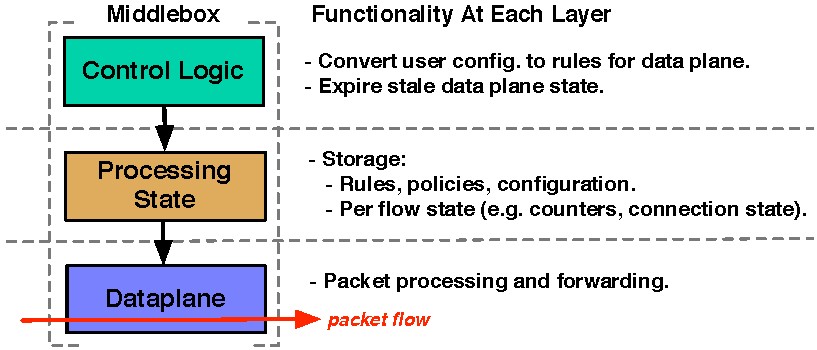
\includegraphics[width=3.25in]{fig/mbarch}
  \caption[]{\label{fig:mbarch} Typical middlebox software components. For most middleboxes, packet processing operations in the dataplane remain unmodified by \sys.}
\end{figure}

We implemented \sys for all middleboxes listed in Table~\ref{tab:apps-ops} using DPDK-Click~\cite{click}, with varying levels of modification to a baseline (unencrypted) design required to make them compatible with \sys. 
Figure~\ref{fig:mbarch} guides our discussion of these changes. %Most middlebox codebases can be divided in to three categories of functionality.
Although  middlebox software architectures are unlikely to be cleanly divided in to three independent components as shown, most classes and functions within a middlebox codebase can be labeled as one of these three categories.
These categories are: the dataplane (which performs packet processing), the middlebox state (which stores and updates rules and policies, as well as per-flow state like counters and connection state), and the control logic (which converts user configurations to rules and policies, and updates/refreshes state). 
Importantly, packet processing only occurs in dataplane functions, which are usually tightly engineered to process each packet in microseconds or faster.

We adapted all header-only middleboxes {\it without modifying steady-state dataplane functions}, and hence preserving the performance properties of the existing middleboxes.
We were able to do this because the encrypted values in the IPv6 header are stored in the normal IPv6 header formats, and because our encryption schemes preserve the exact match and range match semantics these devices use to operate correctly.
All we need to do to be compatible with normal dataplane behavior is to encrypt all values in the rules and configuration files using the the range match encryption algorithm.

We do need to change the control logic and add one `special case' check to the dataplane; this is to handle rule {\it updates}. 
The update code is triggered rarely -- when the gateway changes its key $k$, or when there is an update to the Range Match tree.
In this case the rules must be re-encrypted, and any per-session state (\eg{} the flow table in the NAT) must be re-encrypted as well.
When such an update is about to occur, the gateway first re-computes all rules {\it before} it begins to use the new encryption values on traffic. It signals to the cloud provider that it is about to perform a rule update. Then, all middleboxes transmit their rules / state tables to the gateway for re-encryption. 
Once all middleboxes have received their updated rules and state, the gateway `switches' to the new ruleset, sending a signal packet in the dataplane. When a middlebox receives this signal packet (the only change we make to the dataplane is to check for this signal packet) it switches out the ruleset to use the new values.~\footnote{\small There is a race condition for the flow state: consider a SYN packet which arrives just before the signal packet at a NAT. The NAT will encode the SYN packet in its state table using the old encryption scheme, and then immediately need to switch over to the new encryption scheme -- before it has the new mapping for the new flow. The middlebox will then immediately request a new encryption for the rule. Hence, a small number of packets may be misclassified during the transition.}
\todo{This is ugly as sin! Sigh! Can we do better?}  

Bytestream-aware middleboxes require changes in the dataplane as well as the control logic: \sys makes reading the payload directly impossible, and hence these middleboxes must be modified to operate over the metadata channel instead.
We re-implemented all such middleboxes from scratch.
However, these changes need not be a performance penalty: as we show in \S\ref{sec:eval}, we wrote an HTTP proxy from scratch to cache HTTP content; this proxy achieves comparable performance to existing, unencrypted proxies despite our encryption.
The primary difference between our proxy and a standard implementation is that the `table' storing file names/URIs and the file data is now over encrypted values; the content served is also opaque, encrypted data. 
In addition, the file names/URIs are read from the metadata channel, rather than the primary connection with the data packets. 
Otherwise, much of the more complicated aspects of the codebase (\eg{}, TCP session termination, storage and cache optimization, etc) can be implemented using out of the box libraries.


\DIFdelbegin %DIFDELCMD < 

%DIFDELCMD < %%%
\DIFdelend %!TEX root = mb.tex
\begin{figure}[t]
  \centering
  \begin{tabular}{cc}
  \DIFdelbeginFL %DIFDELCMD < 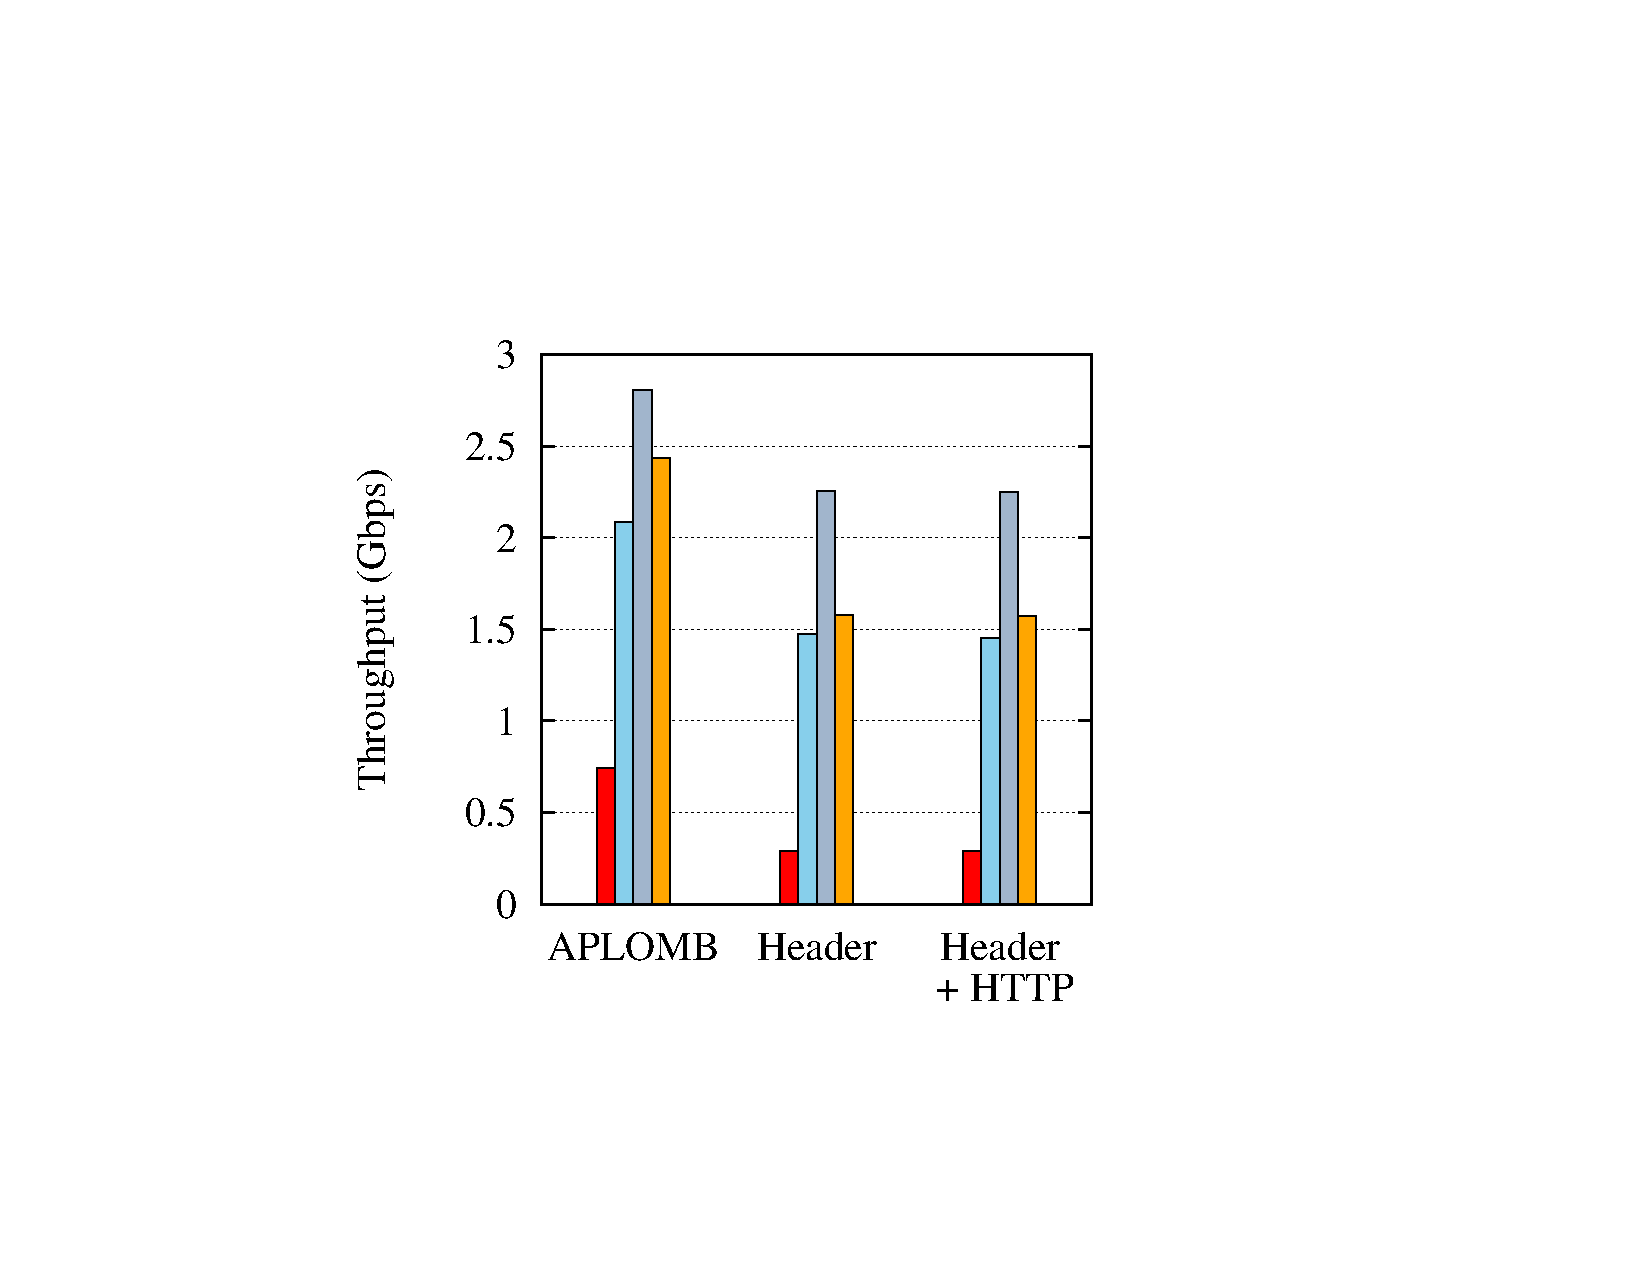
\includegraphics[height=1in]{fig/gatewayxput}%%%
\DIFdelendFL \DIFaddbeginFL 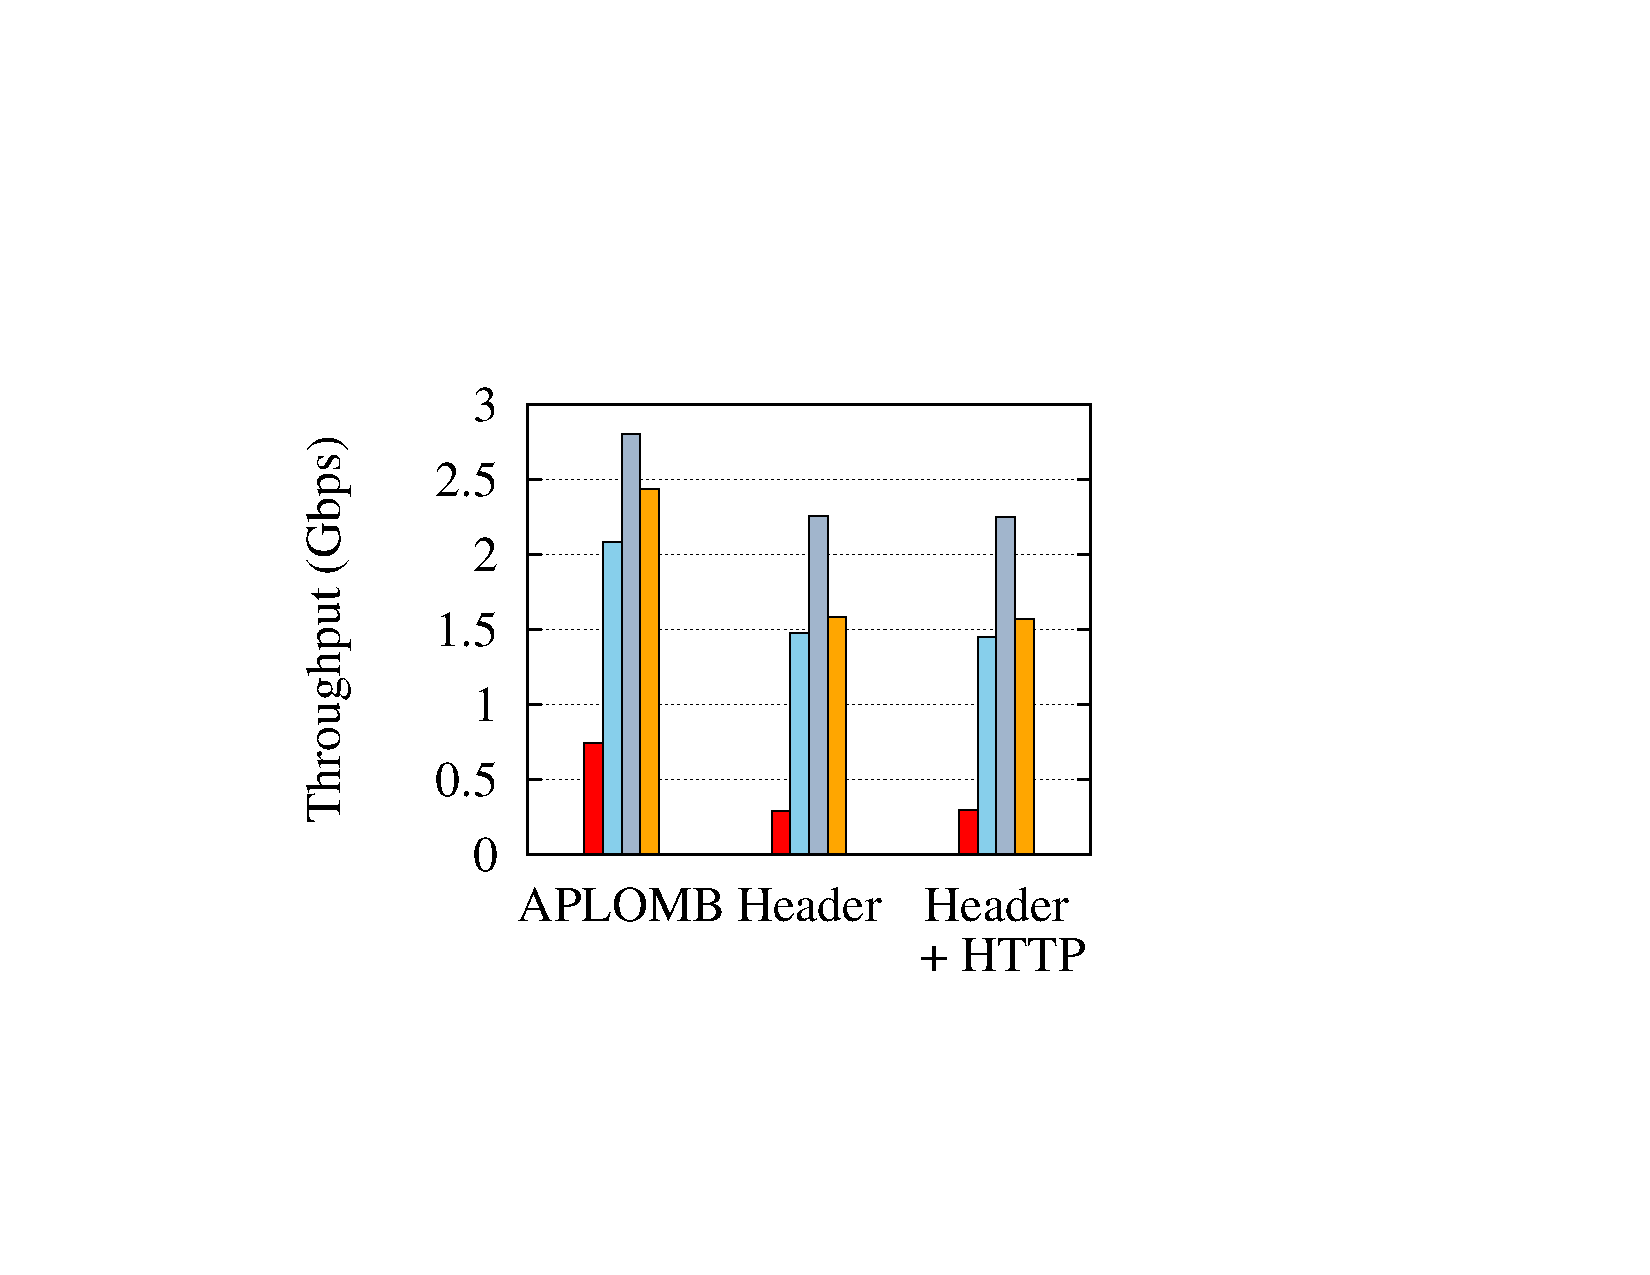
\includegraphics[height=1in]{fig/gateway_xput}\DIFaddendFL &
  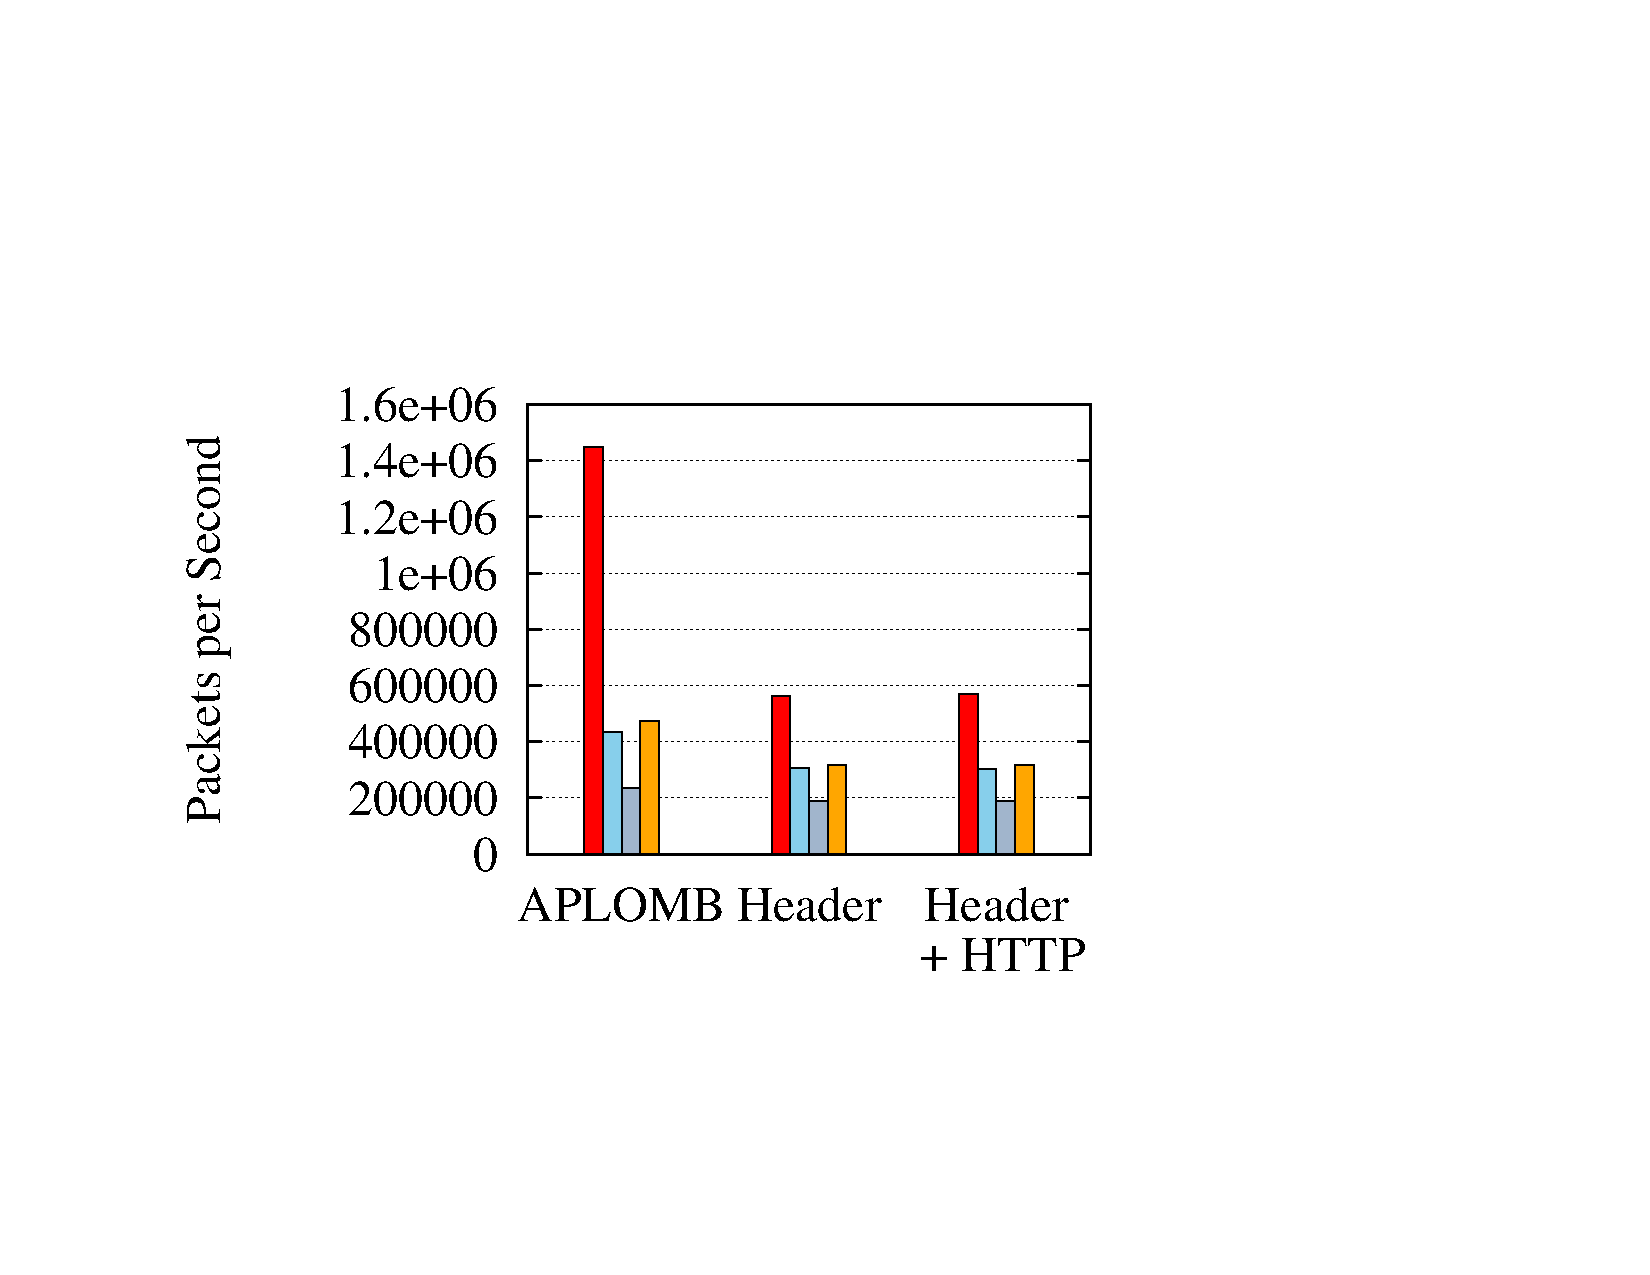
\includegraphics[height=1in]{fig/gateway_pps}\\
  \end{tabular}
  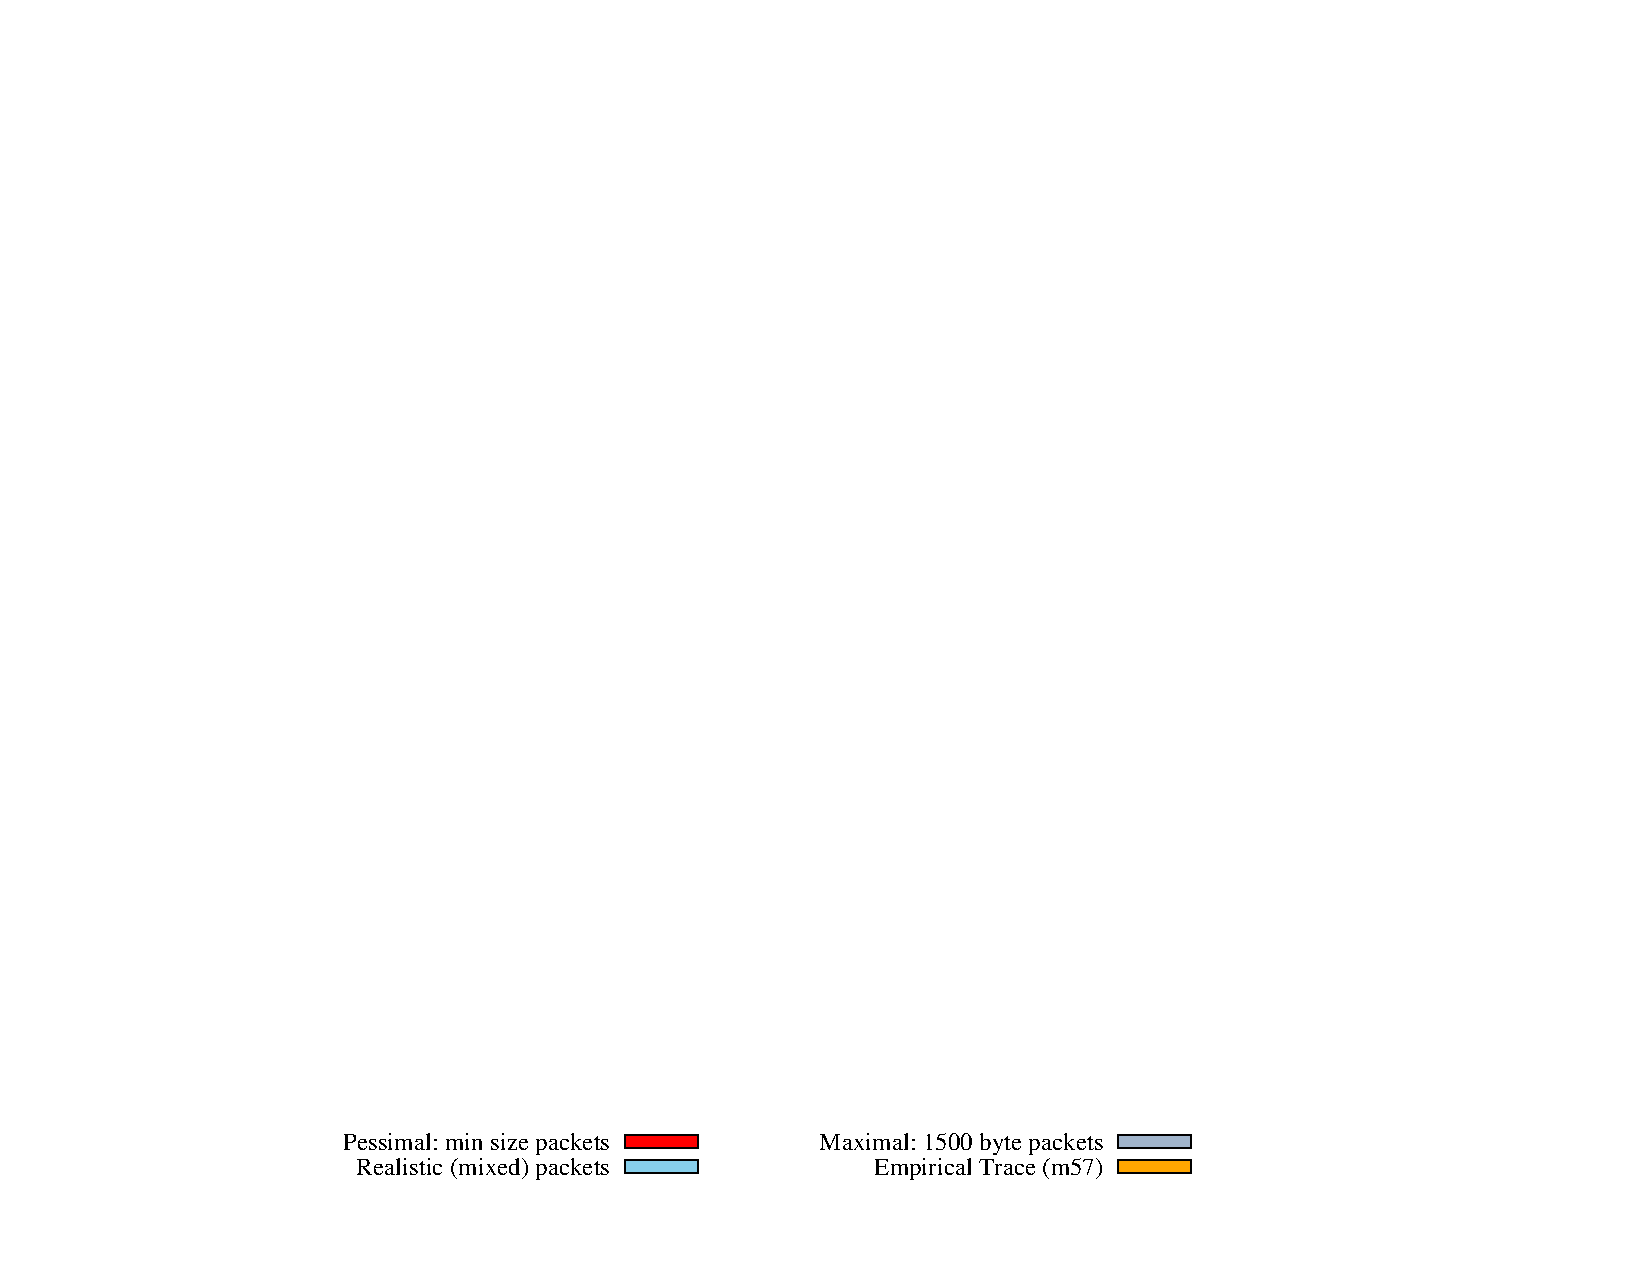
\includegraphics[width=2.75in]{fig/key}
  \caption[]{\label{fig:gwxput} Throughput on a single core at stateless gateway.}
\end{figure}

\begin{figure}[t]
  \centering
  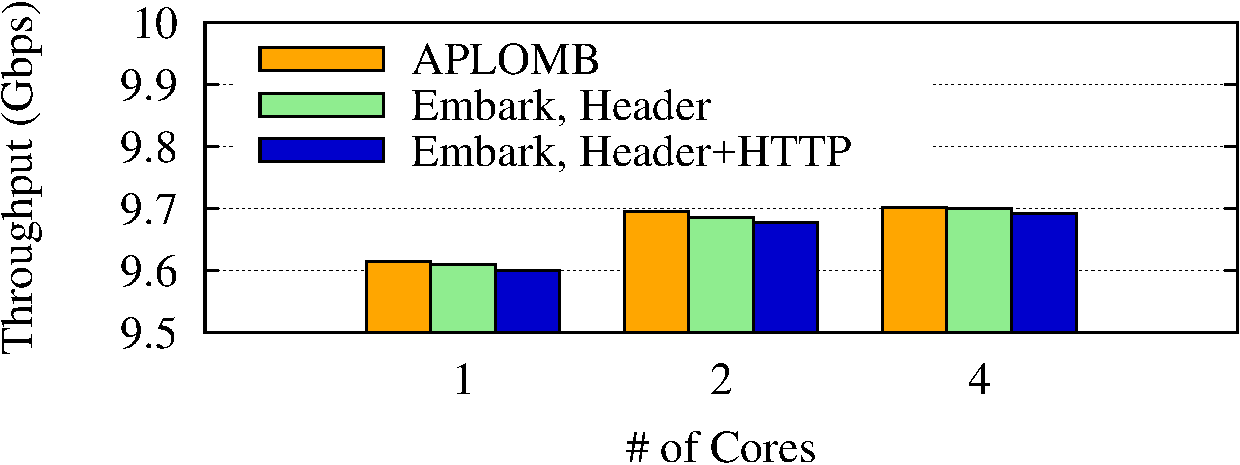
\includegraphics[width=2.8in]{fig/gateway_scale}
  \caption[]{\label{fig:gwscale} Gateway throughput with increasing parallelism.}
\end{figure}

\section{Evaluation} \label{sec:eval}

As we showed in \S\ref{sec:mbs}, \sys supports all middlebox applications in typical outsourcing environments~\cite{aplomb,etsi-nfv}. Hence, from a functionality perspective, \sys answers our original question, ``Is it possible to enable a third party to perform traffic processing for an enterprise, {\em without seeing the enterprise's traffic}?''  in the affirmative.

We now investigate whether \sys is practical from a performance perspective, looking at the overheads due to encryption and redirection. 
We built our gateway using Click~\cite{click} over DPDK~\cite{dpdk} on an off-the-shelf 16-core server with 2.6GHz Xeon E5-2650 cores and 128GB RAM; the network hardware is a single 10GbE Intel 82599 compatible network card. 
We deployed our prototype gateway in our research lab and redirected traffic from a 3-server testbed through the gateway; these three client servers had the same hardware specifications as the server we used as our gateway.
We deployed our middleboxes on Amazon EC2.
For most experiments, we use a synthetic workload generated by the Pktgen~\cite{pktgen}; for experiments where an empirical trace is specified we use the m57 patents trace~\cite{m57} and the ICTF 2010 trace~\cite{ictf}, both in IPv4.

%In what follows, we evaluate our performance at the enterprise, including gateway throughput, end-to-end page load times, and bandwidth costs (\S\ref{sec:enterprise}). We then evaluate performance at the cloud, evaluating each middlebox we implemented one by one (\S\ref{sec:evalcloud}).

\subsection{Enterprise Performance}
\label{sec:enterprise}
We first evaluate \sys's overheads at the enterprise. %including the gateway, end-to-end performance, and bandwidth costs from deploying \sys.

\subsubsection{Gateway}

 
\noindent{\it How many servers does a typical enterprise require to outsource traffic to the cloud?}
Figure~\ref{fig:gwxput} shows the gateway throughput when encrypting traffic to send to the cloud, first with normal redirection (as used in APLOMB~\cite{aplomb}), then with \sys's L3/L4-header encryption, and finally with L3/L4-header encryption as well as \DIFaddbegin \DIFadd{stateless }\DIFaddend HTTP/proxy encryption. 
For empirical traffic traces with payload encryption (DPI) disabled, \sys averages \DIFdelbegin \DIFdel{1.5}\DIFdelend \DIFaddbegin \DIFadd{9.6}\DIFaddend Gbps per core; for full-sized packets it achieves over \DIFdelbegin \DIFdel{2Gbps}\DIFdelend \DIFaddbegin \DIFadd{9.8Gbps}\DIFaddend .
In scalability experiments (Fig.~\ref{fig:gwscale}) with \DIFdelbegin \DIFdel{eight }\DIFdelend \DIFaddbegin \DIFadd{4 }\DIFaddend cores dedicated to processing, our server could could forward at up to \DIFdelbegin \DIFdel{8Gbps }\DIFdelend \DIFaddbegin \DIFadd{9.7Gbps for empirical traffic }\DIFaddend while encrypting for headers and HTTP traffic.
There is little difference between the HTTP overhead and the L3/L4 overhead, as the HTTP encryption only occurs on HTTP requests -- a small fraction of packets. 
With DPI enabled (not shown), throughput dropped to 240Mbps per core, suggesting that an enterprise would need to devote at least 32 cores to the gateway.
%Overall, \sys encryption for the stateless gateway reduces by about 60\% relative to baseline APLOMB encryption in the worst case (the min-sized workload; the reduction for the empirical (m57) workload is 38\%.  

\begin{figure}[t]
  \vspace{-10pt}
  \centering
  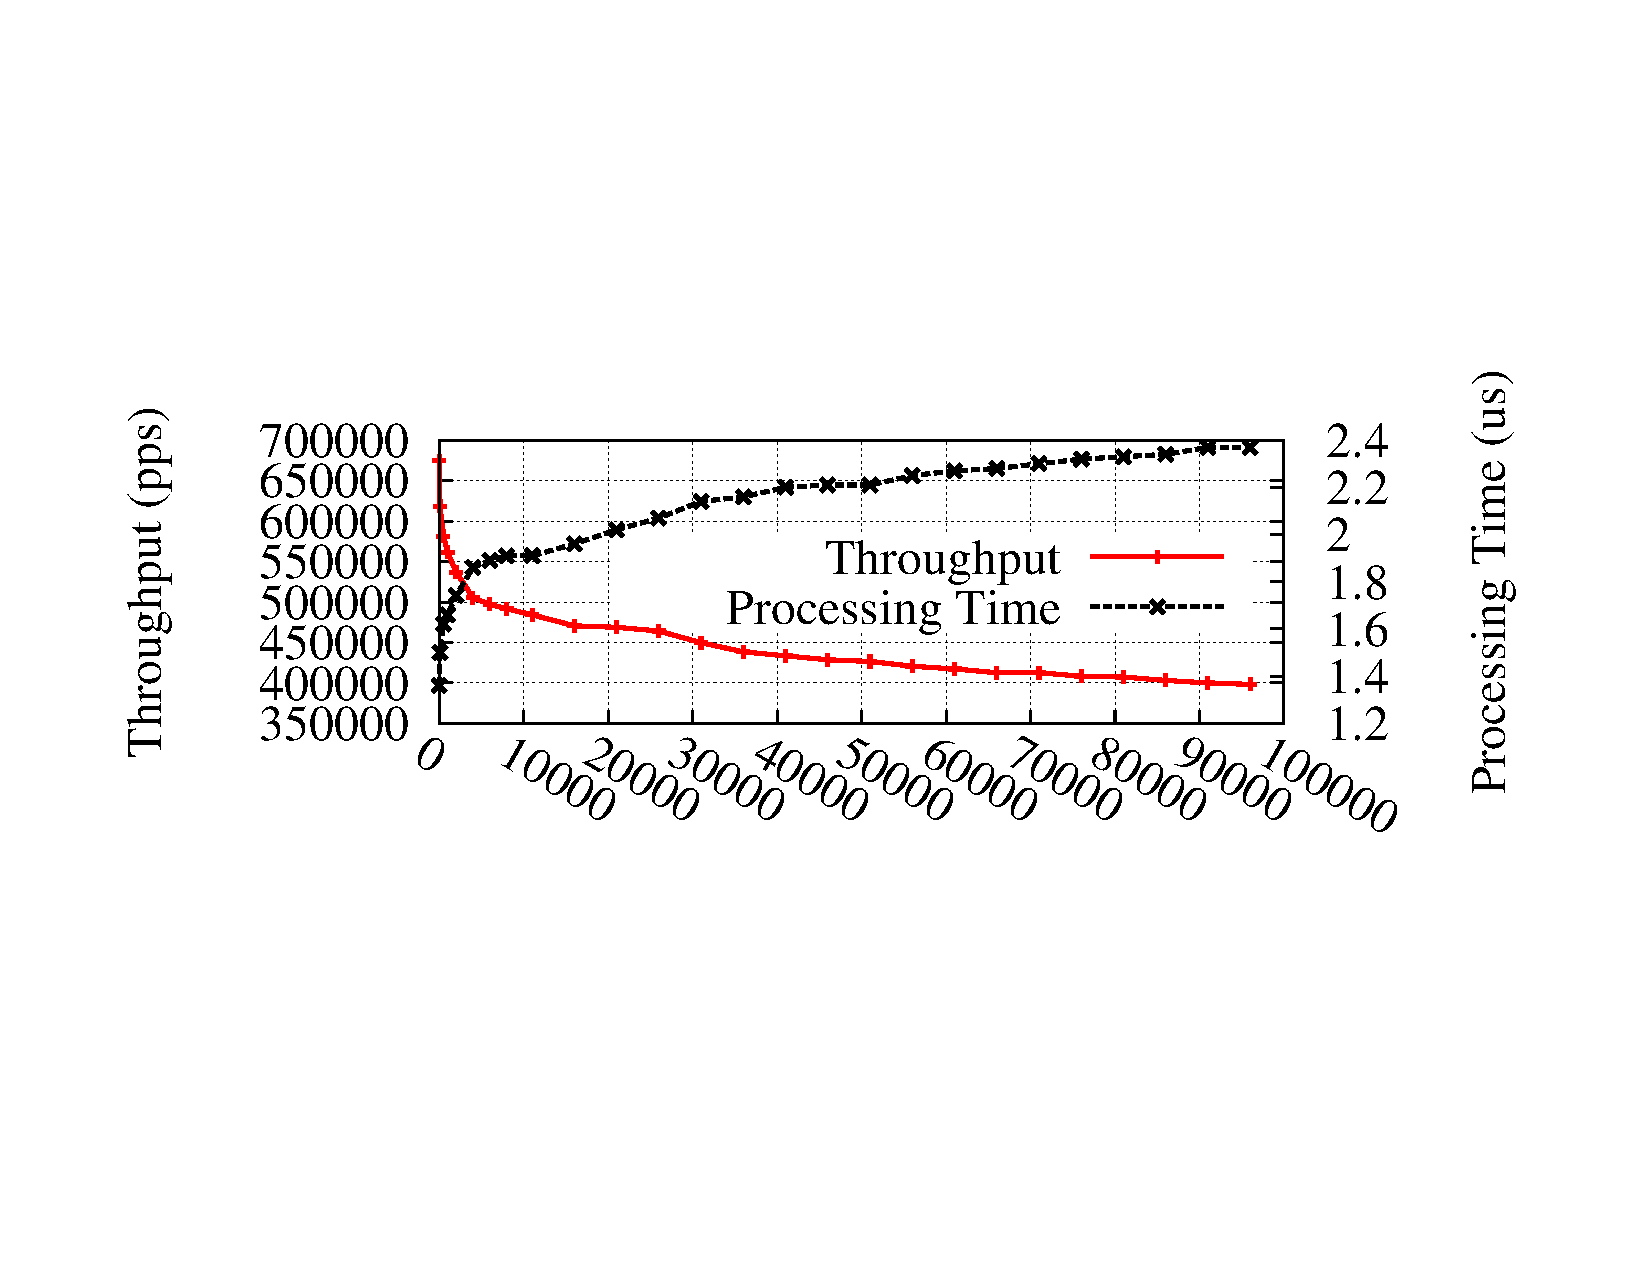
\includegraphics[width=3in]{fig/xputrange}
  \caption[]{\label{fig:xputrange} Throughput as \# of \DIFdelbeginFL \DIFdelFL{RangeMatch }\DIFdelendFL \DIFaddbeginFL \DIFaddFL{PrefixMatch }\DIFaddendFL rules increases.}
\end{figure}

\DIFdelbegin %DIFDELCMD < \noindent{\it How do throughput and latency at the gateway scale with the number of rules for RangeMatch?} 
%DIFDELCMD < %%%
\DIFdelend \DIFaddbegin \noindent{\it How do throughput and latency at the gateway scale with the number of rules for PrefixMatch?} 
\DIFaddend In \S\ref{sec:range}, we discussed how \DIFdelbegin \DIFdel{RangeMatch stores encrypted values in a tree}\DIFdelend \DIFaddbegin \DIFadd{PrefixMatch stores sorted intervals}\DIFaddend ; every packet encryption requires a \DIFdelbegin \DIFdel{traversal of this tree}\DIFdelend \DIFaddbegin \DIFadd{binary search of intervals}\DIFaddend . Hence, as the size of the tree goes larger, we can expect to require more time to process each packet and throughput to decrease. We measure this effect in Figure~\ref{fig:xputrange}. 
On the $y_1$ axis, we show the aggregate per packet throughput at the gateway as the number of rules from 0 to 100k. The penalty here is logarithmic, which is the expected performance of tree data structures. From 0-10k rules, throughput drops from \DIFdelbegin \DIFdel{670Kpps to 480Kpps}\DIFdelend \DIFaddbegin \DIFadd{3Mpps to 1.5Mpps}\DIFaddend ; after this point the performance penalty of additional rules tapers off. Adding an additional 90k rules drops throughput to \DIFdelbegin \DIFdel{400Kpps}\DIFdelend \DIFaddbegin \DIFadd{1.1Mpps}\DIFaddend .
On the $y_2$ axis, we measure the processing time per packet, \ie{}, the amount of time for the gateway to encrypt the packet; the processing time follows the same logarithmic trend.

\DIFdelbegin %DIFDELCMD < \noindent{\it Is RangeMatch faster than existing order preserving algorithms?}
%DIFDELCMD < %%%
\DIFdel{RangeMatch }\DIFdelend \DIFaddbegin \noindent{\it Is PrefixMatch faster than existing order preserving algorithms?}
\DIFadd{PrefixMatch }\DIFaddend is the only encryption scheme that has low latency and the ordering property needed for packet processing.
We compare against BCLO~\cite{boldyreva:ope} and mOPE~\cite{popa:mope} below:

\begin{table}[h]
\vspace{-10pt}
\centering
\small
\begin{tabular}{c|c|c|c}
{\bf Operation}&{\bf BCLO}&{\bf mOPE}&{\bf \sys}\\
\hline
\hline
Encrypt, 10K rules&9333$\mu$s&6640$\mu$s&\DIFdelbeginFL \DIFdelFL{1.95}\DIFdelendFL \DIFaddbeginFL \DIFaddFL{0.53}\DIFaddendFL $\mu$s\\
\hline
Encrypt, 100K rules&9333$\mu$s&8300$\mu$s&\DIFdelbeginFL \DIFdelFL{3}\DIFdelendFL \DIFaddbeginFL \DIFaddFL{0.77}\DIFaddendFL $\mu$s\\
\hline
Decrypt&169$\mu$s&0.128$\mu$s&0.128$\mu$s\\
\hline
\end{tabular}
\vspace{-10pt}
\end{table}

\DIFdelbegin %DIFDELCMD < \noindent{\it What is the memory overhead of RangeMatch?}
%DIFDELCMD < %%%
\DIFdelend \DIFaddbegin \noindent{\it What is the memory overhead of PrefixMatch?}
\DIFaddend Storing 10k rules in memory requires 1.6MB, and storing 100k rules in memory requires 28.5MB -- using unoptimized C++ objects.
This overhead is negligible.% on any modern server.

\subsubsection{Client Performance}

\begin{figure}
  \vspace{-10pt}
  \hspace{-15pt}
%  \begin{tabular}{cccc}
%  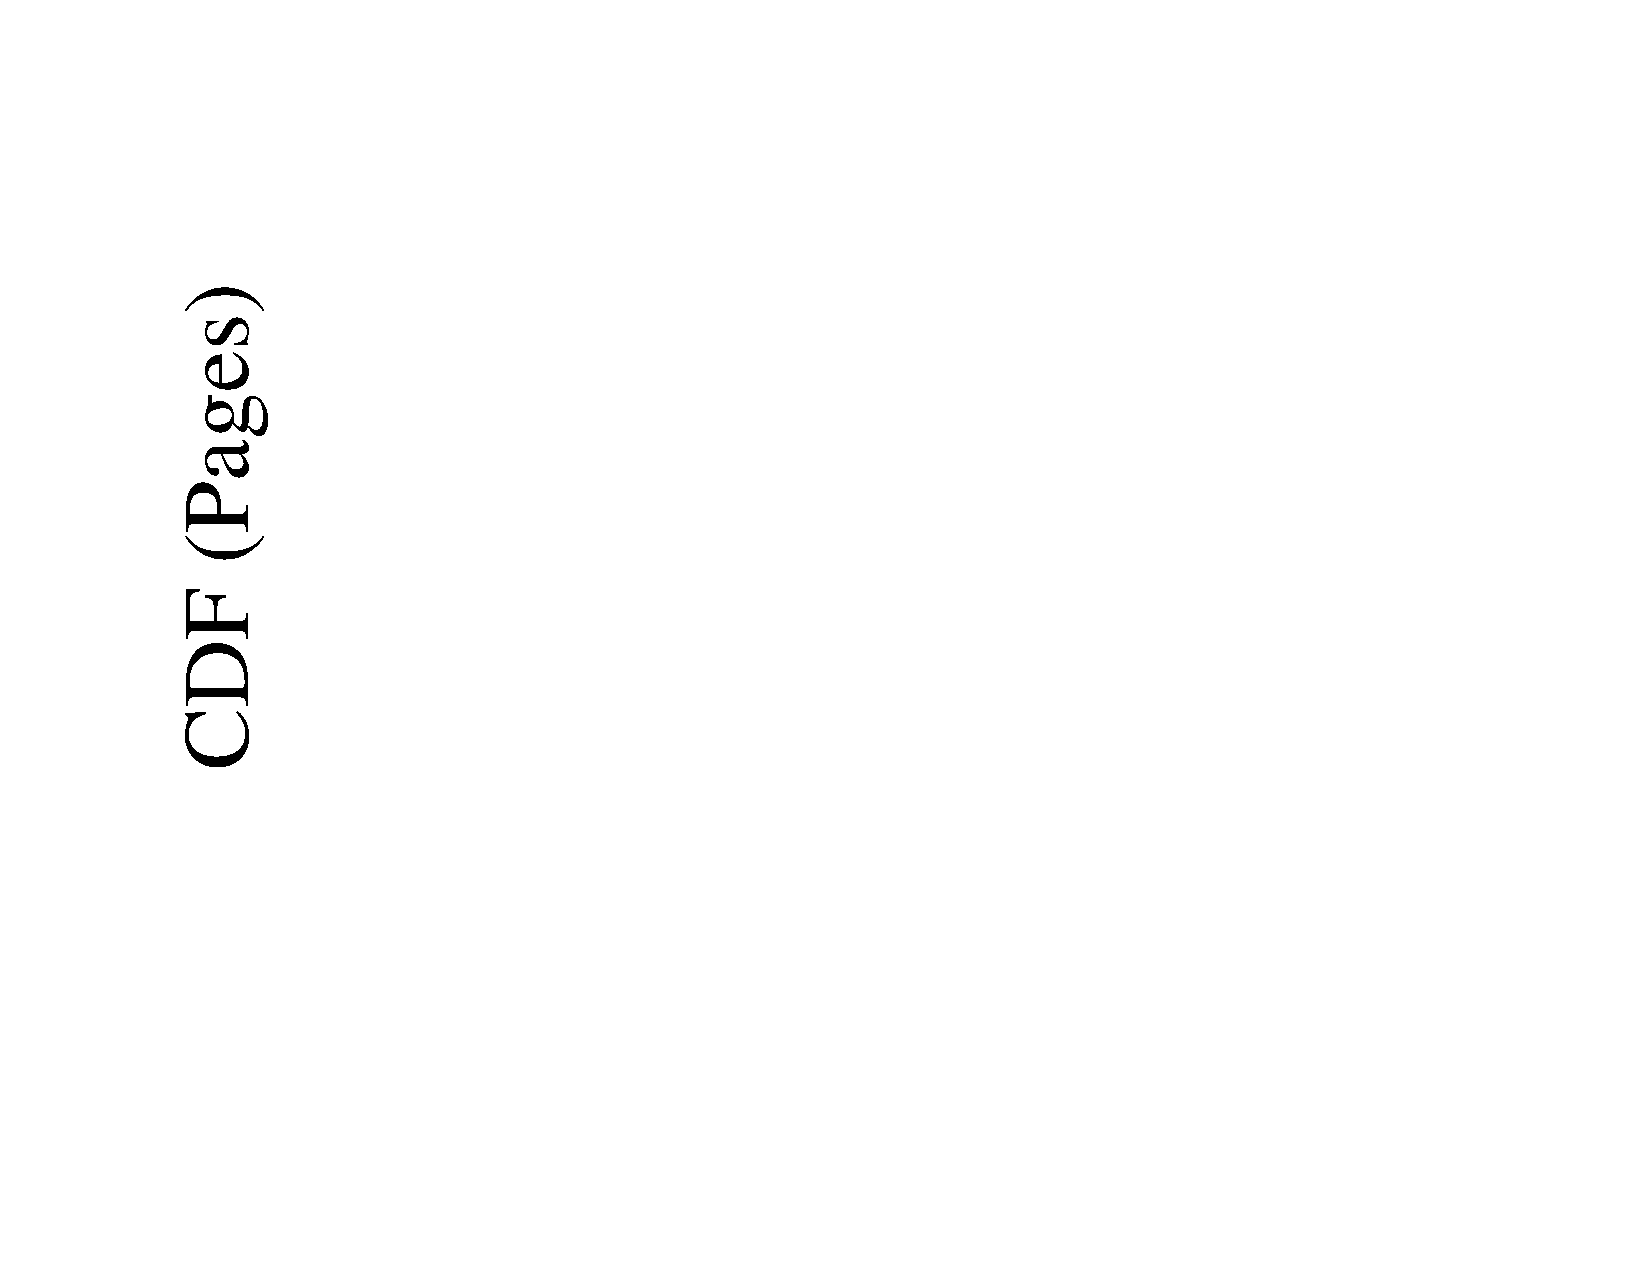
\includegraphics[height=1in]{fig/cdflabel}
%  &\hspace{-10pt}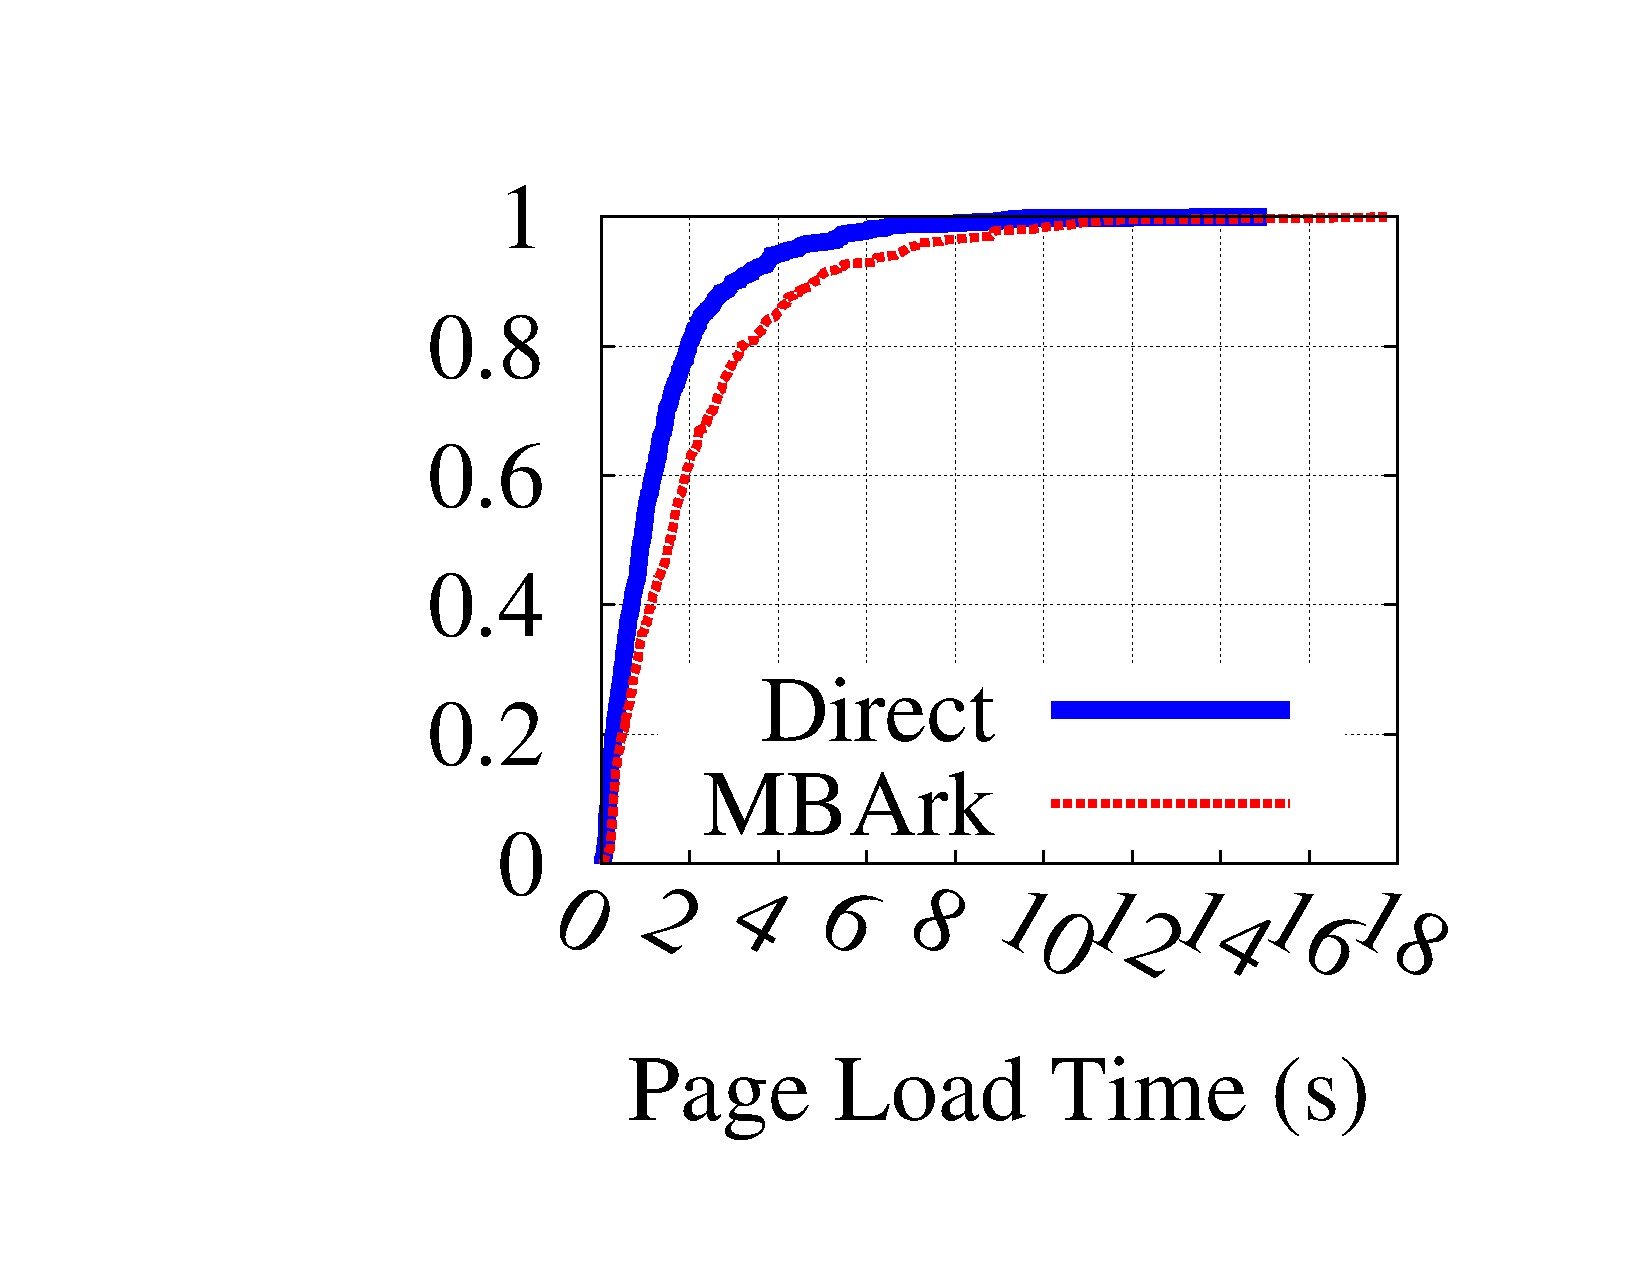
\includegraphics[height=.9in]{fig/e2e_loadtimes}
%  &\hspace{-10pt}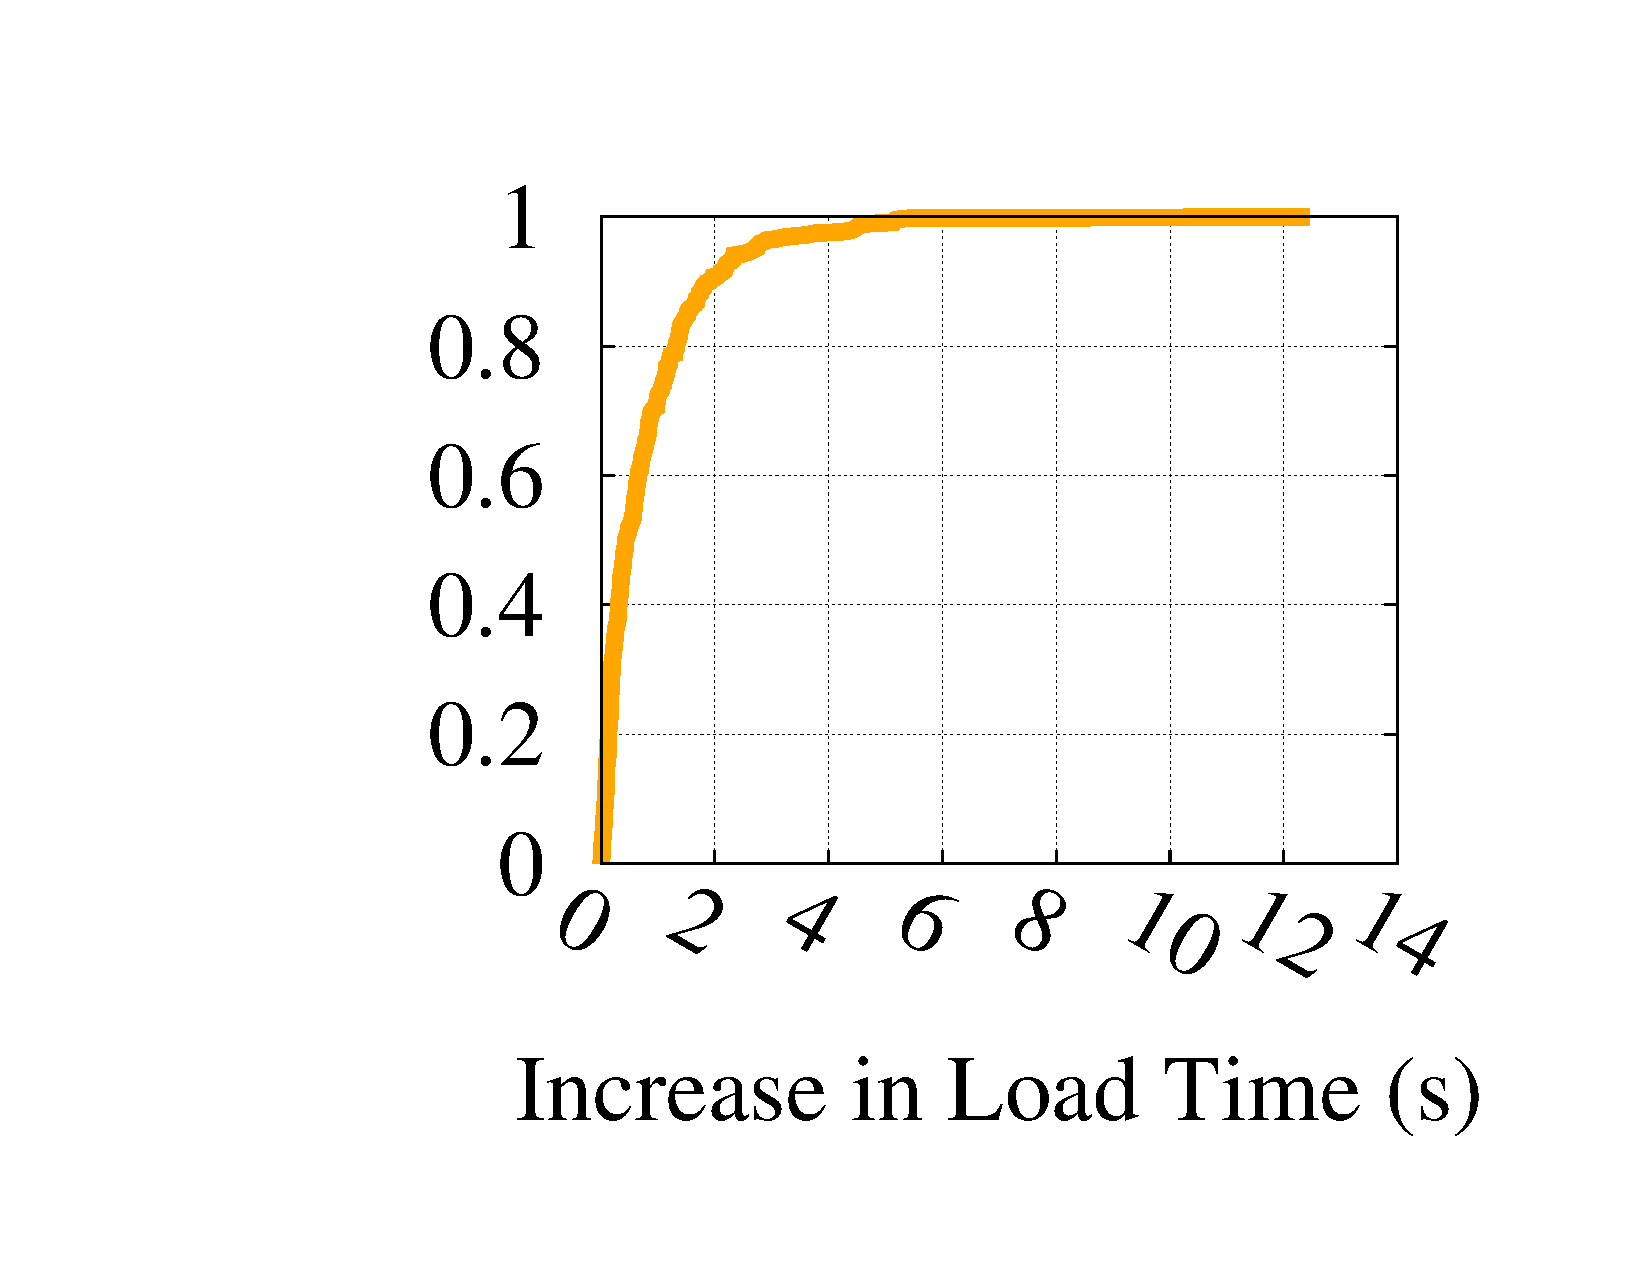
\includegraphics[height=.9in]{fig/e2e_delta_absolute}
%  &\hspace{-10pt}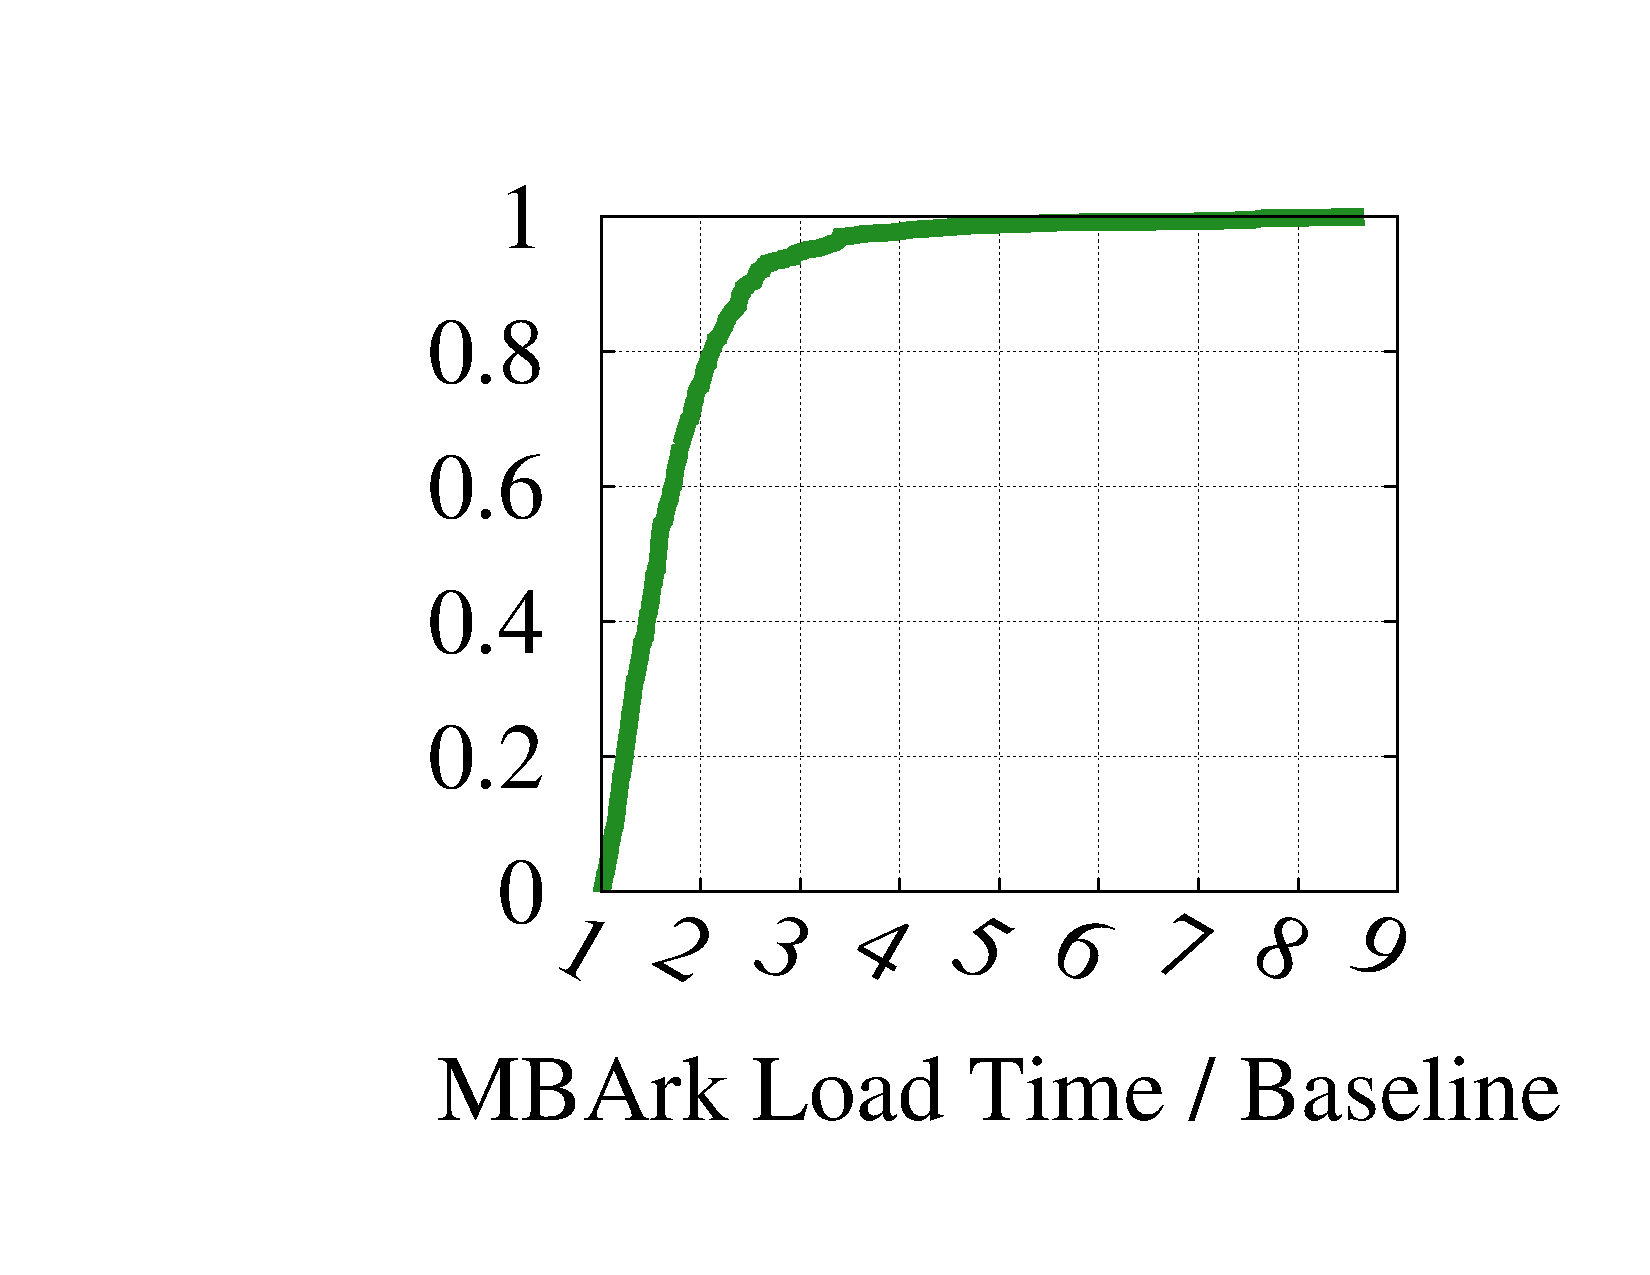
\includegraphics[height=.9in]{fig/e2e_delta_relative}
%  \\
%  &(a)&(b)&(c)\\
%  \end{tabular}
  \centering
  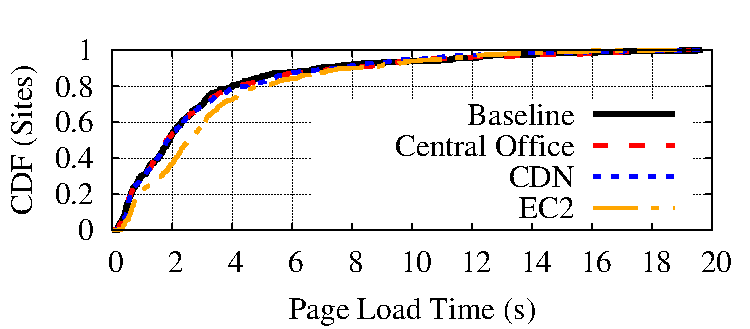
\includegraphics[width=2.7in]{fig/e2e_compare}
  \caption[]{\label{fig:e2eloads} Page load times under different deployments.}
\end{figure}

We use web performance to understand end-to-end user experience of \sys.
Figure~\ref{fig:e2eloads} shows a CDF for the Alexa top-500 sites loaded through our testbed. We compare the baseline (direct download) assuming three different service providers: an ISP hosting services in a Central Office (CO), a Content-Distribution Network, and a traditional cloud provider (EC2). The mean RTTs from the gateway are 60$\mu$s, 4ms, and 31ms, respectively. We deployed \sys on EC2 and used this deployment for our experiments, but for the CO and CDN we emulated the deployment with inflated latencies and servers in our testbed. We ran a pipeline of NAT, firewall and proxy (with empty cache) in the experiment.
Because of the `bounce' redirection \sys uses, all page load times increase by some fraction; in the median case this increase is less than 50ms for the ISP/Central Office, 100ms for the CDN, and 720ms using EC2; hence ISP \DIFdelbegin \DIFdel{and CDN }\DIFdelend based deployments will escape human perception~\cite{millishumans} but a \DIFdelbegin \DIFdel{cloud deployment will }\DIFdelend \DIFaddbegin \DIFadd{CDN (or a cloud deployment) may }\DIFaddend introduce human-noticeable overheads.

\subsubsection{Bandwidth Overheads}
We evaluate two costs: the increase in bandwidth due to our encryption and metadata, and the increase in bandwidth cost due to `bounce' redirection.

\noindent{\it How much does \sys encryption increase the amount of data sent to the cloud?}
The gateway inflates the size of traffic due to three encryption costs:
\begin{myitemize}
  \item If the enterprise uses IPv4, there is a 20-byte per-packet cost to convert from IPv4 to IPv6. If the enterprise uses IPv6 by default, there is no such cost.
  \item If HTTP proxying is enabled, there are on average 132 bytes per request in additional encrypted data.
  \item If HTTP IDS is enabled, there is at worst a 5$\times$ overhead on all HTTP payloads~\cite{blindbox}.
\end{myitemize}
We used the m57 trace to understand how these overheads would play out in aggregate for an enterprise.
On the uplink, from the gateway to the middlebox service provider, traffic would increase by 2.5\% due to encryption costs for a header-only gateway. Traffic would increase by 4.3$\times$ on the uplink for a gateway that supports DPI middleboxes. 

\noindent{\it How much does bandwidth increase between the gateway and the cloud from using \sys? How much would this bandwidth increase an enterprises networking costs?}
\sys sends all network traffic to and from the middlebox service provider for processing, before sending that traffic out to the Internet at large. 

In ISP contexts, the clients' middlebox service provider and network connectivity provider are one and the same and one might expect costs for relaying the traffic to and from the middleboxes to be rolled in to one service `package;' given the latency benefits of deployment at central offices (as we saw in Fig.~\ref{fig:e2eloads}) we expect that ISP-based deployments are the best option to deploy \sys.

In the cloud service setting the client must pay a third party ISP to transfer the data to and from the cloud, before paying that ISP a third time actually transfer the data over the network.
Using current US bandwidth pricing~\cite{comcast-costs, megapath-costs, verizon-costs}, we can estimate how much outsourcing would increase overall bandwidth costs.
Multi-site enterprises typically provision two kinds of networking costs: Internet access, and intra-domain connectivity. 
Internet access typically has high bandwidth but a lower SLA; traffic may also be sent over shared Ethernet~\cite{comcast-costs, verizon-costs}.
Intra-domain connectivity usually has a private, virtual Ethernet link between sites of the company with a high SLA and lower bandwidth.
Because bounce redirection is over the `cheaper' link, the overall impact to bandwidth cost with header-only encryption given public sales numbers is between 15-50\%; with DPI encryption this cost increases to between 30-150\%. 

%DIF < Getting frustrated with these numbers so leaving them here and will come back to them. Megapath offers a dedicated link at 5x5Mbps for \$250/mo; 20x20Mbps for \$1300/mo. Comcast offers enterprise cable at 150/20Mbps for \$250/mo. The three way bounce should result in a cost increase of 15-50\%, depending on how much the internal link is provisioned for. The DPI should be 2-3 times that, so, between 30-150\%... 
%DIF > \eat{Getting frustrated with these numbers so leaving them here and will come back to them. Megapath offers a dedicated link at 5x5Mbps for \$250/mo; 20x20Mbps for \$1300/mo. Comcast offers enterprise cable at 150/20Mbps for \$250/mo. The three way bounce should result in a cost increase of 15-50\%, depending on how much the internal link is provisioned for. The DPI should be 2-3 times that, so, between 30-150\%... 
%DIF > }

\subsection{Middleboxes}
\label{sec:evalcloud}

We now evaluate the overheads at each middlebox. 

\begin{table}[t!]
\small
\begin{tabular}{p{2.5cm}|p{2cm}|p{2cm}}
{\bf Application} &  {\bf Baseline Throughput} & {\bf \sys Throughput} \\
\hline \hline
IP Firewall &  9.8Gbps &  9.8Gbps \\
%Application Firewall  & & \\
NAT & 3.6Gbps   &   3.5 Gbps \\
%IP Forwarding  & & \\
%VPN Gateway &  &  &  \\ 
Load Balancer L4  &9.8 Gbps & 9.8Gbps \\
%Load Balancer L7 & & & \\
%WAN optimizer  & & & \\
Web Proxy &1.1Gbps &1.1Gbps\\
%IDS & & & \\
IDS & 85Mbps & 166Mbps~\cite{blindbox}   \\
\end{tabular}
\caption{Middlebox throughput for an empirical workload. \label{tbl:appsxput}}
\DIFdelbeginFL %DIFDELCMD < \vspace{-5pt}
%DIFDELCMD < %%%
\DIFdelendFL \end{table}

\noindent{\it Is throughput reduced at the middleboxes due to  \sys?}
\DIFaddbegin 

\DIFaddend Table~\ref{tbl:appsxput} shows the throughput sustained for the apps we implemented.
The IP Firewall, NAT, and Load Balancer are all `header only' middleboxes; the results shown compare packet processing over the same dataplane, once with encrypted IPv6 data and once with unencrypted IPv4 data.
The only middlebox for which any overhead is observable is the NAT -- and this is a reduction of only 2.7\%.

We re-implemented the Web Proxy and IDS to enable the bytestream aware operations they require over our encrypted data. We compare our Web Proxy implementation with Squid~\cite{squid}. The Web Proxy sustains the same throughput with and without encrypted data, but, as we will present later, does have a higher service time per cache hit.
The IDS numbers compare Snort (baseline) to the BlindBox implementation; this is not an apples-to-apples comparison as BlindBox performs mostly exact matches where Snort matches regular expressions.

In what follows, we provide some further middlebox-specific benchmarks for the firewall, proxy, and IDS.

\noindent{\bf Firewalls:} 
{\it Does \sys support all rules in a typical firewall configuration? How much does the ruleset ``expand'' due to encryption?}
\DIFaddbegin 

\DIFaddend We tested our firewall with three rulesets provided to us by a network administrator at our institution \DIFaddbegin \DIFadd{and an IP firewall ruleset from Emerging Threats~\mbox{%DIFAUXCMD
\cite{emergingthreats}}%DIFAUXCMD
}\DIFaddend . We were able to encode all rules using range and keyword match encryptions. \DIFaddbegin \DIFadd{The size of 3 rulesets did not change after encryption, while the size of the other ruleset from Emerging Threats expanded from 1363 to 1370 -- a 0.5\% increase. Therefore we conclude that it has negligible impact on the firewall performance.
}\DIFaddend 


\DIFdelbegin \DIFdel{We also investigated how much the ruleset increased due to RangeMatch. Rules are typically encoded in the firewall as prefixes, hence a rule over the range }%DIFDELCMD < [%%%
\DIFdel{4.0.0.0, 4.255.255.255}%DIFDELCMD < ] %%%
\DIFdel{is in practice implemented as a bit-mask over the first 8 bits of every packet.
Using RangeMatch, the same prefix might be mapped to 9.128.0.0-10.128.0.0.0, resulting in two /9 prefix ranges in the final rule encoding: 9.128.0.0/9 or 10.128.0.0/9.
As throughput for many middleboxes decreases with the number of rules, we were concerned that these mappings might degrade performance.
However, in practice rules increased modestly, by between 5.8\% and 10.2\%.
}\DIFdelend %DIF >  We also investigated how much the ruleset increased due to PrefixMatch. Rules are typically encoded in the firewall as prefixes, hence a rule over the range [4.0.0.0, 4.255.255.255] is in practice implemented as a bit-mask over the first 8 bits of every packet. Using PrefixMatch, the same prefix might be mapped to 9.128.0.0-10.128.0.0.0, resulting in two /9 prefix ranges in the final rule encoding: 9.128.0.0/9 or 10.128.0.0/9. As throughput for many middleboxes decreases with the number of rules, we were concerned that these mappings might degrade performance. However, in practice rules increased modestly, by between 5.8\% and 10.2\%.

\begin{figure}[t]
\centering
\DIFdelbeginFL %DIFDELCMD < \vspace{-10pt}
%DIFDELCMD < %%%
\DIFdelendFL 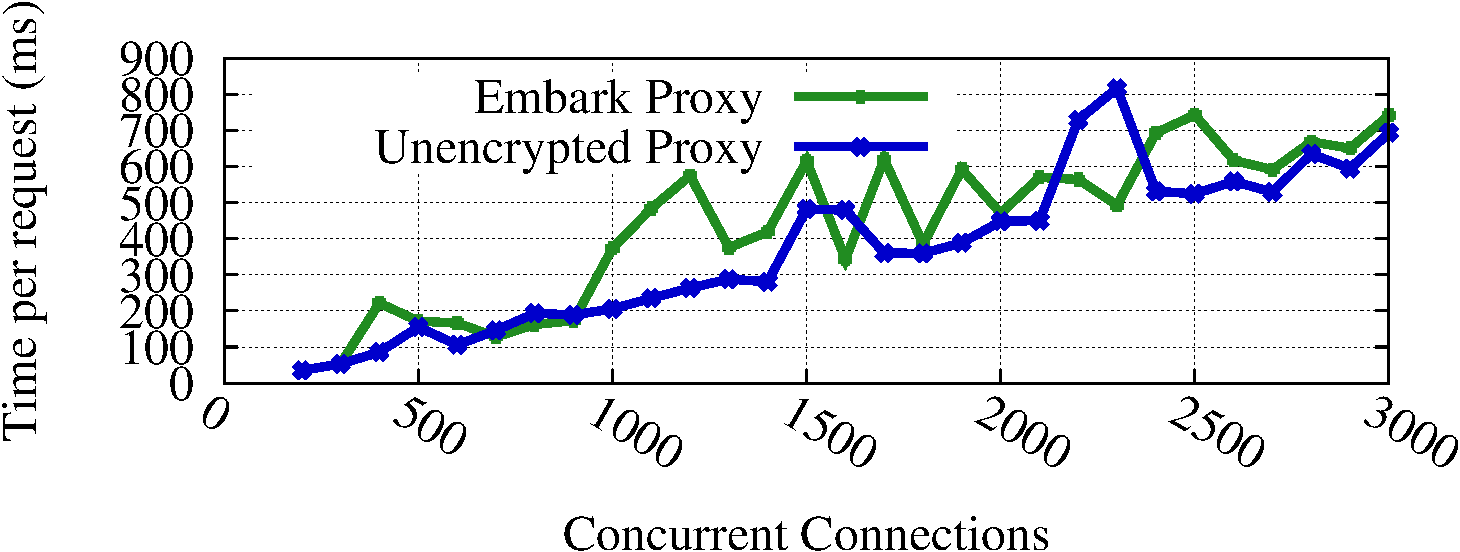
\includegraphics[width=3in]{fig/proxytime}
\caption{\label{fig:proxygraph} Access time per page against the number of concurrent connections at the proxy.}
\end{figure}

\noindent{\bf Proxy/Caching:} The throughput number shown in Table~\ref{tbl:appsxput} is not the typical metric used to measure proxy performance. A better metric for proxies is how many connections the proxy can handle concurrently, and what time-to-service it offers each client. In Figure~\ref{fig:proxygraph}, we plot time-to-service against the number of concurrent connections, and see that it is on average higher for \sys than the unencrypted proxy, by tens to hundreds of milliseconds per page.
This is not due to computation costs, but instead, due to the fact that the encrypted HTTP header values are transmitted on a different channel than the primary data connection.
The \sys proxy needs to synchronize between these two flows; this synchronization cost is what increases the time to service. 


\noindent{\bf Intrusion Detection:}
Our IDS is based on BlindBox~\cite{blindbox}. BlindBox incurs a substantial `setup cost' every time a client initiates a new connection. With \sys, however, the gateway and the cloud maintain one, long-term persistent connection. 
Hence, this setup cost is paid once when the gateway is initially configured. \sys also heuristically expands regular expressions in the rulesets into exact match strings. This results in two benefits:

\DIFdelbegin %DIFDELCMD < \noindent{\it (1) End-to-end performance improves.} %%%
\DIFdelend \DIFaddbegin \noindent{\it (1) End-to-end performance improvements.} \DIFaddend Where BlindBox incurs an initial handshake of 414s~\cite{blindbox} to open a new connection, clients under \sys never pay this cost; instead they perform a normal TCP or SSL handshake of only 3-5 RTTs. In our testbed, this amounts to between 30 and 100 ms, depending on the site and protocol -- an improvement of 4 orders of magnitude.

\noindent{\it (2) Security improvements.} 
Using IDS rulesets from Snort, we converted regular expressions to exact match strings as discussed in \S\ref{sec:bbarch}. With 10G memory, we were able to convert about half of all regular expressions to a finite number of exact match strings; the remainder resulted in too many possible states. 
We used two rulesets to evaluate this~\cite{emergingthreats, snort-community}. With the first ruleset BlindBox would resort to the lower security level for 33\% of rules, but \sys would only require this for 11.3\%. With the second ruleset, BlindBox would use lower security for 58\% of rules, but \sys would only do so for 20.2\%. \DIFaddbegin \DIFadd{The major drawback of }\sys \DIFadd{is that }\sys \DIFadd{cannot perform probable cause encryption, because there is no end-to-end SSL session in the }\sys \DIFadd{scenario. However, }\sys \DIFadd{still strictly improves the security in this outsourcing scenario.
}\DIFaddend 

%DIF > \eat{
%\begin{table}[h]
%  \centering
%  \small
%  \begin{tabular}{l|c|c}
%  %\begin{tabular}{p{1.75in}|p{.4in}|p{.4in}}
%    {{\bf Rule Set}}&{\bf Exact Match}&{\bf Prob. Cause}\\
%    \hline
%    \hline
%    BB: Community&67\%&100\%\\
%    \hline
%    MB: Community&88.7\%&100\%\\
%DIF > 
%    \hline
%    \hline
%    BB: Emerging Threats&42\%&100\%\\
%    \hline
%    MB: Emerging Threats&79.8\%&100\%\\
%    \hline
%  \end{tabular}
%\end{table}
%DIF > }


%!TEX root = mb.tex

\section{Related Work}
\label{sec:related}

\noindent{\bf Middlebox Outsourcing:}
APLOMB~\cite{aplomb} is a practical service for outsourcing enterprise's middleboxes to the cloud, which we discussed in detail in \S\ref{sec:overview}.

\noindent{\bf Data Confidentiality:}
Confidentiality of data in the cloud has been widely recognized as an important problem and researchers proposed solutions for software~\cite{Baumann:Haven}, web applications \cite{giffin:hails, Mylar},  filesystems~\cite{blaze:cfs, kallahalla:plutus, goh:sirius},  databases~\DIFdelbegin \DIFdel{\mbox{%DIFAUXCMD
\cite{popa:cryptdb}}%DIFAUXCMD
}\DIFdelend \DIFaddbegin \DIFadd{\mbox{%DIFAUXCMD
\cite{popa:cryptdb, blindseer}}%DIFAUXCMD
}\DIFaddend ,  and virtual machines~\cite{Zhang:CloudVisor}. 
CryptDB~\cite{popa:cryptdb} was one of the first practical systems to compute on encrypted data, but none of its encryption schemes or database system design apply to our network setting. 

Focusing on traffic processing, the most closely related work to \sys is BlindBox~\cite{blindbox}, discussed in \S\ref{sec:overview}.  mcTLS~\cite{mctls} proposed a protocol in which client and server can jointly authorize a middlebox to process certain portions of the encrypted traffic. Unlike \sys, the middlebox  gains access to unencrypted data and is still able to leak that data should it choose to do so. \DIFaddbegin \DIFadd{A recent paper~\mbox{%DIFAUXCMD
\cite{secmb} }%DIFAUXCMD
proposed a system architecture for outsourced middleboxes to specifically perform deep packet inspection over encrypted traffic.
}\DIFaddend 

\noindent{\bf Trace Anonymization and Inference:}
Some systems which focus on {\it offline} processing allow some analysis over anonymized data \cite{Vern:Anonymize06, Vern:Anonymize03}; they are not suitable for online processing as is \sys.
Yamada et al~\cite{Yamada_IDS} show how one can perform some very limited processing on an SSL-encrypted packet by using only the size of data and the timing of packets, however they cannot perform analysis of the contents of connection data.

\noindent{\bf Encryption Schemes:}
\sys's \DIFdelbegin \DIFdel{RangeMatch }\DIFdelend \DIFaddbegin \DIFadd{PrefixMatch }\DIFaddend scheme is similar to order preserving encryption schemes, but no existing scheme provided both the performance and security properties we required.
The order-preserving encryption~\cite{boldyreva:ope, popa:mope} used in CryptDB is 
 \DIFdelbegin \DIFdel{$>3000$ }\DIFdelend \DIFaddbegin \DIFadd{$>10000$ }\DIFaddend times slower than \DIFdelbegin \DIFdel{RangeMatch }\DIFdelend \DIFaddbegin \DIFadd{PrefixMatch }\DIFaddend (\S\ref{sec:eval}); moreover, it leaks the order of the IP addresses encrypted, while \DIFdelbegin \DIFdel{RangeMatch }\DIFdelend \DIFaddbegin \DIFadd{PrefixMatch }\DIFaddend protects this information. \DIFaddbegin \DIFadd{However, OPE schemes are more generic and applicable to a wide set of scenarios. PrefixMatch, on the other hand, is designed for a particular scenario.
}\DIFaddend The encryption scheme of Boneh et al.~\cite{BonehRange} enables detecting if an encrypted value matches a range and provides a similar security guarantee to \DIFdelbegin \DIFdel{RangeMatch}\DIFdelend \DIFaddbegin \DIFadd{PrefixMatch}\DIFaddend ; but, it is orders of magnitude slower than the OPE schemes which are already \DIFdelbegin \DIFdel{3000}\DIFdelend \DIFaddbegin \DIFadd{10000}\DIFaddend $\times$ slower than \DIFdelbegin \DIFdel{RangeMatch}\DIFdelend \DIFaddbegin \DIFadd{PrefixMatch}\DIFaddend . 

%  mOPE unfortunately requires that the gateway and the service provider interact for a number of roundtrips (e.g., xxx in our experiments) which is too slow and requires additional setup for this interaction, and violates requirement~\ref{req:sec} or~\ref{req:injective}, and BCLO has weak security (leaking always the top half bits of the values encrypted and the order of IP addresses across different packets, thus violating requirement~\ref{req:sec}), is too slow, and not format-preserving. 

% HERE ARE A FEW USEFUL NOTES ABOUT HOW OUR DESIGN IS DIFFERENT FROM mOPE -- THERE IS SOME SIMILARITY DUE TO TREE AND ADJUST
% we do not readjust for encryption 
% - this is expensive, we do not leak data between two encryptions 
% The tree is stored at the gateway. The tree contains as nodes the ends of the intervals as opposed to all values encoded-- thus, the tree is much smaller. firewalls have on the order of thousands such rules, so the tree is not large. also store only ranges and not everything encoded, making it smaller and fit into the gateway, etc., they need adjustments when they encrypt too, etc. -- better point to related work for this
% Difference:
% we encode different values in the tree, have a different encryption algorithm, and create a much smaller tree that can be stored at the gateway. no roundtrips any more; they don't have the deterministic property
%store the tree at the gateway.
% This tree is stored at the gateway. The tree stores edges of the interval 
% one important point is that there are ciphertext updates only for rule changes and not for regular encryption








%DIF < %!TEX root = mb.tex

\section{Conclusion} \label{sec:concl}



In this paper, we presented \sys, the first system that enables running a wide range of middleboxes at a service provider 
while maintaining the confidentiality of traffic.
    \sys delivers on the promise of APLOMB and NFV to reduce costs, decrease the burden of managing and configuring these devices, and provide redundant resources for elasticity and fault tolerance.
    However, \sys provides strong privacy for enterprises by  by enabling the service provider to compute on the encrypted traffic without decrypting it. 
We showed that \sys supports a wide-range of middleboxes, and despite the encryption, \sys has modest overheads. In our tests on EC2, middlebox throughput with \sys was nearly unchanged relative to normal middlebox processing. In our local experiments, we saw that a single server is capable of generating 8Gbps of encrypted traffic: enough for most enterprises to replace all of their middleboxes with only a single server.

\DIFaddbegin \section*{\DIFadd{Acknowledgements}}
\DIFadd{We thank our shepherd, Srinivasan Seshan, and the anonymous reviewers for their thoughtful feedbacks. Dahlia Malkhi and Ittai Abraham at VMware Research offered feedback and a great discussion on the schemes in the paper.
}

\DIFaddend \newpage
{\bibliographystyle{abbrv}
  \begin{thebibliography}{10}

\bibitem{brocade}
{Brocade Network Function Virtualization}.
\newblock
  \url{http://www.brocade.com/en/products-services/software-networking/network-functions-virtualization.html}.

\bibitem{ciscov6}
{Cisco IOS IPv6 Commands}.
\newblock
  \url{http://www.cisco.com/c/en/us/td/docs/ios-xml/ios/ipv6/command/ipv6-cr-book/ipv6-s2.html}.

\bibitem{dpdk}
{DPDK: Data Plane Development Kit}.
\newblock \url{http://dpdk.org/}.

\bibitem{emergingthreats}
{Emerging Threats.net Open rulesets}.
\newblock {\url{http://rules.emergingthreats.net/}}.

\bibitem{nicdocument}
{Intel 82599 10 GbE Controller Datasheet}.
\newblock
  \url{http://www.intel.com/content/dam/www/public/us/en/documents/datasheets/82599-10-gbe-controller-datasheet.pdf}.

\bibitem{juniper}
{Network Edge Services Products}.
\newblock
  \url{https://www.juniper.net/us/en/products-services/network-edge-services/}.

\bibitem{dell}
{Network Function Virtualization for Telecom}.
\newblock
  \url{http://www.dell.com/learn/us/en/04/tme-telecommunications-solutions-telecom-nfv/}.

\bibitem{opnfv}
{{OPNFV}: An Open Platform to Accelerate {NFV}}.
\newblock
  \url{https://www.opnfv.org/sites/opnfv/files/pages/files/opnfv_whitepaper_103014.pdf}.

\bibitem{snort-community}
{Snort v2.9 Community Rules}.
\newblock
  {\url{https://www.snort.org/downloads/community/community-rules.tar.gz}}.

\bibitem{squid}
{Squid: Optimising Web Delivery}.
\newblock {\url{http://www.squid-cache.org/}}.

\bibitem{telefonica}
{Telef{\'o}nica {NFV} Reference Lab}.
\newblock
  \url{http://www.tid.es/long-term-innovation/network-innovation/telefonica-nfv-reference-lab}.

\bibitem{whitebox}
{What are White Box Switches?}
\newblock
  \url{https://www.sdxcentral.com/resources/white-box/what-is-white-box-networking/}.

\bibitem{zscaler}
{ZScaler}.
\newblock \url{http://www.zscaler.com/}.

\bibitem{domain20}
{{AT}\&T Domain 2.0 Vision White Paper}.
\newblock
  \url{https://www.att.com/Common/about_us/pdf/AT\&T\%20Domain\%202.0\%20Vision\%20White\%20Paper.pdf},
  Nov. 2013.

\bibitem{att}
{Ars Technica}.
\newblock {AT\&T fined \$25 million after call center employees stole
  customers’ data}.
\newblock
  \url{http://arstechnica.com/tech-policy/2015/04/att-fined-25-million-after-call-center-employees-stole-customers-data/}.

\bibitem{aryaka}
{Aryaka}.
\newblock {WAN Optimization}.
\newblock \url{http://www.aryaka.com/}.

\bibitem{Baumann:Haven}
A.~Baumann, M.~Peinado, and G.~Hunt.
\newblock {Shielding Applications from an Untrusted Cloud with Haven}.
\newblock {\em ACM Transactions on Computer Systems}, 33(3):8:1--8:26, Aug.
  2015.

\bibitem{blaze:cfs}
M.~Blaze.
\newblock {A Cryptographic File System for UNIX}.
\newblock In {\em 1st {ACM} Conference on Communications and Computing
  Security}, pages 9--16, Nov. 1993.

\bibitem{radioshack}
{Bloomberg Business}.
\newblock {RadioShack Sells Customer Data After Settling With States}.
\newblock
  \url{http://www.bloomberg.com/news/articles/2015-05-20/radioshack-receives-approval-to-sell-name-to-standard-general}.

\bibitem{boldyreva:ope}
A.~Boldyreva, N.~Chenette, Y.~Lee, and A.~O'Neill.
\newblock Order-preserving symmetric encryption.
\newblock In {\em Proceedings of the 28th Annual International Conference on
  the Theory and Applications of Cryptographic Techniques ({Eurocrypt})}, pages
  224--241, Cologne, Germany, Apr. 2009.

\bibitem{BonehRange}
D.~Boneh, A.~Sahai, and B.~Waters.
\newblock {Fully Collusion Resistant Traitor Tracing With Short Ciphertexts and
  Private Keys}.
\newblock In {\em Proceedings of the 25th Annual International Conference on
  the Theory and Applications of Cryptographic Techniques ({Eurocrypt})}, Saint
  Petersburg, Russia, May 2006.

\bibitem{PrivacyRecords}
P.~R. Clearinghouse.
\newblock { Chronology of data breaches }.
\newblock \url{http://www.privacyrights.org/data-breach}.

\bibitem{comcast-costs}
{Comcast}.
\newblock {Small Business Internet}.
\newblock
  \url{http://business.comcast.com/internet/business-internet/plans-pricing}.

\bibitem{m57}
{Digital Corpora}.
\newblock {m57-Patents Scenario}.
\newblock
  \url{http://digitalcorpora.org/corpora/scenarios/m57-patents-scenario}.

\bibitem{etsi-nfv}
{European Telecommunications Standards Institute}.
\newblock {NFV Whitepaper}.
\newblock \url{https://portal.etsi.org/nfv/nfv_white_paper.pdf}.

\bibitem{flowtags}
S.~K. Fayazbakhsh, L.~Chiang, V.~Sekar, M.~Yu, and J.~C. Mogul.
\newblock {Enforcing Network-wide Policies in the Presence of Dynamic Middlebox
  Actions Using FlowTags}.
\newblock In {\em Proceedings of the 11th {USENIX} Conference on Networked
  Systems Design and Implementation}, {NSDI}'14, pages 533--546, Berkeley,
  {CA}, {USA}, 2014. {USENIX} Association.

\bibitem{opennf}
A.~Gember-Jacobson, R.~Viswanathan, C.~Prakash, R.~Grandl, J.~Khalid, S.~Das,
  and A.~Akella.
\newblock {{OpenNF}: Enabling Innovation in Network Function Control}.
\newblock In {\em Proceedings of the 2014 {ACM} Conference on {SIGCOMM}},
  {SIGCOMM} '14, pages 163--174, New York, {NY}, {USA}, 2014. {ACM}.

\bibitem{giffin:hails}
D.~B. Giffin, A.~Levy, D.~Stefan, D.~Terei, D.~Mazi{\`e}res, J.~C. Mitchell,
  and A.~Russo.
\newblock Hails: Protecting data privacy in untrusted web applications.
\newblock In {\em Proceedings of the 10th Symposium on Operating Systems Design
  and Implementation ({OSDI})}, Hollywood, CA, Oct. 2012.

\bibitem{goh:sirius}
E.-J. Goh, H.~Shacham, N.~Modadugu, and D.~Boneh.
\newblock {SiRiUS:} {S}ecuring {R}emote {U}ntrusted {S}torage.
\newblock In {\em Proceedings of the Tenth Network and Distributed System
  Security (NDSS) Symposium}, pages 131--145. Internet Society (ISOC), Feb.
  2003.

\DIFdelbegin %DIFDELCMD < \bibitem{GoldreichVol1}
%DIFDELCMD < %%%
\DIFdel{O.~Goldreich.
}%DIFDELCMD < \newblock {\em {%%%
\DIFdel{Foundations of Cryptography: Basic Tools}%DIFDELCMD < }}%%%
\DIFdel{.
}%DIFDELCMD < \newblock %%%
\DIFdel{Cambridge University Press, 2003.
}%DIFDELCMD < 

%DIFDELCMD < %%%
\DIFdelend \bibitem{goodrich}
M.~Goodrich and R.~Tamassia.
\newblock {\em {Introduction to Computer Security}}.
\newblock Pearson, 2010.

\bibitem{packet_classif}
P.~Gupta and N.~McKeown.
\newblock {Algorithms for Packet Classification}.
\newblock {\em IEEE Network}, 15(2):24--32, Mar. 2001.

\bibitem{ethan-paper}
E.~Jackson, M.~Walls, A.~Panda, J.~Pettit, B.~Pfaff, J.~Rajahalme, T.~Koponen,
  and S.~Shenker.
\newblock {SoftFlow: A Middlebox Architecture for Open vSwitch}.
\newblock In {\em Under submission to NSDI 2016}.

\bibitem{kallahalla:plutus}
M.~Kallahalla, E.~Riedel, R.~Swaminathan, Q.~Wang, and K.~Fu.
\newblock Plutus: Scalable secure file sharing on untrusted storage.
\newblock In {\em 2nd {USENIX} conference on File and Storage Technologies
  ({FAST} '03)}, San Francisco, CA, Apr. 2003.

\bibitem{click}
E.~Kohler, R.~Morris, B.~Chen, J.~Jannotti, and M.~F. Kaashoek.
\newblock {The Click Modular Router}.
\newblock {\em ACM Trans. Comput. Syst.}, 18(3):263--297, Aug. 2000.

\bibitem{clickos}
J.~Martins, M.~Ahmed, C.~Raiciu, V.~Olteanu, M.~Honda, R.~Bifulco, and
  F.~Huici.
\newblock {{ClickOS} and the Art of Network Function Virtualization}.
\newblock In {\em Proceedings of the 11th {USENIX} Conference on Networked
  Systems Design and Implementation}, {NSDI}'14, pages 459--473, Berkeley,
  {CA}, {USA}, 2014. {USENIX} Association.

\bibitem{megapath-costs}
{Megapath}.
\newblock {Ethernet Data Plus}.
\newblock \url{http://www.megapath.com/promos/ethernet-dataplus/}.

\bibitem{millishumans}
R.~B. Miller.
\newblock {Response Time in Man-computer Conversational Transactions}.
\newblock In {\em Proceedings of the December 9-11, 1968, Fall Joint Computer
  Conference, Part I}, AFIPS '68 (Fall, part I), pages 267--277, New York, NY,
  USA, 1968. ACM.

\bibitem{Naor-Pinkas}
M.~Naor and B.~Pinkas.
\newblock {Efficient Oblivious Transfer Protocols}.
\newblock In {\em Proceedings of the Twelfth Annual {ACM}-{SIAM} Symposium on
  Discrete Algorithms}, {SODA} '01, pages 448--457, Philadelphia, {PA}, {USA},
  2001. Society for Industrial and Applied Mathematics.

\bibitem{mctls}
D.~Naylor, K.~Schomp, M.~Varvello, I.~Leontiadis, J.~Blackburn, D.~R.
  L\'{o}pez, K.~Papagiannaki, P.~Rodriguez~Rodriguez, and P.~Steenkiste.
\newblock {Multi-Context TLS (mcTLS): Enabling Secure In-Network Functionality
  in TLS}.
\newblock In {\em Proceedings of the 2015 ACM Conference on Special Interest
  Group on Data Communication}, SIGCOMM '15, pages 199--212, New York, NY, USA,
  2015. ACM.

\bibitem{siit}
E.~Nordmark.
\newblock {Stateless IP/ICMP Translation Algorithm (SIIT)}.
\newblock IETF RFC 2765, Feb. 2000.

\bibitem{Vern:Anonymize06}
R.~Pang, M.~Allman, V.~Paxson, and J.~Lee.
\newblock {The Devil and Packet Trace Anonymization}.
\newblock {\em SIGCOMM Comput. Commun. Rev.}, 36(1):29--38, Jan. 2006.

\bibitem{Vern:Anonymize03}
R.~Pang and V.~Paxson.
\newblock {A High-level Programming Environment for Packet Trace Anonymization
  and Transformation}.
\newblock In {\em Proceedings of the 2003 Conference on Applications,
  Technologies, Architectures, and Protocols for Computer Communications},
  SIGCOMM '03, pages 339--351, New York, NY, USA, 2003. ACM.

\DIFaddbegin \bibitem{blindseer}
\DIFadd{V.~Pappas, F.~Krell, B.~Vo, V.~Kolesnikov, T.~Malkin, S.~G. Choi, W.~George,
  A.~Keromytis, and S.~Bellovin.
}\newblock \DIFadd{Blind seer: A scalable private dbms.
}\newblock \DIFadd{In }{\em \DIFadd{Proceedings of the 2014 IEEE Symposium on Security and
  Privacy}}\DIFadd{, SP '14, pages 359--374, Washington, DC, USA, 2014. IEEE Computer
  Society.
}

\DIFaddend \bibitem{Bro}
V.~Paxson.
\newblock {Bro: A System for Detecting Network Intruders in Real-time}.
\newblock {\em Computer Networks,}, 31(23-24):2435--2463, Dec. 1999.

\bibitem{popa:mope}
R.~A. Popa, F.~H. Li, and N.~Zeldovich.
\newblock An ideal-security protocol for order-preserving encoding.
\newblock In {\em Proceedings of the 34th IEEE Symposium on Security and
  Privacy ({IEEE S\&P})}, pages 463--477, San Francisco, CA, May 2013.

\bibitem{popa:cryptdb}
R.~A. Popa, C.~M.~S. Redfield, N.~Zeldovich, and H.~Balakrishnan.
\newblock {CryptDB}: Protecting confidentiality with encrypted query
  processing.
\newblock In {\em Proceedings of the 23rd ACM Symposium on Operating Systems
  Principles ({SOSP})}, pages 85--100, Cascais, Portugal, Oct. 2011.

\bibitem{Mylar}
R.~A. Popa, E.~Stark, S.~Valdez, J.~Helfer, N.~Zeldovich, M.~F. Kaashoek, and
  H.~Balakrishnan.
\newblock Building web applications on top of encrypted data using {M}ylar.
\newblock In {\em Proceedings of the 11th Symposium on Networked Systems Design
  and Implementation ({NSDI})}, Seattle, WA, Apr. 2014.

\bibitem{comb}
V.~Sekar, N.~Egi, S.~Ratnasamy, M.~K. Reiter, and G.~Shi.
\newblock {Design and Implementation of a Consolidated Middlebox Architecture}.
\newblock In {\em Proceedings of the 9th {USENIX} Conference on Networked
  Systems Design and Implementation}, {NSDI}'12, pages 24--24, Berkeley, {CA},
  {USA}, 2012. {USENIX} Association.

\bibitem{mb-manifesto}
V.~Sekar, S.~Ratnasamy, M.~K. Reiter, N.~Egi, and G.~Shi.
\newblock {The Middlebox Manifesto: Enabling Innovation in Middlebox
  Deployment}.
\newblock In {\em Proceedings of the 10th {ACM} Workshop on Hot Topics in
  Networks}, {HotNets}-X, pages 21:1--21:6, New York, {NY}, {USA}, 2011. {ACM}.

\bibitem{aplomb}
J.~Sherry, S.~Hasan, C.~Scott, A.~Krishnamurthy, S.~Ratnasamy, and V.~Sekar.
\newblock {Making Middleboxes Someone else's Problem: Network Processing As a
  Cloud Service}.
\newblock In {\em Proceedings of the ACM SIGCOMM 2012 Conference on
  Applications, Technologies, Architectures, and Protocols for Computer
  Communication}, SIGCOMM '12, pages 13--24, New York, NY, USA, 2012. ACM.

\bibitem{blindbox}
J.~Sherry, C.~Lan, R.~A. Popa, and S.~Ratnasamy.
\newblock {BlindBox: Deep Packet Inspection over Encrypted Traffic}.
\newblock In {\em Proceedings of the 2015 ACM Conference on Special Interest
  Group on Data Communication}, SIGCOMM '15, pages 213--226, New York, NY, USA,
  2015. ACM.

\bibitem{song:search}
D.~X. Song, D.~Wagner, and A.~Perrig.
\newblock Practical techniques for searches on encrypted data.
\newblock In {\em Proceedings of the 21st IEEE Symposium on Security and
  Privacy ({IEEE S\&P})}, pages 44--55, Oakland, CA, May 2000.

\bibitem{databreach}
{Verizon}.
\newblock {2015 Data Breach Investigations Report}.
\newblock \url{http://www.verizonenterprise.com/DBIR/2015/}.

\bibitem{verizon-costs}
{Verizon}.
\newblock {High Speed Internet Packages}.
\newblock
  \url{http://www.verizon.com/smallbusiness/products/business-internet/broadband-packages/}.

\bibitem{ictf}
G.~Vigna.
\newblock {ICTF Data.}
\newblock \url{https://ictf.cs.ucsb.edu/}.

\bibitem{pktgen}
K.~Wiles.
\newblock {Pktgen}.
\newblock \url{https://pktgen.readthedocs.org/}.

\bibitem{Yamada_IDS}
A.~Yamada, Y.~Saitama~Miyake, K.~Takemori, A.~Studer, and A.~Perrig.
\newblock {Intrusion Detection for Encrypted Web Accesses}.
\newblock In {\em 21st International Conference on Advanced Information
  Networking and Applications Workshops}, 2007.

\bibitem{Yao86}
A.~C. Yao.
\newblock How to generate and exchange secrets.
\newblock In {\em Proceedings of the 27th Annual Symposium on Foundations of
  Computer Science ({FOCS})}, 1986.
\DIFaddbegin 

\bibitem{secmb}
\DIFadd{X.~Yuan, X.~Wang, J.~Lin, and C.~Wang.
}\newblock {\DIFadd{Privacy-preserving Deep Packet Inspection in Outsourced
  Middleboxes}}\DIFadd{.
}\newblock \DIFadd{In }{\em \DIFadd{INFOCOM, 2016 Proceedings IEEE}}\DIFadd{, INFOCOM '16, 2016.
}\DIFaddend 

\bibitem{Zhang:CloudVisor}
F.~Zhang, J.~Chen, H.~Chen, and B.~Zang.
\newblock Cloudvisor: Retrofitting protection of virtual machines in
  multi-tenant cloud with nested virtualization.
\newblock In {\em Proceedings of the 23rd ACM Symposium on Operating Systems
  Principles ({SOSP})}, Cascais, Portugal, Oct. 2011.

\end{thebibliography}
}

  % That's all folks!
  \end{document}
